\documentclass[a4paper,12pt]{article}

\usepackage{libYesdoc}
\usepackage{lstlistingStyles}


% Bibliografía
\usepackage[
backend=biber,
style=alphabetic,
sorting=ynt
]{biblatex}
\bibliography{biblio}


\raggedbottom %para evitar espacio en blanco al añadir una imagen
\begin{document}
	%Cabecera y Pie de Página
	\headheight=.3in
	\renewcommand{\headrulewidth}{0.5pt} % grosor 
	%\addtolength{\headheight}{0.2pt} % espacio 
	\lhead[]{}
	\chead[]{}
	\rhead[]{}
	\cfoot[]{}
	\rfoot[\thepage]{\thepage}%info
	\renewcommand{\footrulewidth}{0.5pt}

\begin{titlepage}
\begin{center}

% Upper part of the page. The '~' is needed because \\
% only works if a paragraph has started.
%\includegraphics[width=0.15\textwidth]{./logo}~\\[1cm]

\includegraphics[width=0.5\textwidth]{./img/utn_logo}~\\[1cm]

{\setstretch{1.25}
\textsc{\LARGE Universidad Tecnológica Nacional\\
Facultad Regional Mendoza}\\[1.0cm]
}

\textsc{\Large Ingeniería en sistemas de información}\\[0.5cm]

\textsc{\large Proyecto final}\\[0.5cm]

% Title
\HRule \\[0.4cm]
{ \huge \bfseries Carpeta de salud personal \\[0.4cm] }

\HRule \\[1.5cm]

% Author and supervisor
\noindent
%\begin{minipage}[t]{0.4\textwidth}
\begin{minipage}[t]{0.7\textwidth}
\begin{flushleft} \large
\emph{Integrantes:}\\
{\scriptsize 32141} Franco Nicolás \textsc{Canizo}\\
{\scriptsize 33485} Michael Jonathan \textsc{Manganiello}\\
{\scriptsize 31904} Yanina Graciela \textsc{Morales}\\
{\scriptsize 33183} Milton Iván \textsc{Terreno}
\end{flushleft}
\end{minipage}%
%\begin{minipage}[t]{0.4\textwidth}
\begin{minipage}[t]{0.3\textwidth}
\begin{flushright} \large
\emph{Cuerpo docente:} \\
Alejandro \textsc{Vazquez}\\
Raúl \textsc{Moralejo}\\
Gustavo \textsc{Manino}\\
Diego \textsc{Villa}
\end{flushright}
\end{minipage}

\vfill

% Bottom of the page
{\large \today}

\end{center}
\end{titlepage}

\tableofcontents

\newpage


\section{Product Backlog}

Como se ha detallado, en el \textbf{Product Backlog} se recogen los requerimientos del sistema y necesidades de los clientes.
Sobre éstos, se realizará una estimación de tiempo necesario para concretarlo, se establecerán prioridades entre los \textit{User Stories}, y finalmente se indicará un comentario para el mismo, siempre que sea pertinente.

En la siguiente \textbf{Tabla} podemos apreciar el \textit{Product Backlog} del proyecto.
Se recuerda que los \textit{User Stories} incluidos representan una primera aproximación a los requerimientos definitivos, por lo que no puede considerarse que están establecidas todas y cada una de las características que el producto tendrá en su versión final.
Éstos serán actualizados y refinados constantemente durante el ciclo de vida del sistema.


{\scriptsize
\begin{tablaUSNumerada}
	\hline
        \multicolumn{1}{|c|}{\textbf{ID}} &
        \multicolumn{1}{|c|}{\textbf{Enunciado de la historia}} &
        \textbf{Prioridad} \\
	\hline
    \endhead
    
    \hline
        \label{infoPerfil} &
        Como paciente, quiero añadir información de mi perfil de salud o mediciones regulares, para que el médico cuente con más y mejor información al momento de realizar el diagnóstico. 
        & 10 de 10
        \\
    \hline
        \label{evitarPerdidas} &
        Como paciente, quiero añadir al sistema mis estudios realizados, para evitar posibles pérdidas. 
        & 9 de 10
        \\
    \hline
        \label{infoSalud} &
        Como paciente, quiero cargar mi información personal de salud referido a mediciones (altura, grasa corporal, peso, presión arterial), para que el médico cuente con más y mejor información al momento de realizar el diagnóstico. 
        & 10 de 10
        \\
    \hline
        \label{diagnosticarPaciente} &
        Como médico, quiero diagnosticar a un paciente, para darle un cierre a una incidencia planteada por la persona. 
        & 7 de 10
        \\
    \hline
        \label{cargaCentroSalud} &
        Como paciente, quiero que los sistemas de salud existentes puedan cargar sus resultados directamente en mi carpeta de salud, para centralizar mi información. 
        & 7 de 10
        \\
    \hline
        \label{asociarDispositivo} &
        Como paciente, quiero asociar un dispositivo, para agilizar y ampliar la carga de datos. 
        & 4 de 10
        \\
    \hline
        \label{categorizarEstudios} &
        Como paciente, quiero categorizar mis estudios por rama de medicina, para lograr una mejor organización y navegabilidad en el sistema. 
        & 7 de 10
        \\
    \hline
        \label{infoPaciente} &
        Como laboratorio, quiero cargar información de un paciente en su cuenta, para ahorrarle las molestias de volver. 
        & 7 de 10
        \\
    \hline
        \label{guardarInfoLocal} &
        Como paciente, quiero guardar mi información de manera local, para tener un respaldo. 
        & 8 de 10
        \\
    \hline
        \label{agregarGrupoFamiliar} &
        Como paciente, quiero agregar personas a mi grupo familiar, para llevar el seguimiento de los mismos. 
        & 8 de 10
        \\
    \hline
        \label{modificarPermisos} &
        Como paciente, quiero modificar los permisos de visualización de mis datos con respecto a cada uno de los integrantes del grupo familiar, para tener un control total sobre mi privacidad. 
        & 4 de 10
        \\
    \hline
        \label{comunicarResultado} &
        Como paciente, quiero que no sea necesario ir al hospital para que un médico me comunique los resultados del análisis.
        & 5 de 10
        \\
    \hline
        \label{registrarConFacebook} &
        Como usuario, quiero registrarme con una cuenta de Facebook y/o Google, para facilitar la inscripción al sitio y el manejo de credenciales. 
        & 4 de 10
        \\
    \hline
        \label{infoHijo} &
        Como mujer embarazada, quiero llevar la información de mi hijo, para transmitírsela cuando nazca. 
        & 2 de 10
        \\
    \hline
        \label{graficaParaMedico} &
        Como médico, quiero ver gráficas que resuman la información de un paciente, para poder ver sus cambios a lo largo de la historia y así apoyar la toma de decisiones y el diagnóstico. 
        & 6 de 10
        \\
    \hline
        \label{accesoCualquierLugar} &
        Como paciente, quiero acceder a mis documentos desde cualquier lugar, para hacer uso de ellos cuando los necesite. 
        & 5 de 10
        \\
    \hline
        \label{graficaParaPaciente} &
        Como paciente, quiero ver gráficas que resuman mi información en particular, para poder ver mis cambios a lo largo de la historia. 
        & 5 de 10
        \\
    \hline
        \label{resumenInfo} &
        Como paciente, quiero obtener un resumen de mi información de salud básica, para hacer uso de la misma en caso de una emergencia. 
        & 8 de 10
        \\
    \hline
        \label{mostrarComentario} &
        Como paciente, quiero ver en un único lugar los comentarios realizados por los médicos autorizados, para una lectura rápida. 
        & 8 de 10
        \\
    \hline
        \label{verificarPaciente} &
        Como médico, quiero verificar que las personas que solicitan mi atención sean pacientes, para mantener mi cantidad de consultas en un nivel controlable. 
        & 8 de 10
        \\
    \hline 
        \label{validarUsuario} &
        Como paciente, quiero contar con un acceso único y privado a mi información, para que no sea accedida por usuarios sin permisos.
        & 8 de 10
        \\
        \hline     
\end{tablaUSNumerada}
}


%%%%%%%%%%%%%%%%%%%%%%%%%%%%%%%%%%%%%%%%%%%%%%%%%%%%%%%%%%%%%%%%%%%%%%%%%%%%%%%%%%%%%%%%%%%%%%%%%%%%%%%%%%%%%%%%%%%%%%%%%%%%
\section{Sprint 2} %CREAR, EDITAR Y MOSTRAR MEDICIONES
\subsection{Planificación}

\begin{itemize}
    \item \textbf{Inicio}: Martes 19 de mayo del 2015
    \item \textbf{Fin}: Martes 1 de julio del 2015 
\end{itemize}

\begin{figure}[h]
  \centering
  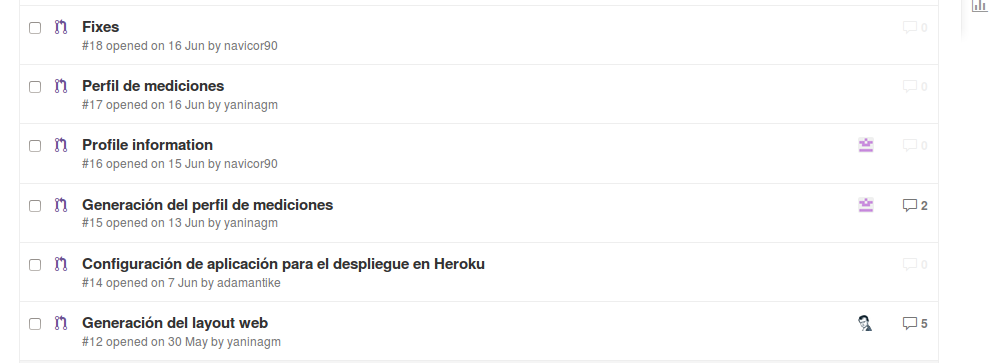
\includegraphics[width=.8\textwidth]{img/2-PR}
  \caption{Pull request realizados por el front end}
  \label{2-PR}
\end{figure}
\begin{figure}[h]
  \centering
  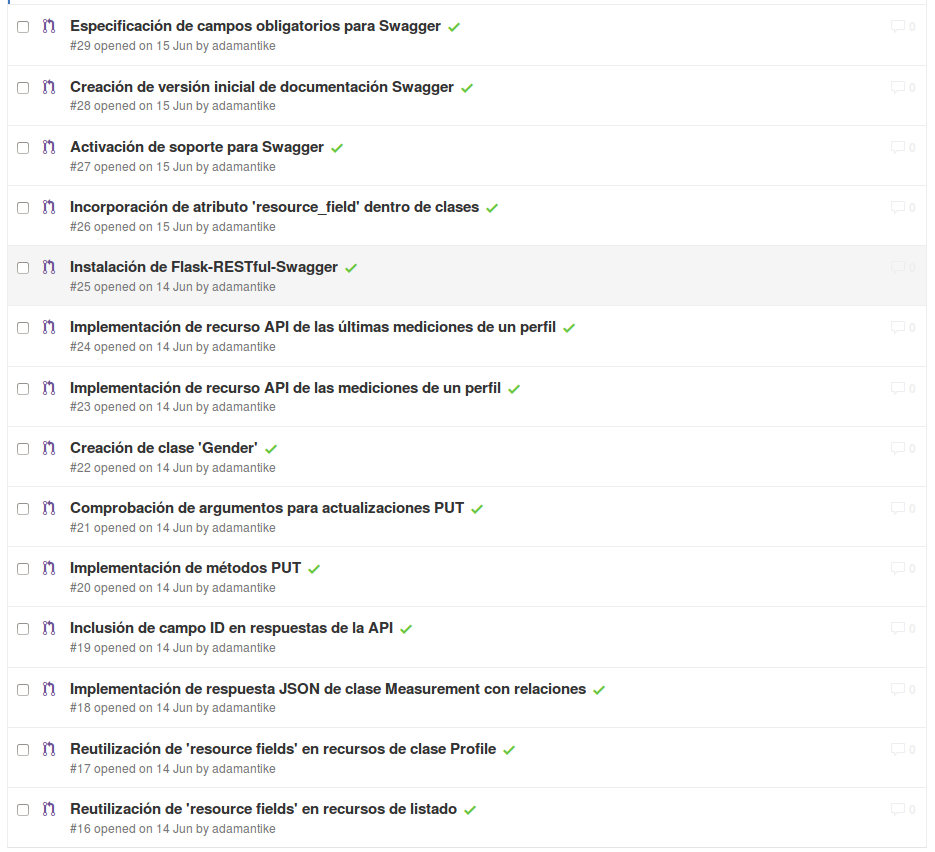
\includegraphics[width=.8\textwidth]{img/2-PR_back2}
  \caption{Pull request realizados por el back end -hoja1}
  \label{2-PR_back2}
\end{figure}
\begin{figure}[h]
  \centering
  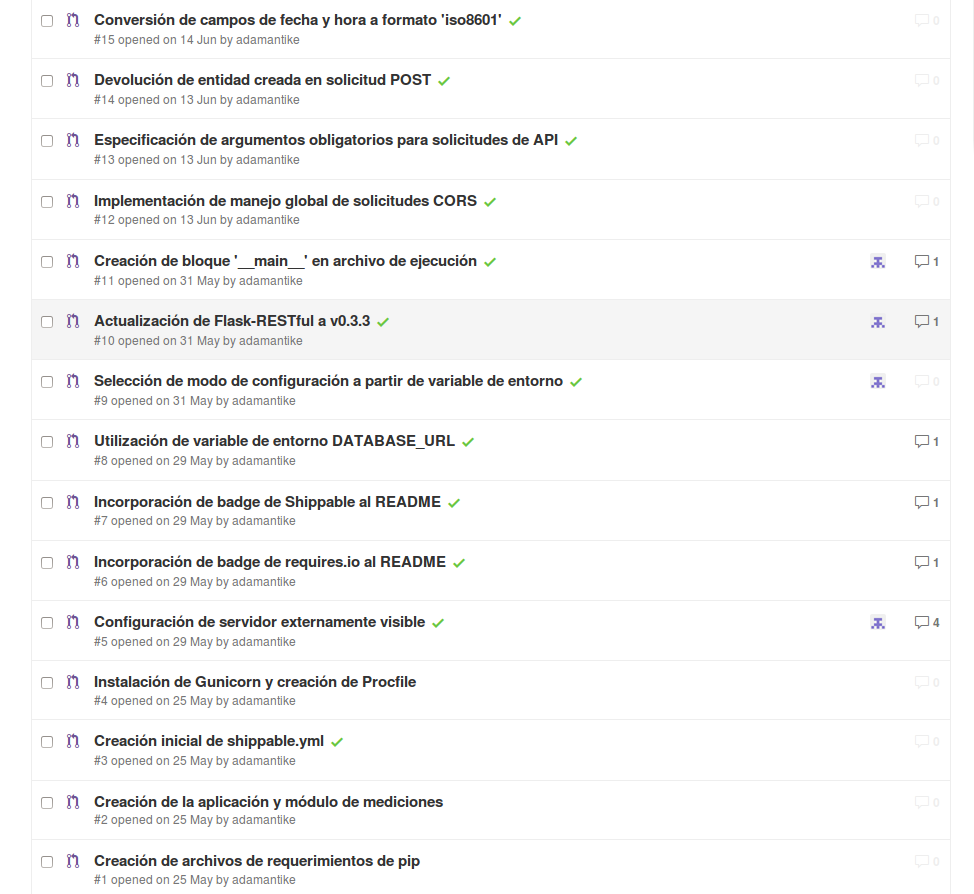
\includegraphics[width=.8\textwidth]{img/2-PR_Back}
  \caption{Pull request realizados por el back end -hoja2}
  \label{2-PR_Back}
\end{figure}

\clearpage
    
	{\scriptsize
		\begin{center} %sidewaystable
			\centering
			%\begin{adjustbox}{max width=\textheight}
			\resizebox{\textwidth}{!}{
				\begin{tabular}{|l|l|l|p{5cm}|l|p{1cm}|}
					\hline
					\textbf{Area a cargo} &
					\textbf{Responsable} &        
					\textbf{Revisor} &        	        
					\textbf{Tarea} &
					\textbf{US} &
					\textbf{Tiempo dedicado} \\
					\hline
					Documentación& Yanina Morales & & Trabajo práctico nº2 y avance de etapa de diseño & US & 20hs\\ \hline        
					Documentación& Ivan Terreno & & Trabajo práctico nº2 y avance de etapa de diseño  &  & 20hs\\ \hline        
					Documentación& Michael Manganiello& & Trabajo práctico nº2 y avance de etapa de diseño  &  & 20hs\\ \hline        
					Documentación& Franco Canizo & & Trabajo práctico nº2 y avance de etapa de diseño  &  & 20hs\\ \hline         
					Front-end& Michael Manganiello& -- & Despliegue de la aplicación en heroku  & US-\ref{resumenInfo} \& US-\ref{infoSalud}& 4 hs  \\ \hline     
					Capacitación & Yanina Morales& & Capacitación en utilización de angular de manera desacoplada& US-\ref{infoSalud}&12 hs\\ \hline        
					Capacitación & Ivan Terreno& & Capacitación en utilización de angular de manera desacoplada& US-\ref{infoSalud}&12 hs\\ \hline                
					Front-end& Ivan Terreno & Michael Manganiello & Generación de controladores para consumir Json de la Api relacionados a la API & US-\ref{resumenInfo} \& US-\ref{infoSalud}& 8hs  \\ \hline
					Front-end & Yanina Morales& Michael Manganiello & Creación de página de formulario de carga de mediciones& US-\ref{infoSalud}&4hs\\ \hline
					Front-end& Ivan Terreno  & Michael Manganiello & Creación de página de formulario de carga de perfil& US-\ref{infoSalud}&4hs\\ \hline
					Front-end& Ivan Terreno  & Michael Manganiello & realización de pruebas& &8hs \\ \hline        
					Front-end&Yanina Morales  & Ivan Terreno  & realización de pruebas & & 12hs\\ \hline         
					
					Back-end& Michael Manganiello & Franco Canizo & Creación de modulo de mediciones&US-\ref{resumenInfo} \& US-\ref{infoSalud} &8hs\\ \hline
					Back-end& Michael Manganiello & ivan Terreno & Exposición de métodos como servicios de API 	& US-\ref{resumenInfo} \& US-\ref{infoSalud}&8hs\\ \hline
					Back-end& Franco Canizo & Michael Manganiello   & Adaptación de salida de métodos a formato Json&US-\ref{resumenInfo} \& US-\ref{infoSalud} &8hs\\ \hline
					Back-end & Franco Canizo & Michael Manganiello  & Carga de valores a la base de datos, relacionados a la API&US-\ref{resumenInfo} \& US-\ref{infoSalud} &8hs \\ \hline
				\end{tabular}
			}
			%\end{adjustbox}
		\end{center}
	}

    
\subsection{Descripción}
En este sprint se llevaran a cabo las interfaces necesarias para que el usuario pueda cargar nuevas mediciones y ver todas sus últimas mediciones ,así teniendo un seguimiento de las mismas con posibilidad de que posteriormente pueda ver su evolución a través de gráficas y tablas.
Para la comunicación de estas interfaces con la API,se desarrollaran los correspondientes adaptadores para los recursos.

Para esto en el backend se deben preparar las clases Measurement, MeasurementType,MeasurementSource,MeasurementUnit con las debidas relaciones con las clase Profile desarrollada en el sprint anterior.
Para cada una de esas clases, se deben preparar interfaces de acceso a los recursos provistos por la API. Y su correspondiente documentación.


\subsection{User Stories relacionados}
La \textbf{Tabla \ref{US-Sprint2}} indicará las características de cada user story para guiarnos en el desarrollo del sprint.

\begin{table}[h]
	%\resizebox{\textwidth}{!}{
    \centering
	\begin{tabular}{|l|p{9cm}|c|}
	\hline
        \multicolumn{1}{|c|}{\textbf{ID}} &
        \multicolumn{1}{|c|}{\textbf{Enunciado de la historia}} &
        \textbf{Prioridad} \\          
    \hline
        US-\ref{resumenInfo} &
        Como paciente quiero obtener un resumen de mi información de salud básica para hacer uso de la misma en caso de una emergencia &Alta
        \\
    \hline 
	    US-\ref{infoSalud} &
        Como paciente quiero cargar mi información personal de salud referido a mediciones (altura, grasa corporal, peso, presión arterial), para que el médico cuente con más y mejor información al momento de realizar el diagnóstico. & Alta
        \\
    \hline
    \end{tabular}
%     }
    \label{US-Sprint2}
\end{table}


\begin{comment}
\subsection{Fase de Análisis}

En esta fase comenzaremos definiendo el Sprint backlog y describiendo en detalle cada una de las tareas que la componen, además se realizará un diagrama de clases iniciales (\textbf{Figura\ref{modelo_datos}}) que nos permitirá guiarnos durante el avance del sprint de ese modo obtener un sistema consistente. 
\end{comment}


\subsection{Modelo de datos}
El Diagrama propio de este sprint se puede ver en la \textbf{Figura\ref{2-modelo_datos_general}}, allí se indican exactamente las clases que se usarán en este sprint y que serán detalladas con detenimiento en el presente documento. Se recuerda que se ha realizado un Diagrama de clases tentativo que se puede ver en la \textbf{Figura \ref{2-modelo_datos_general}}, dicho diagrama  será utilizado como base para este sprint y posee un alcance limitado el cual se irá modificando a medida que se profundice en los temas.



\begin{figure}[h]
  \centering
  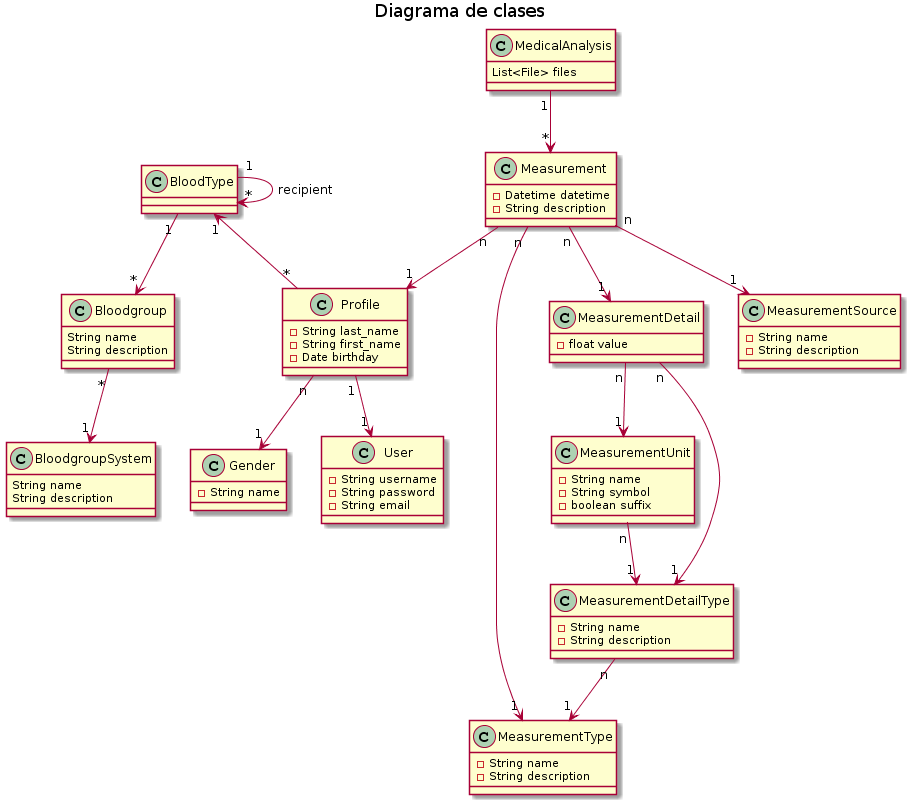
\includegraphics[width=.8\textwidth]{img/2-DC_especifico}
  \caption{Modelo de datos}
  \label{2-modelo_datos_general}
\end{figure}
\clearpage

\subsection{Descripción de las Clases}

\subsubsection{Clase Measurement} 
Dicha clase se refiere a las medición realizada por el usuario en un momento específico. 

\textbf{Descripción de los atributos}
	\begin{itemize}
		\item \textbf{id:} Identificador único de la medición (tipo int).
        \item \textbf{datetime:} Fecha y hora de la medición (tipo datetime).
        \item \textbf{value:} Valor de la medición (tipo float).
        \item \textbf{profile\_id:} Identificador único del perfil asociado (tipo int).
        \item \textbf{measurement\_source\_id:}Identificador único de la fuente de medición asociada (tipo int).
        \item \textbf{measurement\_type\_id:}Identificador único del tipo de medición asociado (tipo int).
        \item \textbf{measurement\_unit\_id:}Identificador único de la unidad de medición asociada (tipo int).
        
	\end{itemize}
    
\textbf{Dirección del recurso:}
\begin{lstlisting}[language=json,firstnumber=1]
<BASE URL>/measurements/{:id}
\end{lstlisting}

\textbf{Json generado por la API}    
\begin{lstlisting}[language=json,firstnumber=1]
{
    "resource": 
{
    "measurement_unit": 
{
    "symbol": "Kg",
    "suffix": true,
    "name": "Kilogramo",
    "id": 1
},
"measurement_source": 
{
    "name": "Manual",
    "description": null,
    "id": 1
},
"value": 50,
"measurement_type": 
{
    "name": "Peso",
    "description": "Peso corporal de la persona.",
    "id": 1
},
"id": 1,
"profile": 
{
    "birthday": "1990-10-26",
    "last_name": "Terreno",
    "first_name": "Milton",
    "gender": 
            {
                "name": "Masculino",
                "description": null,
                "id": 1
            },
            "id": 1
        },
        "datetime": "2015-06-15T02:29:54"
    }
}
\end{lstlisting}
\subsubsection{ Clase MeasurementType }
Esta clase nos permitirá  nomenclar  los tipos de medidas, hasta el momento hemos contemplado: peso, dimensión corporal (Ej:altura) y glucosa. Existen ciertas medidas que contemplan dos valores, estas serán agregadas en un sprint futuro.

\textbf{Descripción de los atributos}
    \begin{itemize}
			\item \textbf{name: }	Nombre del tipo de medición(tipo string).
            \item \textbf{description:} Descripción del tipo de medición (tipo string).
    \end{itemize}

\textbf{Dirección del recurso:}
\begin{lstlisting}[language=json,firstnumber=1]
<BASE URL>/measurement_types/{id}
\end{lstlisting}

\textbf{Json generado por la API} 
\begin{lstlisting}[language=json,firstnumber=1]
{
    "resource": 
    {
        "name": "Peso",
        "description": "Peso corporal de la persona.",
        "id": 1
    }
}
\end{lstlisting}

\subsubsection{ Clase MeasurementUnit }
Esta clase nos permitirá  nomenclar  las unidades de medición disponible para que el usuario pueda seleccionarlas cuando realice la medición, hasta el momento hemos contemplado: Kilogramo, gramo, miligramos, metro, centímetro y milímetro.

    \textbf{Descripción de los atributos}
        \begin{itemize}
            \item \textbf{id:	}	Identificador único de la unidad de medición(tipo int).
            \item \textbf{name :	}	Nombre de la unidad de medición ( tipo string).
            \item \textbf{symbol :}		Símbolo de la unidad de medición (tipo string).
            \item \textbf{suffix :}	Variable booleana que indica si el símbolo de la unidad de medición es un sufijo (verdadero) o un prefijo (falso) del valor de la medición (tipo boolean).
        \end{itemize}

    \textbf{Dirección del recurso}
        \begin{lstlisting}[language=json,firstnumber=1]
        <BASE URL>/measurement_units/{id}
        \end{lstlisting}

    \textbf{Json generado por la API} 
        \begin{lstlisting}[language=json,firstnumber=1]
        {
            "resource": 
            {
                "symbol": "Kg",
                "suffix": true,
                "name": "Kilogramo",
                "id": 1
            }
        }
        \end{lstlisting}

\subsubsection{ Clase MeasurementSource}
Esta clase nos permitirá nomenclar los tipos de fuentes posibles como pueden ser manual, dispositivo móvil, sistema de salud y dispositivo de salud.
    
	\textbf{Descripción de los atributos}
        \begin{itemize}
            \item \textbf{name 	:}	Nombre de la fuente de medición (tipo string).
            \item \textbf{description 	:}	Descripción de la fuente de medición (tipo String).
        \end{itemize}
    \textbf{Dirección del recurso}
    \begin{lstlisting}[language=json,firstnumber=1]
    <BASE URL>/measurement_sources/{:id}
    \end{lstlisting}

    \textbf{Json generado por la API} 
    \begin{lstlisting}[language=json,firstnumber=1]
{
    "resource": 
    {
        "name": "Manual",
        "description": null,
        "id": 1
    }
}
    \end{lstlisting}
    
\subsection{Modelo funcional} %Diagrama de clases
Se describirán las funciones usando como marco de apoyo el sprint Backlog, además se armará el diagrama de casos de uso del presente Sprint \textbf{[Figura \ref{2-caso_de_uso}]} que irá creciendo  medida se vaya avanzando en el proyecto.
    \begin{figure}[h]
        \centering
        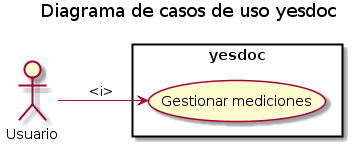
\includegraphics[width=0.5\textwidth]{img/2-caso_de_uso}
        \caption{formulario de edición de perfil}
		\label{2-caso_de_uso}
    \end{figure}

    
\subsubsection{Creación de página de mediciones}
En esta tarea  se generará la pantalla, \textbf{Figura \ref{perfil_medicion}} donde se muestran las mediciones del usuario, como lo son:
      \begin{itemize}
	      \item Altura
          \item Peso
          \item Grasa Corporal
          \item Presión Arterial
      \end{itemize}
      Al igual que en la creación del perfil se dará la posibilidad de acceder a la edición de su perfil desde esta misma página.
      
Para mostrarlas mediciones del usuario es necesario acceder al recurso \texttt{/profiles/\{profile\_id\}/measurements/latest} de la API a través de un método \textbf{GET}


      \textbf{Especificaciones del recursos \texttt{/measurements}}

    \begin{lstlisting}[language=json,firstnumber=1]
          MeasurementFields {
	measurement_source (MeasurementSourceFields, optional),
      profile (ProfileFields),
      datetime (date-time),
      value (number),
      measurement_unit (MeasurementUnitFields),
      id (integer),
      measurement_type (MeasurementTypeFields)
      }
      MeasurementSourceFields {
      description (string, optional),
      id (integer),
      name (string)
      }
      ProfileFields {
      first_name (string),
      last_name (string),
      id (integer),
      gender (GenderFields, optional),
      birthday (date-time, optional)
      }
      GenderFields {
      description (string, optional),
      id (integer),
      name (string)
      }
      MeasurementUnitFields {
      id (integer),
      symbol (string),
      suffix (boolean, optional),
      name (string)
      }
      MeasurementTypeFields {
      description (string, optional),
      id (integer),
      name (string)
      } 
    \end{lstlisting}

    En el perfil de usuario se mostrarán de cada tipo de medición que ha realizado el usuario la última de cada una, indicando el nombre, el valor, el símbolo, la fecha y hora y el método con el que ha sido realizada la medición. Además para cada una de las mediciones se mostrarán dos iconos que corresponden a la edición y a la compartición de las mediciones, este último será implementado en un sprint futuro.

    \begin{figure}[h]
        \centering
        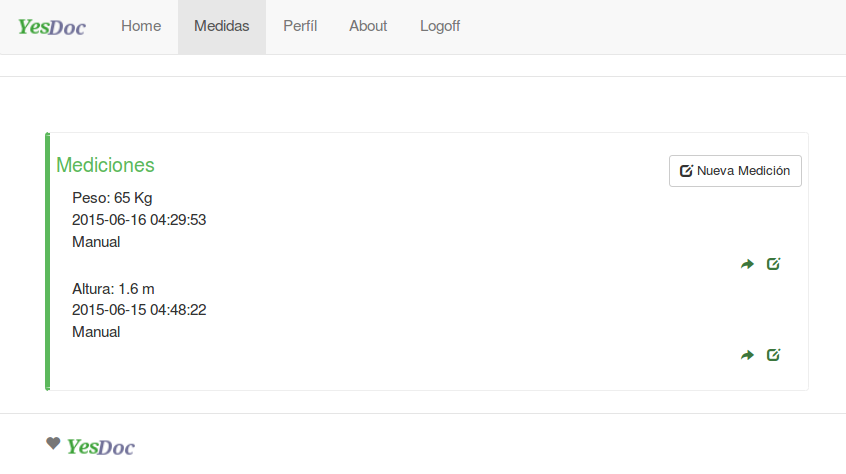
\includegraphics[width=1\textwidth]{img/2-perfil_medicion}
        \caption{Perfil de mediciones}
		\label{perfil_medicion}
    \end{figure}
    
\subsubsection{ Creación de página de formulario de carga de mediciones}
Se generará el formulario necesario, que se muestra en la \textbf{Figura \ref{nueva_medicion}} para que el usuario pueda cargar las mediciones antes nombrados, para ello es necesario acceder al recurso \texttt{/measurements} de la API a través de un método \textbf{POST}

      \begin{lstlisting}[language=json,firstnumber=1]
         MeasurementFields {
        measurement_source (MeasurementSourceFields, optional),
        profile (ProfileFields),
        datetime (date-time),
        value (number),
        measurement_unit (MeasurementUnitFields),
        id (integer),
        measurement_type (MeasurementTypeFields)
        }
        MeasurementSourceFields {
        description (string, optional),
        id (integer),
        name (string)
        }
        ProfileFields {
        first_name (string),
        last_name (string),
        id (integer),
        gender (GenderFields, optional),
        birthday (date-time, optional)
        }
        GenderFields {
        description (string, optional),
        id (integer),
        name (string)
        }
        MeasurementUnitFields {
        id (integer),
        symbol (string),
        suffix (boolean, optional),
        name (string)
        }
        MeasurementTypeFields {
        description (string, optional),
        id (integer),
        name (string)
        } 
    \end{lstlisting}
    
Desde el perfil de mediciones se presentará un icono que representa a la creación de un elemento para que el usuario pueda seleccionarlo. Esta acción llevara al usuario al formulario de creación de mediciones, donde los campos estarán vacíos, para que el usuario los cargue con los valores correspondientes. Una vez terminada la carga, se mostrará un mensaje avisando al usuario que se ha realizado con éxito y luego lo direccionará al perfil de mediciones.
    
    \begin{figure}[h]
        \centering
        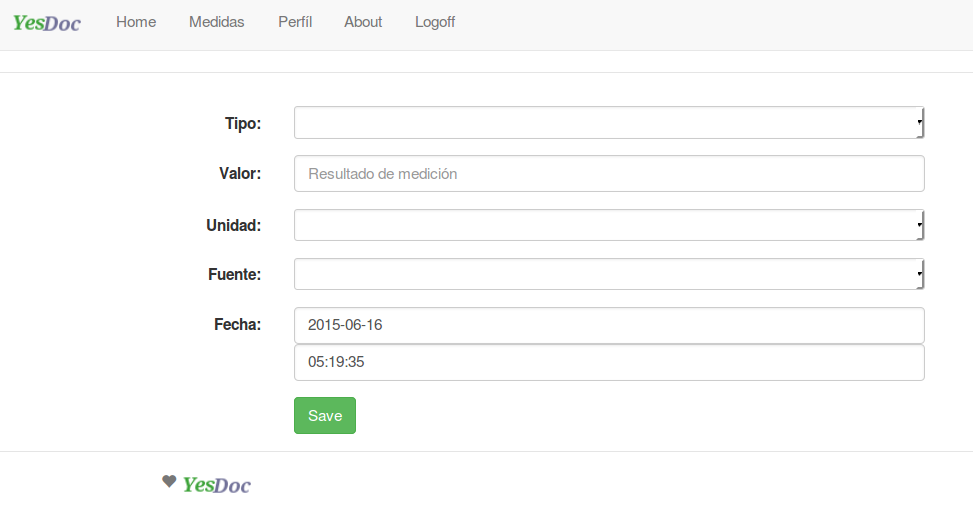
\includegraphics[width=1\textwidth]{img/2-nueva_medicion}
        \caption{Formulario de nueva medición}
		\label{nueva_medicion}
    \end{figure}
\subsubsection{ Creación de página de formulario de edición de mediciones}
Se generará el formulario necesario, que se muestra en la \textbf{Figura \ref{editar_medicion}} para que el usuario pueda editar una medición previamente seleccionada, para ello es necesario acceder al recurso \texttt{/measurements/\{:id\}} a través del método \textbf{PUT} enviando por URL el id correspondiente a dicha medición. 

Desde el perfil de mediciones se presentará un icono que representa a la edición de un elemento para que el usuario pueda seleccionarlo. Esta acción llevara al usuario al formulario de edición de mediciones, donde los campos estarán cargados con los valores antiguos, de este modo el usuario modifica lo que desea y no tiene que cargar todo nuevamente. Una vez terminada la edición se direccionará al perfil de mediciones.

	\begin{figure}[h]
        \centering
        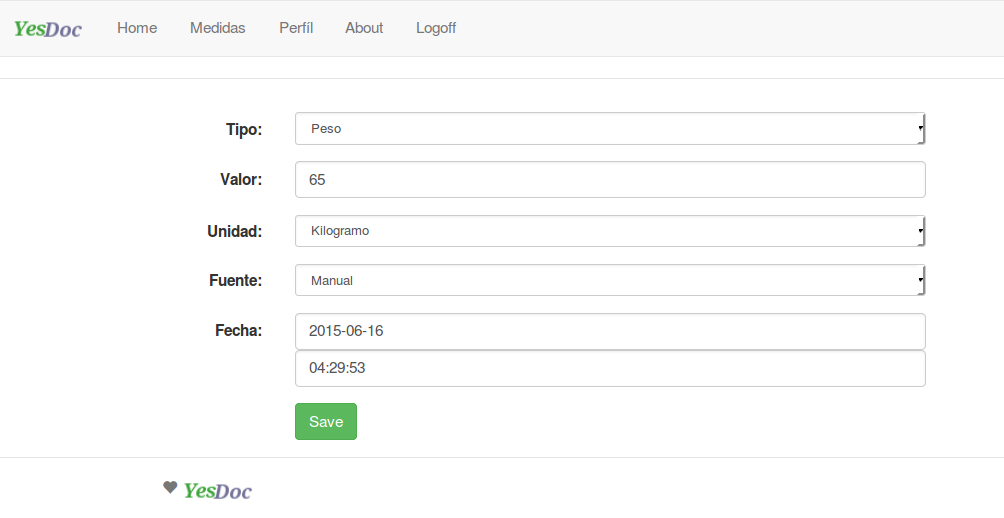
\includegraphics[width=1\textwidth]{img/2-editar_medicion}
        \caption{Formulario de edición de medición}
		\label{editar_medicion}
    \end{figure}
    
%%%%%%%%%%%%%%%%%%%%%% COMPLETAR!!! %%%%%%%%%%%%%%%%%%%%%%%%%%%%
\begin{comment}


\subsubsection{Creación de aplicación  }
\subsubsection{Creación de modulo de mediciones}
\subsubsection{Exposición de métodos como servicios de API}
\subsubsection{ Adaptación de salida de métodos a formato Json}
\subsubsection{Creación de base de datos inicial}
\end{comment}

\subsection {Salidas del Sistema - Incrementos}

Luego de finalizado este user story se obtendrán 4 pantallas que se detallarán a continuación:
\begin{enumerate}
    \item \textbf{Presentación de las últimas mediciones}  \textbf{[Figura  \ref{perfil_medicion}]} con posibilidad de edición de cada una de las mediciones. Los datos posible  a presentar son altura, peso, grasa corporal y glucosa. 
    
    La interfaz mostrará el valor de la medición, la fecha y hora en que fue realizada y la fuente que se utilizó para dicha medición.
	\item \textbf{Carga de mediciones}: \textbf{[Figura \ref{nueva_medicion}]} Se le permitirá cargar mediciones que realice en algún momento del día como son peso, altura, grasa corporal y glucosa. Deberá indicar la fuente, tipo, unidad y fecha de la medición
    \item \textbf{Edición de mediciones:}  \textbf{[Figura \ref{editar_medicion}]} Se le permitirá seleccionar una medición del perfil de mediciones para sel modificada.

\end{enumerate}

    




\subsection{Criterios de aceptación}

\begin{center}
\begin{longtable}{|p{0.5cm}|p{4cm}|p{4cm}|p{5cm}|}
\hline \hline \rowcolor[gray]{0.9}
	\multicolumn{4}{||c|}{\textbf{Criterio de aceptación}} \\
    \hline  \rowcolor[gray]{0.9}
        \textbf{Id} &
        \textbf{Contexto} &
        \textbf{Evento}&
        \textbf{Resultado} \\
    \hline
1&En caso de que exista una persona sin mediciones & cuando este desee observar sus mediciones  & El sistema no mostrará nada \\ \hline
 
2& Cuando el usuario registrado ingresa dos mediciones del mismo tipo  & y luego quiera consultarlas & El sistema solo le mostrará la ultima medición, del mismo tipo, realizada\\ \hline

3& Cuando el usuario seleccione una medición & y luego quiera editarla & El sistema le permitira la correspondiente edición\\ \hline

4& Si el usuario existe y no está logeado & y quiera ingresar a ver sus mediciones. & El sistema no le permitirá ingresar\\ \hline
  \end{longtable}
\end{center}


\subsection{Casos de Prueba}


	{\scriptsize
	\begin{table}[h]
	\centering
	\begin{tabular}{||l|p{10cm}||}
    	\rowcolor[gray]{0.9}
	    \hline 
        \hline 
	    \textbf{Caso de prueba} & \textbf{Consultar mediciones (sin medidas precargadas)}\\  \hline
	    \textbf{Descripción del escenario}& Nombre: Marita; Apellido Martinez; fecha de Nacimiento:20-08-1989; id:3  \\ \hline
	    \textbf{Criterio de aceptación}&  \textbf{En caso de que exista una persona sin mediciones cargadas, si el usuario desea verlas el sistema no debería mostrar ninguna medición } \\ \hline
        \textbf{Datos de entrada}&  consultar mediciones\\ \hline
        \textbf{Condiciones de  prueba}& Se necesita que esté previamente cargado el usuario "Marita Martinez" y no tenga datos más allá de su nombre y apellido en el perfil \\ \hline \hline
	    \end{tabular}
        \caption{Caso de prueba para criterio de aceptación 1}
    	\end{table}
	}
  
{\scriptsize
	\begin{table}[h]
    \centering
	\begin{longtable}{|p{5cm}|p{5cm}|p{5cm}|}
	    \hline \hline \rowcolor[gray]{0.9}
        \multicolumn{3}{||l|}{\textbf{Procedimiento de Prueba - ``Consultar mediciones''}} \\
        \hline \rowcolor[gray]{0.9}
		    \textbf{Actor} & 
	        \textbf{Sistema}& 
        	\textbf{Resultado Esperado} \\  
        \hline
	    El usuario ingresa al sistema con su id nº3	& &\\ \hline
        		& El sistema valida con los perfiles de la API si el Id:3 del usuario existe& Se presenta por pantalla el perfil del usuario con sus datos  \\ \hline        
	    El usuario selecciona la pestaña mediciones y realiza la consulta& &\\ \hline
      	&El sistema valida que las cookies estén activas&\\ \hline
   		&El sistema solicita a la API las mediciones del perfil con id:3&El sistema no muestra ninguna medida cargada \\ \hline 
	    \end{longtable}
		\caption{Procedimiento de prueba para criterio de aceptación 1}
    	\end{table}
	}
    
        {\scriptsize
	\begin{table}[h]
	\centering
	\begin{tabular}{|l|p{10cm}|}
	    \hline 
	    \textbf{Salida obtenida}& No se presentan datos de mediciones\\ \hline
	    \textbf{Resultado}& \textbf{Correcto}\\ \hline
        \textbf{¿Que fue mal?}& Nada\\ \hline      
        \textbf{Evidencia}& \\ \hline
        \textbf{Seguimiento}&No es necesario ya que el caso de prueba no causó
fallos \\ \hline
        \textbf{Estado}& \textbf{Terminado}\\ \hline        
         \textbf{¿Que se puede mejorar?}& En otra iteración se debería añadir carteles de avisos, informando que faltan cargar datos \\ \hline              
	    \end{tabular}
        \caption{Resultado esperado para el criterio de aceptación 1}
    	\end{table}
	}
\clearpage 
%%%%%%%%%%%%%%%%%%%%%%%%%%%%%%%%%%%%%%%%%%%%%%%%%%

{\scriptsize
	\begin{table}[h]
	\centering
	\begin{tabular}{||l|p{9cm}||}
    	\rowcolor[gray]{0.9}
	    \hline 
        \hline 
	    \textbf{Caso de prueba}  &  \textbf{Consultar mediciones (medida precargada)}\\  \hline
	    \textbf{Descripción del escenario}& Nombre: Marita; Apellido Martinez; fecha de Nacimiento:20-08-1989; id:3; altura: 2m  \\ 			\hline
	    \textbf{Criterio de aceptación} &\textbf{ Cuando el usuario registrado ingresa dos mediciones del mismo tipo y luego quiera consultarlas. El sistema solo le mostrará la ultima medición, del mismo tipo, realizada} \\ \hline
        \textbf{Datos de entrada}& id:3; Peso 1: 67kg; peso 2: 55kg \\ \hline
        \textbf{Condiciones de  prueba}& el usuario Marita Martinez existe \\ \hline 			\hline
	    \end{tabular}
        \caption{Caso de prueba para criterio de aceptación 2}        
	    \end{table}
}
 
   %{\scriptsize
	\begin{longtable}{|p{5cm}|p{5cm}|p{4cm}|}
 
	    \hline \hline \rowcolor[gray]{0.9}
        \multicolumn{3}{||l|}{\textbf{Procedimiento de Prueba - Consultar mediciones}} \\ \hline
	    \hline 
        \rowcolor[gray]{0.9}
	    \textbf{Actor} & \textbf{Sistema}& \textbf{Resultado Esperado} \\  \hline
	    El usuario se logea en el sistema& & \\ \hline
        & El sistema consulta la API para corroborar que el perfil con id:3 existe &\\ \hline
        &  El sistema redirecciona al usuario a la vista de perfil de usuario&Se muestra el perfil de usuario con los datos respectivos\\ \hline
	    El usuario selecciona la pestaña de mediciones de la barra de navegación& &\\ \hline
        & El sistema verifica las cookies del usuario para determinar si ya se encuentra logeado &\\ \hline
        & El sistema redirecciona al usuario a la vista de mediciones&Se muestra la vista de mediciones con las últimas mediciones del usuario correspondientes\\ \hline  
        El usuario selecciona el botón de añadir ``nueva medicion''& &\\ \hline       
        & El sistema verifica que las cookies posean los datos del usuario&\\ \hline       
        & Se redirecciona a la vista de carga de mediciones&Se presenta el formulario de medición para la carga respectiva\\ \hline
        El usuario selecciona: Tipo de medicion: Peso; medida 55; unidad: Kg; Fuente: manual; fecha: deja la precargada y  luego de esto presiona el botón save& &\\ \hline       
        & El sistema valida que estén todos los datos cargado, excepto fuente el cual no es necesario, carga los nuevos datos en la API a través del método POST y redirecciona a la vista de mediciones&\\ \hline       
        &El sistema a través del método GET trae las últimas mediciones. &Se muestran las últimas mediciones en la vista de mediciones\\ \hline
        El usuario presiona el botón ´´cargar mediciones'' nuevamente& &\\ \hline  
        & El sistema verifica que las cookies posean los datos del usuario&\\ \hline       
        & Se redirecciona a la vista de carga de mediciones&Se presenta el formulario de mediciones para la carga respectiva\\ \hline
        El usuario selecciona: Tipo de medicion: Peso; medida 67; unidad: Kg; Fuente: manual; fecha: deja la precargada y  luego de esto presiona el botón save& &\\ \hline       
        & El sistema valida que estén todos los datos cargado, excepto fuente el cual no es necesario, carga los nuevos datos en la API a través del método POST y redirecciona a la vista de mediciones&\\ \hline       
        &El sistema a través del método GET trae las últimas mediciones. &El sistema muestra la última medición cargada ``Peso 55 Kg, fecha de carga y método: manual\\ \hline
        \caption{Procedimiento de prueba para criterio de aceptación 2}
        
	    \end{longtable}
        
	%}
\clearpage

{\scriptsize
	\begin{table}[h]
	\centering
	\begin{tabular}{|l|p{10cm}|}
	    \hline 
	    \textbf{Salida obtenida}& Se mostraron correctamente la ultima medición del mismo tipo\\ \hline
	    \textbf{Resultado}& \textbf{Correcto}\\ \hline
        \textbf{¿Que fue mal?}& Nada\\ \hline      
        \textbf{Evidencia}& En Listing \ref{JsonMediciones} se puede observar que el usuario posee 3 mediciones, dos de las cuales son del mismo tipo (tipo Peso) y en la Figura \ref{perfil_id_3} se puede ver que solo se muestra la última medición del Peso.  \\ \hline
        \textbf{Seguimiento}& no es necesario\\ \hline
        \textbf{Estado}& \textbf{Terminado}\\ \hline        
        \textbf{¿Que se puede mejorar?}& \\ \hline              
	    \end{tabular}
        \caption{Resultado esperado para el criterio de aceptación 2}
    	\end{table}
	}


{\scriptsize
%\begin{minipage}{1 \textwidth}
    \begin{lstlisting}[language=json,firstnumber=1,  breaklines=true, caption= Json de las mediciones del perfil id:3, label=JsonMediciones]

        {"resource": 
	        [{
	    	    "measurement_source": 
        		{
		            "id": 1,
        		    "description": null,
		            "name": "Manual"
        		},
		        "measurement_type": 
        		{
		            "id": 1,
		            "description": "Peso corporal de la persona.",
		            "name": "Peso"
		        },
        		"datetime": "2015-07-03T11:51:39.436000",
		        "value": 55,
		        "id": 16,
    	    	"measurement_unit": 
                {
             	   "id": 1,
	               "suffix": true,
	               "name": "Kilogramo",
	               "symbol": "Kg"
	             }
    	    },
        	{
            	"measurement_source": 
		        {
        		    "id": 1,
		            "description": null,
		            "name": "Manual"
		        },
	        	"measurement_type": 
    		    {
	        	    "id": 1,
		            "description": "Peso corporal de la persona.",
		            "name": "Peso"
		        },
        		"datetime": "2015-07-03T11:54:22.806000",
		        "value": 67,
		        "id": 17,
        	"measurement_unit": 
	            {
    	            "id": 1,
        	        "suffix": true,
            	    "name": "Kilogramo",
                	"symbol": "Kg"
                }
              },
              {"measurement_source": 
                {
                    "id": 0,
                    "description": null,
                    "name": null
                },
               "measurement_type": 
                {
                    "id": 2,
                    "description": "Longitud de la persona",
                    "name": "Altura"
                },
	                "datetime": "2015-07-03T13:05:57.375000",
    	            "value": 2,
        	        "id": 18,
                "measurement_unit": 
                    {
                        "id": 2,
                        "suffix": true,
                        "name": "Metros",
                        "symbol": "m"
                    }
    	    }]
        }   
    \end{lstlisting}   


\begin{figure}[h]
        \centering
        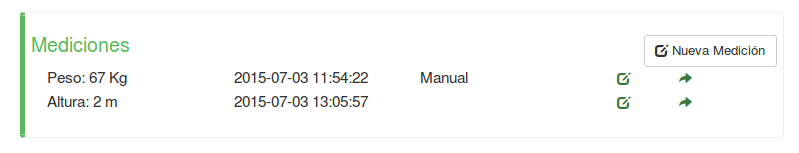
\includegraphics[width=1\textwidth]{img/2-prueba_2}
        \caption{perfil de medicion de usuario con id:3}
		\label{perfil_id_3}
\end{figure}


%\end{minipage}
    }
\clearpage

%%%%%%%%%%%%%%%%%%%%%%%%%%%%%%%%%%%%%%%%%%%%%%%%%%%%%%%%%

{\scriptsize
	\begin{table}[h]
	\centering
	\begin{tabular}{||l|p{10cm}||}
    	\rowcolor[gray]{0.9}
	    \hline 
        \hline 
	    \textbf{Caso de prueba} & \textbf{Editar Medición}\\  \hline
	    \textbf{Descripción del escenario}&  Nombre: Marita; Apellido Martinez; fecha de Nacimiento:20-08-1989; id:3; id:3; Peso 1: 67kg, id:17; peso 2: 55kg, id:16\\ \hline
	    \textbf{Criterio de aceptación}& \textbf{Cuando el usuario seleccione una medición  y luego quiera editarla. El sistema le permitirá la correspondiente edición}\\ \hline
        \textbf{Datos de entrada}& peso:65Kg \\ \hline
        \textbf{Condiciones de  prueba}& Usuario logueado con al menos una medida cargada \\ \hline \hline
	    \end{tabular}
	    \end{table}
	}
    

	\begin{longtable}{|p{5cm}|p{5cm}|p{4cm}|}
	    \hline \hline \rowcolor[gray]{0.9}
        \multicolumn{3}{||l|}{\textbf{Procedimiento de Prueba - Editar mediciones}} \\ \hline
	    \hline 
        \rowcolor[gray]{0.9}
	    \textbf{Actor} & \textbf{Sistema}& \textbf{Resultado Esperado} \\  \hline
	    El usuario, ya logueado selecciona el botón de editar de una de las mediciones (medición peso 67Kg) que se muestra en su perfil de mediciones& & \\ \hline
        & El sistema valida las que las cookies estén activas & \\ \hline
        & El sistema consulta a la API la medición 17 correspondiente al perfil con id:3 & Se muestra el perfil del formulario de carga de mediciones. con los datos precargados de la medición seleccionada\\ \hline        
	    El usuario modifica los datos de la medición seleccionada cambiando 67 por 65&  &\\ \hline
        & el sistema confirma la carga guardando los datos en la API a través del método PUT&\\ \hline
        &El sistema redirecciona al usuario a la vista de perfil de mediciones&  Se le presenta al usuario la vista de las ultimas mediciones realizadas. Mostrando 65Kg \\ \hline
        		\caption{Procedimiento de prueba para criterio de aceptación 3}
	    \end{longtable}
	
            {\scriptsize
	\begin{table}[h]
	\centering
	\begin{tabular}{|l|p{10cm}|}
	    \hline 
	    \textbf{Salida obtenida}& La vista presento la medición modificada de forma correcta\\ \hline
	    \textbf{Resultado}& \textbf{Correcto}\\ \hline
        \textbf{¿Que fue mal?}& Nada\\ \hline      
        \textbf{Evidencia}&  En la figura \ref{edicion_medicion} se puede ver como el formulario se encuentra precargado con los valores de la medición que se desea editar, en el Json \ref{JsonMedicionModificada} se puede observar que se modifico el valor del peso y que ha cambiado la fecha de carga \\ \hline
        \textbf{Seguimiento}& No es necesario ya que el caso de prueba no causó
fallos\\ \hline
        \textbf{Estado}& \textbf{Terminado}\\ \hline        
        \textbf{¿Que se puede mejorar?}& En otro sprint se debería añadir carteles de avisos, informando que la edición fue realizada con éxito \\ \hline              
	    \end{tabular}
        \caption{Resultado esperado para el criterio de aceptación 3}
    	\end{table}
	}
\begin{figure}[h]
        \centering
        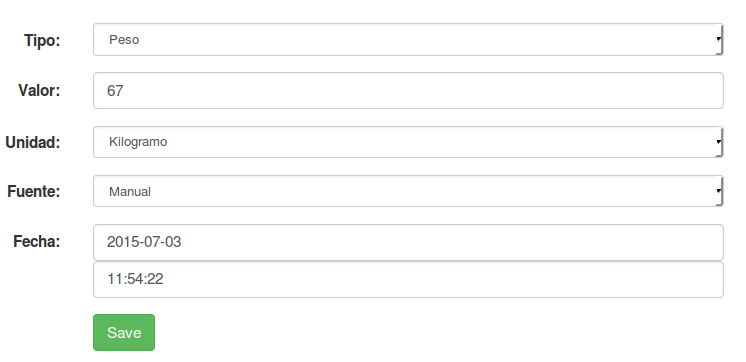
\includegraphics[width=1\textwidth]{img/2-prueba_3}
        \caption{Formulario de edición de medición}
		\label{edicion_medicion}
\end{figure}

\begin{lstlisting}[language=json,firstnumber=1,  breaklines=true, caption= Json de las medicion modificada del perfil id:3, label=JsonMedicionModificada]
{
	"id": 17,
    "measurement_source": 
	{
    	"id": 1,
	    "description": null,
	    "name": "Manual"
	},
	"measurement_unit": 
	{
    "id": 1,
    "suffix": true,
    "symbol": "Kg",
    "name": "Kilogramo"
	},
	"measurement_type": 
    {
        "id": 1,
        "description": "Peso corporal de la persona.",
        "name": "Peso"
    },
    "value": 65,
    "datetime": "2015-07-03T11:54:22.806000"
}
\end{lstlisting}
\clearpage  

%%%%%%%%%%%%%%%%%%%%%%%%%%%%%%%%%%%%%%%%%%%%%%%%%%%%%%%%%
		{\scriptsize
    \begin{table} [h]
    \centering
	\begin{tabular}{||l|p{10cm}||}
    	\rowcolor[gray]{0.9}
	    \hline 
        \hline 
		\textbf{Caso de prueba} & \textbf{Ingresar a mediciones} \\  \hline
	    \textbf{Descripción del escenario}& Nombre: Marita; Apellido Martinez; fecha de Nacimiento:2015-06-01; género: femenino; id:3; Peso 1: 54kg; peso 2: 55kg\\ \hline
	    \textbf{Criterio de aceptación}&\textbf{Si el usuario existe y no está logueado y quiere ingresar a ver sus mediciones. El sistema no le permitirá ingresar}\\ \hline
        \textbf{Datos de entrada}&  \\ \hline
        \textbf{Condiciones de  prueba}& El usuario no debe encontrase logueado.\\ \hline \hline
	    \end{tabular}
        \caption{Caso de prueba para criterio de aceptación 4}
    	\end{table}
		}
	

	\begin{longtable}{|p{5cm}|p{5cm}|p{5cm}|}
	    \hline \rowcolor[gray]{0.9}
        \multicolumn{3}{|l|}{\textbf{Procedimiento de Prueba -Ingresar mediciones}} \\ \hline
	    \textbf{Actor} & \textbf{Sistema}&\textbf{Resultado Esperado} \\  \hline
	   El usuario selecciona la pestaña de mediciones, para ver sus mediciones & & \\ \hline
        & El sistema  verifica que exista una cookies activa como na existe no lo redirección a ninguna parte &  Se muestra la ventana de logueo \\ \hline
   \caption{Procedimiento de prueba para criterio de aceptación 4}        
    \end{longtable}
 


{\scriptsize
	\begin{table}[h]

	\centering
	\begin{tabular}{|l|p{10cm}|}
	    \hline 
	    \textbf{Salida obtenida}&Se obtuvo lo q se esperaba, ya que no fue enviado a la vista de mediciones.\\ \hline
	    \textbf{Resultado}& \textbf{Correcto}\\ \hline
        \textbf{¿Que fue mal?}& Nada\\ \hline        
        \textbf{Evidencia}&No es necesaria  \\ \hline
        \textbf{¿Que fue mal?}& Nada\\ \hline      
        \textbf{Seguimiento}& No es necesario ya que el caso de prueba no causó fallos \\ \hline
        \textbf{Estado}& \textbf{Terminado}\\ \hline        
        \textbf{¿Que se puede mejorar?}& En una futura iteración se podría añadir carteles de avisos informando de la situación\\ \hline              
	    \end{tabular}
        \caption{Resultado esperado para el criterio de aceptación 4}
   	\end{table}
	}

%%%%%%%%%%%%%%%%%%%%%%%%%%%%%%%%%%%%%%%%%%%%%%%%%%%%%%%%%%%%%%%%%%

\clearpage
\subsubsection{Pruebas  de  integración  entre módulos del Sistema}
Estas pruebas se realizarán mas adelantes
\subsubsection{ Pruebas de carga}
En este sprint no se realizarán este tipo de pruebas.
\subsubsection{ Pruebas de seguridad por niveles de usuarios}
En este sprint no se realizarán este tipo de pruebas, ya que la seguridad será un tema a tratar más adelante.

\subsection{Pruebas ejecutadas}
Aqui se realizará una conclusión general de lo que se descubrió en las pruebas.
        %
	\begin{itemize}
		\item \textbf{¿Que fue bien?}
        	\begin{itemize}
				\item        Las cargas y ediciones se llevan a cabo correctamente.
			\end{itemize}

   		\item \textbf{¿Que se mejoró?}
        	\begin{itemize}
				\item \textbf{Cerrado} Al crear una nueva medición, se mostraba un cartel (alert de javascript) con una fecha, dicho alert fue eliminado.
                \item \textbf{Cerrado} Se encontró un problema con la zona horaria que usa el servidor y la zona horaria del usuario, para solucionarlo hubo q hacer un casteo previo cuando se solicitaba la fecha y hora del usuario para mostrar.
			\end{itemize}

   		\item \textbf{¿Que se puede mejorar?}
        	\begin{itemize}
		        \item \textbf{Abierto} En el futuro se deberá mejorar las validaciones de los datos a la hora de cargar información en los formularios.
        		\item \textbf{Abierto} Se deberá mejorar la manera de seleccionar la fecha y la hora.
		        \item \textbf{Abierto} Solo debería mostrarse las unidades relacionadas al tipo de medición que se ha seleccionado  
                \item \textbf{Abierto} Deberá realizarse los carteles de advertencia necesarios.
            \end{itemize}
        

	\end{itemize}


%%%%%%%%%%%%%%%%%%%%%%%%%%      FIN SPRINT 2  %%%%%%%%%%%%%%%%%%%%%%%%%

\section{Sprint 3}%Corrección de issues 
\subsection{Planificación}

\textbf{Inicio: }Martes 7 de julio del 2015 

\textbf{Fin:} Martes 16 de Agosto del 2015

\begin{figure}[h!]
  \centering
  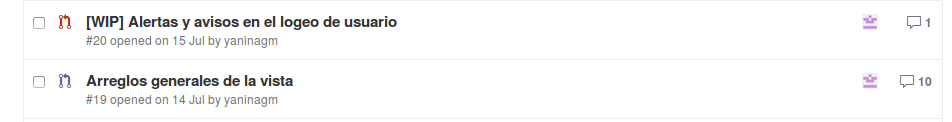
\includegraphics[width=.8\textwidth]{img/3-PR_1_front}
  \caption{Pull request realizados en el sprint  3}
  \label{pull_request_sprint_3}
\end{figure}
\begin{figure}[h!]
  \centering
  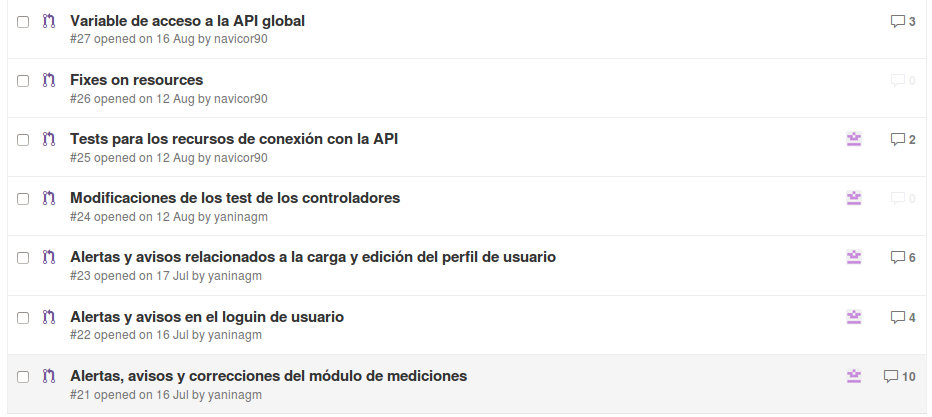
\includegraphics[width=.8\textwidth]{img/3-PR_2_front}
  \caption{Pull request realizados en el sprint  3}
  \label{3-PR_back}
\end{figure}

	{\scriptsize
	\begin{center} %sidewaystable
	\centering
	%\begin{adjustbox}{max width=\textheight}
    \resizebox{\textwidth}{!}
    {
	\begin{tabular}{|l|l|p{5cm}|l|l|}
	    \hline
	        \textbf{Area a cargo} &
	        \textbf{Responsable} &        
	        \textbf{Tarea} &
	        \textbf{US} &
            \textbf{Tiempo}\\
   		\hline
       
	    Documentación& Michael Manganiello & trabajo práctico integrador nº2 ``Planificación de proyectos informáticos''. & & 17hs \\ \hline
        Documentación& Ivan Terreno & trabajo práctico integrador nº2 ``Planificación de proyectos informáticos''. & & 17hs \\ \hline
        Documentación& Morales Yanina & trabajo práctico integrador nº2 ``Planificación de proyectos informáticos''. & & 17hs \\ \hline
        Documentación& Franco Canizo & trabajo práctico integrador nº2 ``Planificación de proyectos informáticos''. & & 17hs \\ \hline
        Presentaciones& Todos & Postulación del proyecto la BAIT 2015. & & 4hs \\ \hline
        Presentaciones& Todos & Preparación de la presentación en BAIT 2015. & & 15hs \\ \hline        
	    Front-end& Yanina Morales & Creación de validadores y mensajes de alerta & & 10hs\\ \hline   
	    Front-end& Yanina Morales & Generación de pruebas automatizadas para la carga y muestra de datos personales& & 10hs\\ \hline  
	    Front-end& Ivan Terreno & Generación de pruebas automatizadas para la carga y muestra de mediciones & & 10hs\\ \hline  	              
	    \end{tabular}
        }
	    %\end{adjustbox}
    	\end{center}
	}


\subsection{Descripción}
%navbar responsive
En este sprint se corregirán los errores detectados en las pruebas realizadas con anterioridad en los sprint referidos a:
    \begin{itemize}
    \item Generar perfil de datos personales.
    \item Generar  perfil de mediciones.
    \end{itemize}
Cabe destacar que sólo se documentarán aquellas correcciones que se refieran a las funcionalidades a documentar ``Carga y muestra de mediciones''

Se desarrollarán las interfaces que permiten mostrar las gráficas de las mediciones de un usuario.

Y se realizarán las validaciones necesarias para que el sistema funcione correctamente.


Además en este Sprint el equipo se presentó y quedó como finalista en el  concurso ``Premio a la Innovación Tecnológica'', organizado por el Polo IT de Buenos Aires, teniendo que organizar la presentación a mostrar. Para ellos se realizó un vídeo de presentación, una página web, tarjetas de contacto y se preparo un speech elevator para conquistar al público


\subsection{User Stories relacionados}
La \textbf{Tabla \ref{US-Sprint3} } indicará las características de cada user story para guiarnos en el desarrollo del sprint.

\begin{table}[h]
    \label{US-Sprint3}
	%\resizebox{\textwidth}{!}{
    \centering
	\begin{tabular}{|l|p{9cm}|}
	\hline
        \multicolumn{1}{|c|}{\textbf{ID}} &
        \multicolumn{1}{|c|}{\textbf{Enunciado de la historia}} \\          
    \hline
        \textbf{US-2 } & Como paciente, quiero añadir al sistema los estudios realizados para evitar posibles perdidas.\\
     \hline 
        \textbf{US-5 } & Como paciente quiero que los sistemas de salud existentes puedan cargar sus resultados directamente en mi carpeta de salud para centralizar mi información. \\
      \hline 
        \textbf{US-7} & Como paciente quiero categorizar mis estudios por rama de medicina, para lograr una mejor organización y navegabilidad en el sistema. \\
       \hline 
        \textbf{US-8} & Como laboratorio, quiero cargar información de un paciente en su cuenta para ahorrarle las molestias de volver. \\
        \\
    \hline 
	    \textbf{US-17} &   Como paciente quiero ver gráficas que resuman mi información en particular para poder ver mis cambios a lo largo de la historia.\\
    \hline        
        \textbf{US-15} & Como médico quiero ver gráficas que resuman la información de un paciente para poder ver sus cambios a lo largo de la historia y así apoyar la toma de decisiones y el diagnóstico.\\
    \hline
    \end{tabular}
%     }

\end{table}

\subsection{Clases involucradas}
\label{3-clases_involucradas}
\begin{figure}[h!]
	\centering
	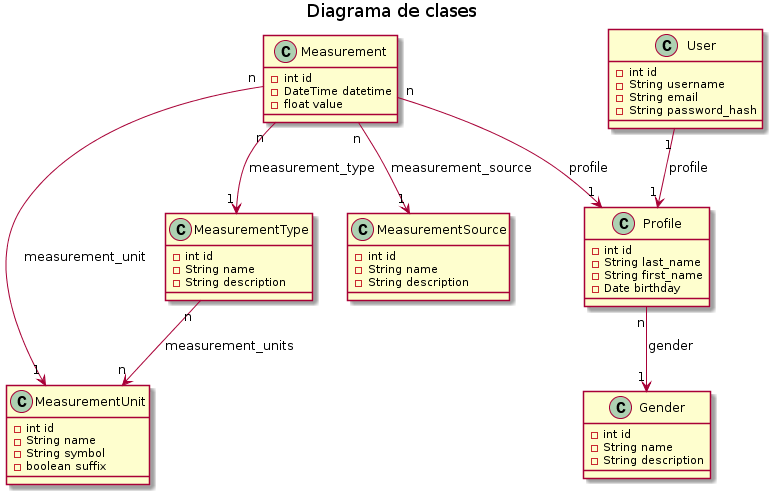
\includegraphics[width=.8\textwidth]{img/3-diagramaClases_relacionTipos}
	\caption{Diagrama de clases donde se puede ver la relación entre el tipo de medición y la unidad}
	\label{relacion_tipo}
\end{figure}


\textbf{ Clase MeasurementType }

Esta clase nos permitirá  nomenclar  los tipos de medidas, hasta el momento hemos contemplado: peso, dimensión corporal (Ej:altura) y glucosa. Existen ciertas medidas que contemplan dos valores, estas serán agregadas en un sprint futuro.

\textbf{Descripción de los atributos}
\begin{itemize}
	\item \textbf{name: }	Nombre del tipo de medición(tipo string).
	\item \textbf{description:} Descripción del tipo de medición (tipo string).
\end{itemize}

\textbf{Dirección del recurso:}
\begin{lstlisting}[language=json,firstnumber=1]
<BASE URL>/measurement_types/{id}
\end{lstlisting}

\textbf{Json generado por la API} 
\begin{lstlisting}[language=json,firstnumber=1]
{
"resource": 
{
"name": "Peso",
"description": "Peso corporal de la persona.",
"id": 1
}
}
\end{lstlisting}

\textbf{ Clase MeasurementUnit }

Esta clase nos permitirá  nomenclar  las unidades de medición disponible para que el usuario pueda seleccionarlas cdo realice la medición, hasta el momento hemos contemplado: Kilogramo, gramo, miligramos, metro, centímetro y milímetro.

\textbf{Descripción de los atributos}
\begin{itemize}
	\item \textbf{id:	}	Identificador único de la unidad de medición(tipo int).
	\item \textbf{name :	}	Nombre de la unidad de medición ( tipo string).
	\item \textbf{symbol :}		Símbolo de la unidad de medición (tipo string).
	\item \textbf{suffix :}	Variable booleana que indica si el símbolo de la unidad de medición es un sufijo (verdadero) o un prefijo (falso) del valor de la medición (tipo boolean).
\end{itemize}

\textbf{Dirección del recurso}
\begin{lstlisting}[language=json,firstnumber=1]
<BASE URL>/measurement_units/{id}
\end{lstlisting}

\textbf{Json generado por la API} 

\begin{lstlisting}[language=json,firstnumber=1]
{
"resource": 
{
"symbol": "Kg",
"suffix": true,
"name": "Kilogramo",
"id": 1
}
}
\end{lstlisting}



Pero fundamentalmente necesitamos el recurso que nos permite traer las unidades de medidas a partir de un tipo particular de medición, dicho recurso se accede por:
\textbf{Dirección del recurso}
\begin{lstlisting}[language=json,firstnumber=1]
<BASE URL>/measurement_types/{id}/units
\end{lstlisting}
\textbf{Json generado por la API} 

Retorna la lista de unidades de medición relacionadas a un tipo de medición específico.
\begin{lstlisting}[language=json, caption=Json generado por la api, label=unitPeso]

{    "resource": 
[{
"id": 1,
"symbol": "Kg",
"suffix": true,
"name": "Kilogramo"
},
{
"id": 6,
"symbol": "g",
"suffix": true,
"name": "gramo"
}]
}
\end{lstlisting}


\subsection{Pruebas ejecutadas}
A continuación se detalla la situación en la que quedaron las pruebas ejecutadas en los sprint anteriores, luego se desarrollarán las soluciones que se usaron y por última se cambiará el estado de aquellas errores encontrados por \textit{"cerrado"}.
        %
	\begin{itemize}
		\item \textbf{¿Qué fue bien?}
        	\begin{itemize}
				\item        Las cargas y ediciones se llevan a cabo correctamente.
			\end{itemize}

   		\item \textbf{¿Qué se mejoró?}
        	\begin{itemize}
				\item \textbf{Cerrado} Al crear una nueva medición, se mostraba un cartel (alert de javascript) con una fecha, dicho alert fue eliminado.
                \item \textbf{Cerrado} Se encontró un problema con la zona horaria que usa el servidor y la zona horaria del usuario, para solucionarlo hubo q hacer un casteo previo cuando se solicitaba la fecha y hora del usuario para mostrar.
			\end{itemize}

   		\item \textbf{¿Qué se puede mejorar?}
        	\begin{itemize}
		        \item \textbf{Abierto} Solo debería mostrarse las unidades relacionadas al tipo de medición que se ha seleccionado 
				\item \textbf{Abierto} En el futuro se deberá mejorar las validaciones de los datos a la hora de cargar información en los formularios.
        		\item \textbf{Abierto} Se deberá mejorar la manera de seleccionar la fecha y la hora. 
                \item \textbf{Abierto} Deberá realizarse los carteles de advertencia necesarios.
            \end{itemize}
       
	\end{itemize}

\textbf{Mostrar unidades relacionadas al tipo de medición seleccionado}

Para evitar errores humanos fue necesario mostrar sólo las unidades de medida que se encuentran relacionadas a un tipo de medición seleccionada por el usuario, por ejemplo: si selecciona Tipo de medición, ``\textit{Peso}'', como se muestra en la \textbf{Figura \ref{unidad_peso}} el sistema solo debería mostrar las unidades que correspondan a ese tipo de medición y no mostrar metros como una posible unidad igual para el caso de que seleccione la altura  \textbf{Figura \ref{unidad_altura}}.

A nivel de frontEnd fue necesario deshabilitar  la selección de unidades cuando el usuario no ha seleccionado el tipo de medición como se indica en la \textbf{Figura \ref{msj_seleccione_tipo}} y una vez seleccionado se tuvo que solicitar a un recurso de la API las unidades relacionadas al tipo de medición seleccionado como se muestran en las figuras antes citadas.

 
 \begin{figure}[h!]
  \centering
  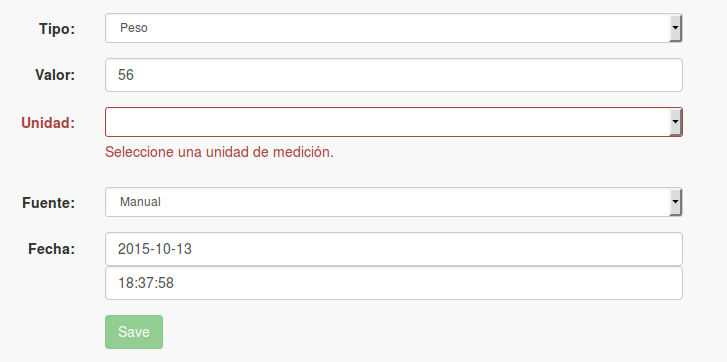
\includegraphics[width=.8\textwidth]{img/3-selecciona_tipo}
  \caption{Mensaje sutil que solicita que se seleccione un tipo de medición }
  \label{msj_seleccione_tipo}
\end{figure}

\begin{figure}[h!]
  \centering
  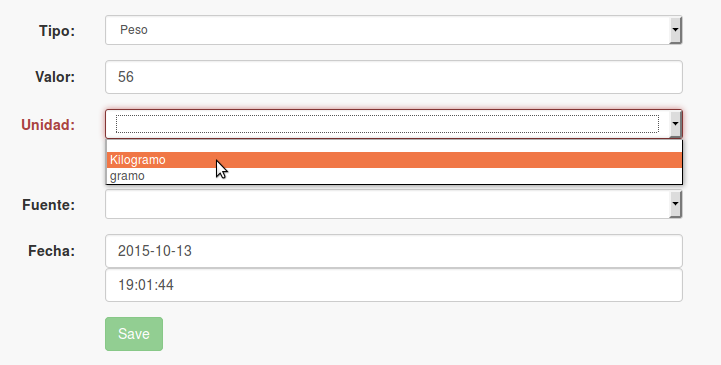
\includegraphics[width=.8\textwidth]{img/3-unidad_peso}
  \caption{Lista de unidades al seleccionar el tipo de unidad ``Peso''}
  \label{unidad_peso}
\end{figure}

 \begin{figure}[h!]
  \centering
  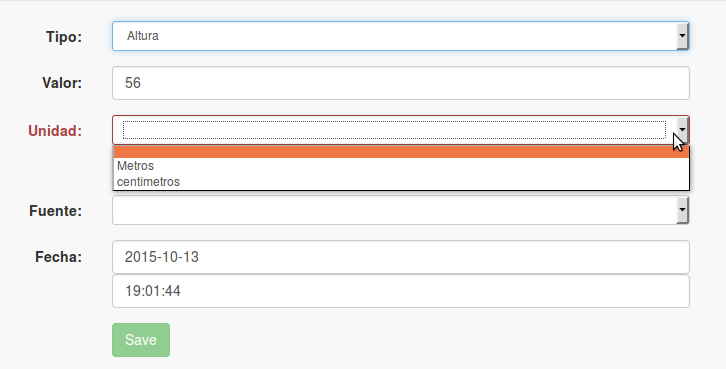
\includegraphics[width=.8\textwidth]{img/3-unidad_altura}
  \caption{Lista de unidades al seleccionar el tipo de unidad ``Altura''}
  \label{unidad_altura}
\end{figure}


El diagrama de clases, las relaciones y los recursos de la API necesarios para poder establecer esta relación se detallan en el apartado \ref{3-clases_involucradas}

\textbf{Carteles de alertas}

Luego de ejecutar las pruebas se detectó que para mejorar la experiencia del usuario es necesario añadir mensajes de avisos, como se muestra en la \textbf{Figura \ref{msj_presiona_no_escribe} y Figura \ref{msj_escribir_borrar}} indicando al usuario situaciones importantes como las que indican ausencia de información importante en el formulario, además el botón para enviar el formulario se mantiene deshabilitado hasta que se haya completado los datos obligatorios (que en este caso serían todos) del formulario.


 \begin{figure}[h!]
  \centering
  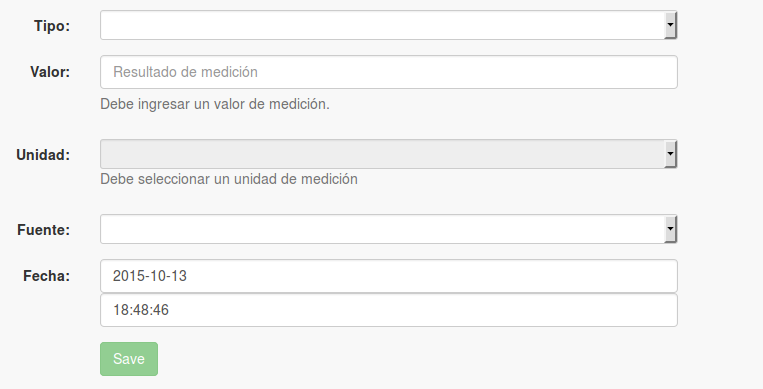
\includegraphics[width=.8\textwidth]{img/3-presiona_no_escribe}
  \caption{Mensaje sutil que aparece  si se ha presionado el campo y no se ha escrito nada}
  \label{msj_presiona_no_escribe}
\end{figure}

\begin{figure}[h!]
  \centering
  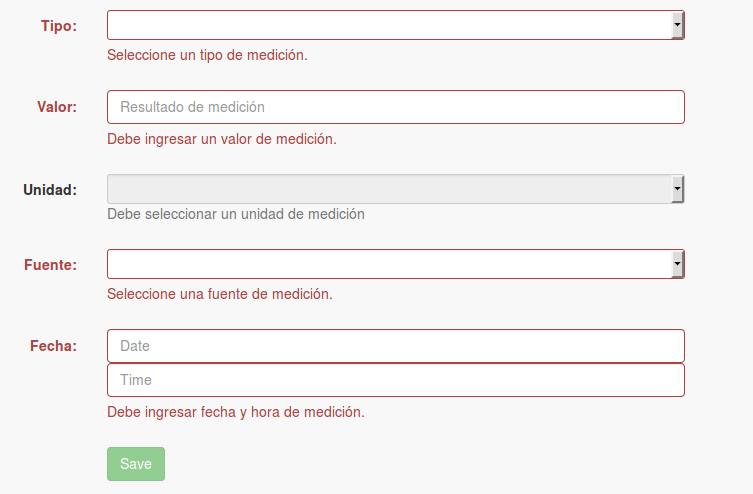
\includegraphics[width=.8\textwidth]{img/3-escribir_borrar}
  \caption{Mensaje vistoso que aparece luego de borrar lo escrito}
  \label{msj_escribir_borrar}
\end{figure}

\clearpage

\begin{lstlisting}[language=JavaScript, caption= recurso que solicita las unidades de un tipo de medición específico, label=type_unit]

 angular.module('saludWebApp')                                                   
 .factory('MeasurementTypeUnit', function (global, $resource) {                  
     // URL of specific API resource                                             
     var url=global.getApiUrl()+'/measurement_types/:id_type/units';             
                                                                                 
     return $resource( url,                                                      
         { id_type: '@_id_type' },                                                        
         { query:{method:'GET',isArray:false},                                   
           update: {method: 'PUT'}                                               
         });                                                                     
}); 
                                                                            
\end{lstlisting}



\textbf{Variable de acceso a la API global}

Fue necesario añadir  un servicio para manejar la dirección global de la API, dicho servicio se detalla en \textbf{Listing \ref{direccion_global}}
\begin{lstlisting}[language=JavaScript, caption= Servicio de la dirección global de la API, label=direccion_global]
'use strict';                                                                   
                                                                                
/**                                                                             
 * @ngdoc service                                                               
 * @name saludWebApp.global                                                     
 * @description                                                                 
 * # global                                                                     
 * Factory in the saludWebApp.                                                  
 */                                                                             
angular.module('saludWebApp')                                                   
  .factory('global', function () {                                              
    // Service logic                                                               
                                                                                
    // URL of yesdoc API                                                           
    var _api_url='https://yesdoc-api.herokuapp.com';                               
                                                                                   
    // Public methods                                                              
    return {                                                                       
      getApiUrl: function () {                                                     
        return _api_url;                                                           
      }                                                                            
    };                                                                             
  });                                                                              
~                                                                            
\end{lstlisting}


\clearpage


\subsection{Estado final de pruebas}

	\begin{itemize}
		\item \textbf{¿Qué fue bien?}
        	\begin{itemize}
				\item        Las cargas y ediciones se llevan a cabo correctamente.
			\end{itemize}

   		\item \textbf{¿Qué se mejoró?}
        	\begin{itemize}
				\item \textbf{Cerrado} Al crear una nueva medición, se mostraba un cartel (alert de javascript) con una fecha, dicho alert fue eliminado.
                \item \textbf{Cerrado} Se encontró un problema con la zona horaria que usa el servidor y la zona horaria del usuario, para solucionarlo hubo q hacer un casteo previo cuando se solicitaba la fecha y hora del usuario para mostrar.
			\end{itemize}

        	\begin{itemize}
		        \item \textbf{Cerrado} Solo debería mostrarse las unidades relacionadas al tipo de medición que se ha seleccionado 
				\item \textbf{Cerrado} En el futuro se deberá mejorar las validaciones de los datos a la hora de cargar información en los formularios.
        		\item \textbf{Cerrado} Se deberá mejorar la manera de seleccionar la fecha y la hora. 
                \item \textbf{Cerrado} Deberá realizarse los carteles de advertencia necesarios.
            \end{itemize}
       
	\end{itemize}
%%%%%%%%%%%%%%%%%%%%%%%%%%%%%%%%%%%%%%%%%%%%%%%%      FIN SPRINT 3  %%%%%%%%%%%%%%%%%%%%%%%%%%%%%%%%%%%%%%%%%%%%%%%%%%%%%%%%%%%%%%%%%%%%
\section{Sprint 4}%mostrar gráficas -validaciones
\subsection{Planificación}

\textbf{Inicio: }Martes 17 de julio del 2015 

\textbf{Fin:} Martes 11 de Septiembre del 2015

\begin{figure}[h!]
  \centering
  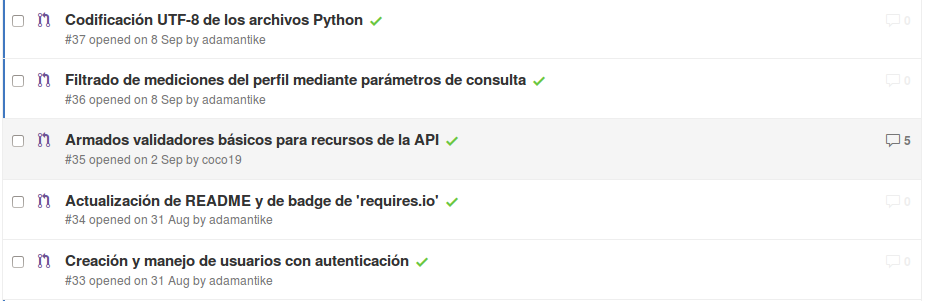
\includegraphics[width=.8\textwidth]{img/4-PR_back}
  \caption{Pull request realizados por el back end en el sprint  34}
  \label{4-PR_back}
\end{figure}
\begin{figure}[h!]
  \centering
  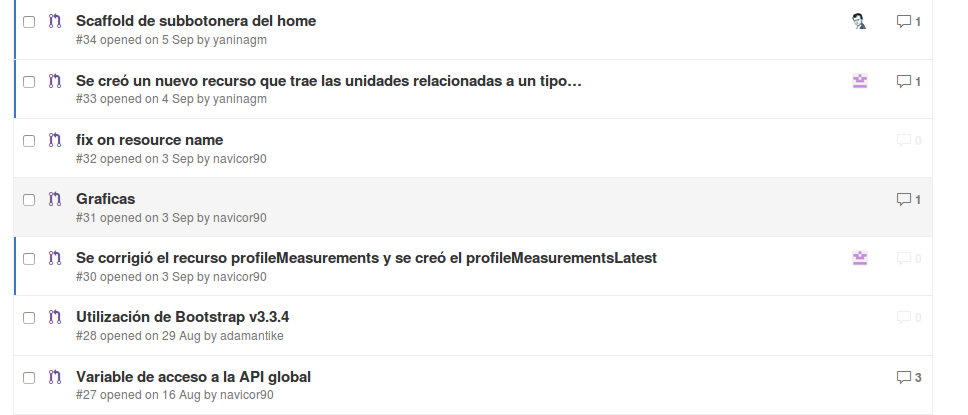
\includegraphics[width=.8\textwidth]{img/4-PR_front}
  \caption{Pull request realizados por el front end en el sprint  3}
  \label{4-PR_front}
\end{figure}

	{\scriptsize
	\begin{center} %sidewaystable
	\centering
	%\begin{adjustbox}{max width=\textheight}
    \resizebox{\textwidth}{!}
    {
	\begin{tabular}{|l|l|l|p{5cm}|l|p{1cm}|}
		\hline
		\textbf{Area a cargo} &
		\textbf{Responsable} &        
		\textbf{Revisor} &        	        
		\textbf{Tarea} &
		\textbf{US} &
		\textbf{Tiempo dedicado} \\
   		\hline
       
	    Back-end& Franco Canizo& Michael Manganiello & Agrega a la estructura de la API paquete para validadores generales.  & US-\ref{resumenInfo} \& US-\ref{infoSalud}& 8hs\\ \hline
	    Back-end& Franco Canizo& Michael Manganiello & Creación de validadores para números enteros positivos, fecha, fecha-hora, fecha-hora previa, string con\/sin números  & US-\ref{resumenInfo} \& US-\ref{infoSalud} &8hs\\ \hline
	    Back-end& Michael Manganiello& Franco Canizo & filtrado de mediciones en base al tipo, fuente y unidad de medición & US-\ref{resumenInfo} \& US-\ref{infoSalud}&9hs \\ \hline
	    Back-end& Michael Manganiello& Franco Canizo & Corrección error de comparación de fechas con información de zona horaria y fechas sin esa información & US-\ref{resumenInfo} \& US-\ref{infoSalud} &8hs\\ \hline
	    Back-end& Michael Manganiello& Franco Canizo & Simplificación del parseo de argumentos date y datetime & US-\ref{resumenInfo} \& US-\ref{infoSalud} &5hs \\ \hline        
   	    Front-end& Ivan Terreno & & Capacitación en D3 & \textbf{US-17} \& \textbf{US-15}&18hs\\ \hline
   	    Front-end& Ivan Terreno& Michael Manganiello & Generación de gráficas & \textbf{US-\ref{graficaParaPaciente}} \& \textbf{US-15}&18hs\\ \hline        
	    \end{tabular}
        }
	    %\end{adjustbox}
    	\end{center}
	}


\subsection{Descripción}
%%Descripción de Franco de validadores

Además se describirán las tareas realizadas para realizar las gráficas de las distintas mediciones

\subsection{User Stories relacionados}
La \textbf{Tabla \ref{US-Sprint4} } indicará las características de cada user story para guiarnos en el desarrollo del sprint.

\begin{table}[h]
    \label{US-Sprint4}
	%\resizebox{\textwidth}{!}{
    \centering
	\begin{tabular}{|l|p{14cm}|}
	\hline
        \multicolumn{1}{|c|}{\textbf{ID}} &
        \multicolumn{1}{|c|}{\textbf{Enunciado de la historia}} \\          
    \hline
       \ref{infoSalud} &
       Como paciente quiero cargar mi información personal de salud referido a mediciones (altura, grasa corporal, peso, presión arterial), para que el médico cuente con más y mejor información al momento de realizar el diagnóstico. 
    
       
       \\
       \hline
	    \ref{graficaParaPaciente} &
	    Como paciente quiero ver gráficas que resuman mi información en particular para poder ver mis cambios a lo largo de la historia. 

	    
	    \\
	    \hline
	    \ref{resumenInfo} &
	    Como paciente quiero obtener un resumen de mi información de salud básica para hacer uso de la misma en caso de una emergencia. 

	    
	    \\
	   \hline      
        \ref{graficaParaMedico} & Como médico quiero ver gráficas que resuman la información de un paciente para poder ver sus cambios a lo largo de la historia y así apoyar la toma de decisiones y el diagnóstico.\\
    \hline
    \end{tabular}
%     }

\end{table}

\subsection{Modelo funcional} 
Se describirán las funciones usando como marco de apoyo el sprint Backlog,
además se armará el diagrama de casos de uso del presente Sprint [Figura 44] que
irá creciendo medida se vaya avanzando en el proyecto.

\begin{comment}
	Faltaría diagrama de casos de uso para esta parte.
\end{comment}


\begin{comment}
\subsubsection{Creación de página de mediciones}
\end{comment}

\subsubsection{Validadores}
Del lado del backend el trabajo consistió en la definición de validadores usados para controlar errores y, de ser posible, sanear los datos que envían las representaciones a los recursos. Lo que se hizo es definir en un paquete una serie de validadores generales usados en el paquete \textbf{parsers} el cual se encuentra en \textbf{common}. Como podemos apreciar en la definición del parser usado por el recurso de mediciones:

\begin{lstlisting}[language=Python]
parser = reqparse.RequestParser()
parser.add_argument('datetime', type=is_valid_previous_datetime, required=True)
parser.add_argument('value', type=float, required=True)
parser.add_argument('analysis_id', type=is_valid_id, required=True)
parser.add_argument('profile_id', type=is_valid_id, required=True)
parser.add_argument('measurement_source_id', type=is_valid_id)
parser.add_argument('measurement_type_id', type=is_valid_id, required=True)
parser.add_argument('measurement_unit_id', type=is_valid_id, required=True)
\end{lstlisting}

Se define en el argumento type el llamado a una función is\_valid\_previous\_datetime, está función está definida en el paquete validators en el archivo generic validators.

\begin{lstlisting}[language=Python]
    datetime_var = is_valid_datetime(var)
    if datetime_var.year < 1900:
        raise ValueError("La fecha y hora ingresada no puede ser anterior al anio 1900.")
    elif datetime_var > datetime.utcnow():
        raise ValueError("La fecha y hora ingresada no debe ser posterior a la fecha y hora actual.")
    else:
        return datetime_var
\end{lstlisting}

Este a su vez llama al validador is\_valid\_datetime para controlar que el dato ``datetime'' tenga un valor de fecha-hora correcto. Si el validador no encuentra error devuelve la fecha-hora, en caso contrario lanza un error.
En este parser también se define un método para controlar que el id recibido es valido, por el momento lo que hace este es controlar que el id recibido sea positivo.
\begin{comment}
	Se podría poner como cosas a mejorar la validación de id.
\end{comment}

\subsubsection{Filtrado de mediciones}
El backend identifica como útil la definición de un recurso que permita devolver medidas de un perfil específico filtradas según tipo, fuente y unidad de medida. Para esto se agregó un recurso \/profile\/id\/measurements en el archivo principal de la aplicación y un recurso que define un método get para responder a una solicitud HTTP con operador GET. El mismo utiliza los datos recibidos en el ``query string'' de la URL para determinar según que tipo, fuente o unidad de medida debe filtrar. El recurso en sí no se encarga del filtrado sino que toma los datos verificados por el parse, obtiene los datos del query string y pasa estos datos a un método auxiliar definido en el archivo measurement del paquete persistence de la API ``get\_by\_profile'' el cual devuelve todas las instancias existentes de medición, asociadas a un perfil específico, ordenadas por fecha y hora de la medición, y filtradas por fuente, tipo y unidad de medición. Una vez recibida la respuesta arma el response con el código de estado correspondiente y en el cuerpo los datos resultantes serializados de acuerdo a la representación utilizada.



\subsubsection{gráficas}
Para las gráficas se utilizo D3, fue necesario añadir código javascript, el cual fue añadido con grunt
\subsection{Salidas del sistema}
El resultado de la implementación del código necesario para mostrar las gráficas del peso se puede ver en la \textbf{[Figura \ref{5-grafica_medicion}]}, 


\begin{figure}[h!]
  \centering
  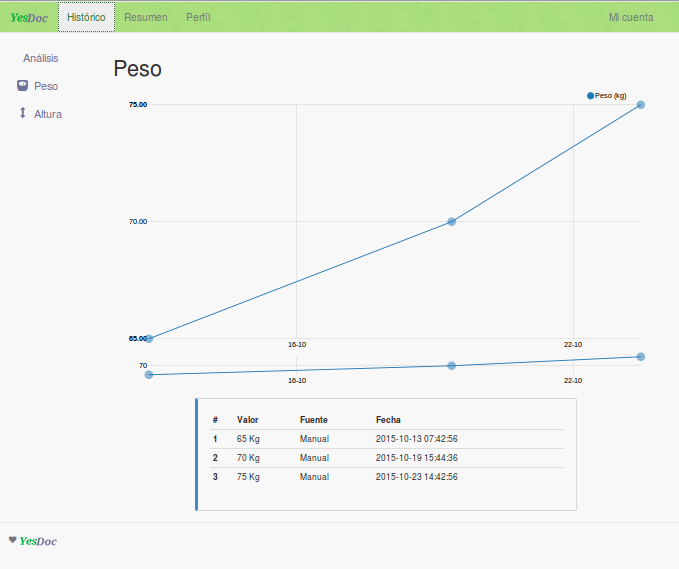
\includegraphics[width=.8\textwidth]{img/5-grafica_medicion}
  \caption{vista generada para una medición en particular}
  \label{5-grafica_medicion}
\end{figure}


\begin{comment}
	Faltaría agregar algunas pruebas con curl y algo de código.
    Poner que se desarrollo para pasar datos específicos para que el front-end presente datos resumidos cuando estos son muchos y complejos??
\end{comment}

\subsection{Criterios de aceptación}

\begin{center}
\begin{longtable}{|p{0.5cm}|p{4cm}|p{4cm}|p{5cm}|}
\hline \hline \rowcolor[gray]{0.9}
	\multicolumn{4}{||c|}{\textbf{Criterio de aceptación}} \\
    \hline  \rowcolor[gray]{0.9}
        \textbf{Id} &
        \textbf{Contexto} &
        \textbf{Evento}&
        \textbf{Resultado} \\
    \hline
1&En caso de que se envíe como id un valor menor o igual a 0 en cualquier representación  de una solicitud & Al ejecutar el método post, get, delete o put correspondiente del recurso & El sistema devolverá un json con el mensaje de error por entero no positivo y el código de error 400 \\ \hline
	\hline
2&En caso de que se indique una fecha cuyo año sea menor a 1900 & al ejecutar el validador is\_valid\_previous\_date del argumento  & El sistema devolverá un json con el mensaje de error correspondiente a una fecha previa no permitida y el código de estado 400 \\ 		\hline
	\hline
3&En caso de que se indique en la solicitud una fecha-hora con formato invalida 
& Al ejecutar el validador \textbf{ is\_valid\_datetime}  & El sistema devolverá un json con el mensaje de error correspondiente a una fecha hora con formato inválido y el código de estado 400\\ \hline
    \hline
4&En caso de que no exista un usuario registrado con el id indicado & al ejecutar el método get\/put del recurso \/users\/id  & El sistema devolverá un json con un mensaje de error y un código de error 404 \\ \hline
	\hline
5&En caso de que no exista un perfil registrado con el id indicado & al ejecutar el método get del recurso \/profile\/id\/measurements  & El sistema devolverá un json con un mensaje de error por no encontrar la instancia correspondiente \\ \hline

  \end{longtable}
\end{center}

\begin{comment}
	Cuando paso un entero no positivo no responde con error sino que query or get 404 no encuentra el registro.
    El método get_latest_by_profile es del sprint2 cierto?
\end{comment}

\subsection{Pruebas ejecutadas}
A continuación se detalla la situación en la que quedaron las pruebas ejecutadas en los sprint anteriores, luego se desarrollarán las soluciones que se usaron y por última se cambiará el estado de aquellas errores encontrados por \textit{"cerrado"}.
        %
	\begin{itemize}
		\item \textbf{¿Qué fue bien?}
        	\begin{itemize}
				\item        Las cargas y ediciones se llevan a cabo correctamente.
			\end{itemize}

   		\item \textbf{¿Qué se mejoró?}
        	\begin{itemize}
				\item \textbf{Cerrado} Al crear una nueva medición, se mostraba un cartel (alert de javascript) con una fecha, dicho alert fue eliminado.
                \item \textbf{Cerrado} Se encontró un problema con la zona horaria que usa el servidor y la zona horaria del usuario, para solucionarlo hubo q hacer un casteo previo cuando se solicitaba la fecha y hora del usuario para mostrar.
			\end{itemize}

   		\item \textbf{¿Qué se puede mejorar?}
        	\begin{itemize}
		        \item \textbf{Abierto} Solo debería mostrarse las unidades relacionadas al tipo de medición que se ha seleccionado 
				\item \textbf{Abierto} En el futuro se deberá mejorar las validaciones de los datos a la hora de cargar información en los formularios.
        		\item \textbf{Abierto} Se deberá mejorar la manera de seleccionar la fecha y la hora. 
                \item \textbf{Abierto} Deberá realizarse los carteles de advertencia necesarios.
            \end{itemize}
       
	\end{itemize}



\subsection{Estado final de pruebas}

	\begin{itemize}
		\item \textbf{¿Qué fue bien?}
        	\begin{itemize}
				\item        Las validaciones.
			\end{itemize}
            
		\item \textbf{¿Qué fue mal?}
        	\begin{itemize}
				\item        La librería que se utilizó al principio ``lvd3'' era de muy bajo nivel, por ello tuvo q cambiarse a D3 que es de más alto nivel. 
			\end{itemize}
            
   		\item \textbf{¿Qué se mejoró?}
        	\begin{itemize}
            	\item \textbf{Cerrado} Mal rendimiento de D3, mejorado usando código de la libreria lvd3
            	\item \textbf{Cerrado} Función de maximizar
                \item \textbf{Cerrado} Facilitar el pasaje del scope al controlador
                \item \textbf{Cerrado} Se encontró un problema con la zona horaria que usa el servidor y la zona horaria del usuario, para solucionarlo hubo q hacer un casteo previo cuando se solicitaba la fecha y hora del usuario para mostrar.
			\end{itemize}
       
	\end{itemize}

%%%%%%%%%%%%%%%%%%%%%%%%%%%%%%%%%%%%%%%%%%%%%%%%%%%%%%%%%%%%%%%%%%%%%%      FIN SPRINT 4  %%%%%%%%%%%%%%%%%%%%%%%%%%%%%%%%%%%%%%%%%%%%%%%%%%%%%%%%%%%%%%%%%%%%%%%%%%%%%%%%%%%%%%%%%%%

\section{Sprint 5}%Autenticación
\subsection{Planificación}

	\textbf{Inicio: } 10 de Septiembre del 2015
	
	\textbf{Fin:} 27 de Septiembre del 2015 



\subsection{Descripción}

Este sprint tiene por objetivo definir un proceso de autenticación del usuario para con la API, sin importar el perfil del mismo, que garantice un nivel de seguridad adecuado para tranquilidad en el uso de la aplicación por parte de los interesados. 

\subsection{User Stories relacionados}
La \textbf{Tabla \ref{US-Sprint5} } indicará las características de cada user story para guiarnos en el desarrollo del sprint.
\begin{comment}
	como usuario quiero contar con un acceso único y privado a mi información. Agregaría este user story, habría que ver la traza con el documento de diseño para que queden balanceados.
\end{comment}
\begin{table}[h]
    \label{US-Sprint5}
	%\resizebox{\textwidth}{!}{
    \centering
	\begin{tabular}{|l|p{9cm}|}
	\hline
        \multicolumn{1}{|c|}{\textbf{ID}} &
        \multicolumn{1}{|c|}{\textbf{Enunciado de la historia}} \\          
    \hline
        \textbf{US-\ref{modificarPermisos}} & Como paciente, quiero modificar los permisos de visualización de mis datos con respecto a cada uno de los integrantes de grupo familiar para tener un control total sobre mi privacidad. \\
     \hline 
        \textbf{US-\ref{validarUsuario} } & Como usuario quiero contar con un acceso único y privado a mi información. \\
     \hline 
     
    \end{tabular}
%     }

\end{table}
\subsection{Modelo de datos}
El Diagrama propio de este sprint se puede ver en la \textbf{Figura\ref{5-clase_autenticacion}}, allí se indican exactamente las clases que se usarán en este sprint y que serán detalladas con detenimiento en el presente documento. 

\begin{figure}[h]
        \centering
        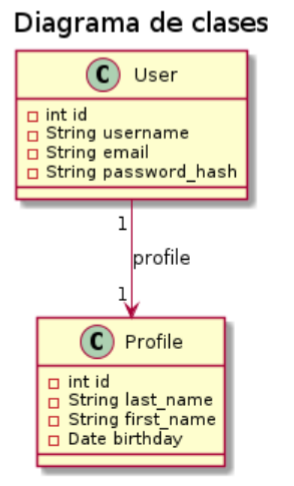
\includegraphics[width=0.3\textwidth]{img/clases_auth}
        \caption{Diagrama de clases autenticación.}
		\label{5-clase_autenticacion}
    \end{figure}

\subsection{Modelo funcional} 
Se define el diagrama de casos de uso del presente Sprint \textbf{[Figura \ref{4-cu_autenticacion}]}.

    \begin{figure}[h]
        \centering
        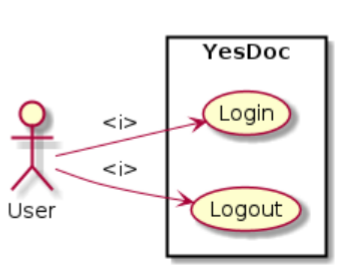
\includegraphics[width=0.4\textwidth]{img/cu_autenticacion}
        \caption{Casos de uso autenticación}
		\label{4-cu_autenticacion}
    \end{figure}

	{\scriptsize
	\begin{center} %sidewaystable
	\centering
	%\begin{adjustbox}{max width=\textheight}
    \resizebox{\textwidth}{!}{
		\begin{tabular}{|l|l|l|p{5cm}|l|p{1cm}|}
			\hline
			\textbf{Area a cargo} &
			\textbf{Responsable} &        
			\textbf{Revisor} &        	        
			\textbf{Tarea} &
			\textbf{US} &
			\textbf{Tiempo dedicado} \\
			\hline
			
	    Backend& Michael Manganiello& Franco Canizo & Generación del modelo User y relación del mismo con el modelo Profile.  & US-\ref{modificarPermisos} \& US-\ref{validarUsuario} & 13hs
	     \\ \hline
	    Backend& Michael Manganiello& Franco Canizo & Generación del recurso relacionado con el modelo User y los métodos post y get que manejan los operadores HTTP correspondientes.  & US-\ref{modificarPermisos} \& US-\ref{validarUsuario} & 11hs
	    \\ \hline
	    Backend& Michael Manganiello & Franco Canizo& Generación del recurso para obtener un token para un usuario autenticado.  & US-\ref{modificarPermisos} \& US-\ref{validarUsuario} &9hs
	    \\ \hline
		Backend& Michael Manganiello & Franco Canizo& Se creó el recurso /my/profile, que hace uso de la autenticación para obtener la información del perfil asociado al usuario. Permite los métodos GET y PUT. & US-\ref{modificarPermisos} \& US-\ref{validarUsuario} & 4hs
		\\ \hline
		Backend& Michael Manganiello & Franco Canizo& Se crearon dos nuevos recursos GET:
		\begin{itemize}
			\item 		/my/measurements
			\item		/my/measurements/latest
		\end{itemize}
		Ambos recursos requieren autenticación (ya sea mediante usuario y contraseña, o token de sesión) y retornan las mediciones asociadas al perfil del usuario autenticado. Por lo tanto, no es necesario especificar un id de perfil, sino que se toma el perfil del usuario que realiza la petición. & US-\ref{modificarPermisos} \& US-\ref{validarUsuario} & 8hs
		\\ \hline
		Frontend& Yanina Morales  & Ivan Terreno& Se cambiaron las referencias a los recursos para utilizar los que requieren que el usuario se encuentre logueado & US-\ref{modificarPermisos} \& US-\ref{validarUsuario} & 12hs
		\\ \hline
		Frontend& Yanina Morales  & Ivan Terreno& Se corrigieron errores para que el navbar sea responsive & US-\ref{modificarPermisos} \& US-\ref{validarUsuario} & 8hs
		\\ \hline		
	    \end{tabular}
        }
	    %\end{adjustbox}
    	\end{center}
	}
    
\subsubsection{Definición de modelos}
La definición del modelo User es bastante compleja ya que define métodos para tomar la password  y guardarla como un hash, a su vez, puede recibir passwords encriptadas y desencriptarlas. Por otro lado, define métodos para la generación y verificación del token asignado al usuario. Por último, define una relación uno a uno con el modelo Profile.

\subsubsection{Recursos}
El desafío en cuanto a la definición de recursos radica en que según lo que establece REST, la restricción de que la API debe ser stateless invalida la posibilidad de usar sesiones para que la API sea escalable, es por esto que definimos una solución que se presenta en un punto gris entre puristas de REST y quienes realmente no hacen REST. La solución consiste en generar un token para el usuario autenticado el cual se almacena en las cookies y es usado en cada solicitud para autenticar al usuario. Por esto se definen recursos para dar de alta al usuario y para entregarle un token.

	\begin{lstlisting}[language=Python]
	api.add_resource(UserView, '/users/<int:id>')
	api.add_resource(UserList, '/users')
	api.add_resource(Token, '/token')
	api.add_resource(MyUserView, '/my/user')
	\end{lstlisting}

\subsection {Salidas del Sistema}

\begin{enumerate}
	\item \textbf{Solicitud post al recurso del perfil}
    
	Para crear un usuario debe existir un perfil creado, para esto usamos el recurso ``\/profiles'' a través del método POST y pasando como argumento los datos first\_name, last\_name, birthday y gender\_id.
    \item \textbf{Solicitud post al recurso del user}
    
    Realizamos ahora una solicitud HTTP, con método post utilizando curl al recurso del usuario usando el id del perfil creado previamente:

\begin{verbatim}
curl -i http://localhost:5000/users -H "Content-Type: 
application/json" -X POST -d '{"username":"akathy", 
"email":"kathy@gmail.com", "password":"kathy1234", 
"profile_id":"2"}'
\end{verbatim}
    
    Obtenemos la siguiente respuesta de la API, con un código 201.
    
\begin{lstlisting}[language=json]
HTTP/1.0 201 CREATED
Content-Type: application/json
Content-Length: 425
Server: Werkzeug/0.10.4 Python/2.7.6
Date: Tue, 20 Oct 2015 05:21:37 GMT

{
    "resource": {
        "email": "kathy@gmail.com", 
        "id": 2, 
        "profile": {
            "birthday": "1989-06-17", 
            "first_name": "Katherina", 
            "gender": {
                "description": "female gender", 
                "id": 2, 
                "name": "female"
            }, 
            "id": 2, 
            "last_name": "Aguirre"
        }, 
        "username": "akathy"
    }
}
\end{lstlisting}

    \item \textbf{Solicitud post al recurso token usando user y password}
    
    Luego con este usuario y contraseña solicitamos un token al recurso correspondiente:

\begin{verbatim}
curl -u akathy:kathy1234 http://localhost:5000/token
\end{verbatim}
   
   Obtenemos así el token que debe ser almacenado en las cookies, tendrá una duración de 10 minutos y será utilizado en cada solicitud para autenticación.
   
\begin{lstlisting}[language=json]
{
    "resource": {
        "duration": 600, 
        "token": "eyJhbGciOiJIUzI1NiIsImV4cCI6MTQ0NTMxOTM3MCwiaWF0IjoxNDQ1MzE4NzcwfQ.eyJpZCI6Mn0.2eZRjbMq9tg4GykJx8EU-Ux4ZoyUW6WnBlADsvnpQvE"
    }
}
\end{lstlisting}

\end{enumerate}

\clearpage
\subsection{Criterios de aceptación}

\begin{center}
\begin{longtable}{|p{0.5cm}|p{4cm}|p{4cm}|p{5cm}|}
\hline \hline \rowcolor[gray]{0.9}
	\multicolumn{4}{||c|}{\textbf{Criterio de aceptación}} \\
    \hline  \rowcolor[gray]{0.9}
        \textbf{Id} &
        \textbf{Contexto} &
        \textbf{Evento}&
        \textbf{Resultado} \\
    \hline
1&En caso de que exista un usuario registrado con el mismo username & al ejecutar el método post del recurso \/users  & El sistema devolverá un json vacío y un código de error 400 \\ \hline
	\hline
2&En caso de que exista al menos un usuario registrado & al ejecutar el método get del recurso \/users  & El sistema devolverá una lista de json con los datos de los users registrados \\ 		\hline
	\hline
3&En caso de que exista un usuario registrado con el mismo username & al ejecutar el método post del recurso \/users  & El sistema devolverá un json vacío y un código de error 400 \\ \hline
    \hline
4&En caso de que no exista un usuario registrado con el id indicado & al ejecutar el método get\/put del recurso \/users\/id  & El sistema devolverá un json con un mensaje de error y un código de error 404 \\ \hline

  \end{longtable}
\end{center}

\begin{comment}
	Cuando devolvería 401 el recurso del token.
\end{comment}

\subsection{Casos de prueba}

\subsubsection{Pruebas de integración entre módulos del Sistema}

\subsubsection{Pruebas de carga}

\subsubsection{Pruebas de seguridad por niveles de usuarios}


\subsection{Pruebas ejecutadas}
Aqui se realizará una conclusión general de lo que se descubrió en las pruebas.
        %
	\begin{itemize}
		\item \textbf{¿Que fue bien?}
        	\begin{itemize}
				\item        Las cargas y ediciones se llevan a cabo correctamente.
			\end{itemize}

   		\item \textbf{¿Que se mejoró?}
        	\begin{itemize}
                \item \textbf{Cerrado} problema
			\end{itemize}

   		\item \textbf{¿Que se puede mejorar?}
        	\begin{itemize}
		        \item \textbf{Abierto} En el futuro se deberá mejorar ...
            \end{itemize}
        

	\end{itemize}

%%%%%%%%%%%%%%%%%%%%%%%%%%%%%%%%%%%%%%%%%%%%%%%%%%%%%%%%%%%%%%%%    FIN SPRINT 5    %%%%%%%%%%%%%%%%%%%%%%%%%%%%%%%%%%%%%%%%%%%%%%%%%%%%%%%%%%%%%%%




\section{Sprint 6} % MOSTRAR, CARGAR Y EDITAR ANÁLISIS
\subsection{Planificación}

\textbf{Inicio:  } 27 de septiembre del 2015

\textbf{Fin: } 17 de octubre del 2015

\begin{figure}[h!]
  \centering
  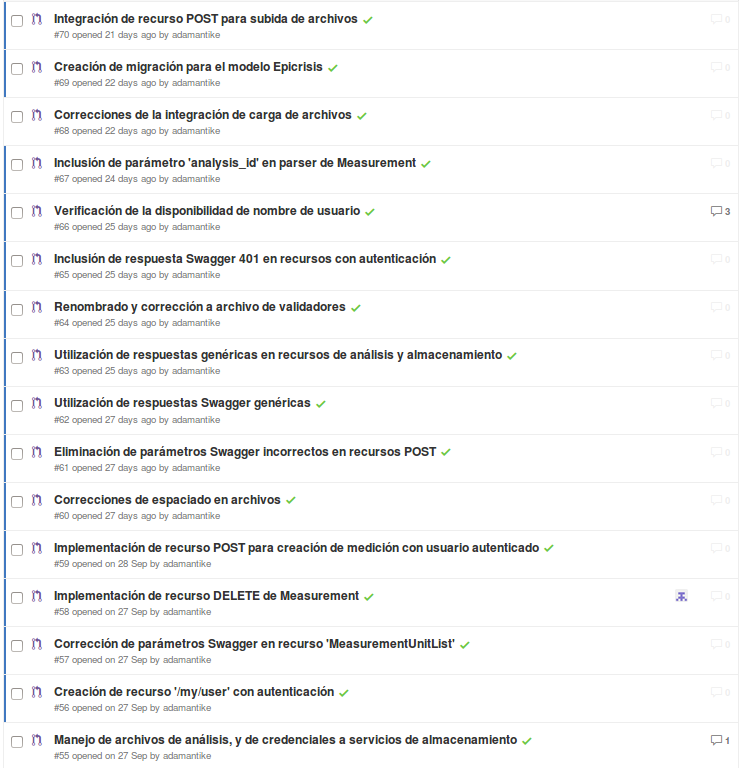
\includegraphics[width=.5\textwidth]{img/6-PR_1}
  \caption{Pull request realizados en el sprint  6}
  \label{6-PR_1}
\end{figure}

\begin{figure}[h!]
	\centering
	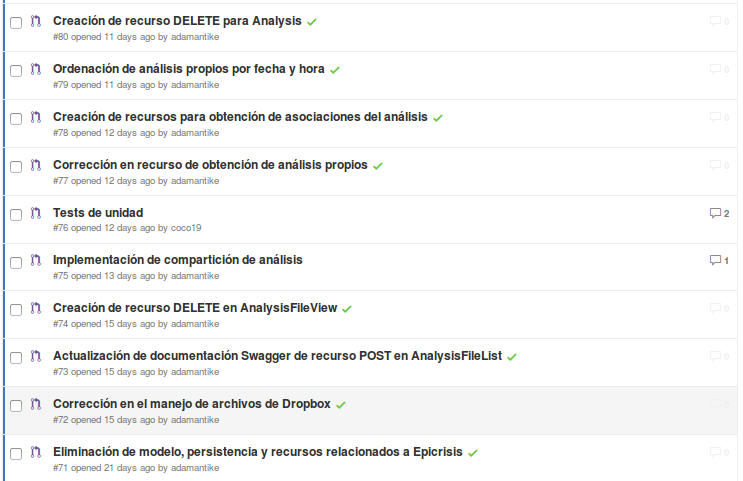
\includegraphics[width=.8\textwidth]{img/6-PR_2}
	\caption{Pull request realizados en el sprint 6}
	\label{6-PR_1}
\end{figure}
\clearpage



{\scriptsize
	\begin{center} %sidewaystable
		\centering
		%\begin{adjustbox}{max width=\textheight}
		\resizebox{\textwidth}{!}{
			\begin{tabular}{|l|p{3cm}|l|p{6cm}|p{2cm}|p{1cm}|}
				\hline
				\textbf{Area a cargo} &
				\textbf{Responsable} &   
             	\textbf{Revisor} &      
				\textbf{Tarea} &
				\textbf{US} &
				\textbf{tiempo dedicado}\\
				\hline
				Front-end& Ivan Terreno & Yanina Morales & Diseño de Interface de epicrisis 
				& \textbf{US-\ref{infoPaciente}} \& \textbf{US-\ref{cargaCentroSalud}} \&\textbf{US-\ref{infoSalud}}\& \textbf{US-\ref{evitarPerdidas} } 
				 & 8 hs
				\\ \hline
				
				
				Front-end& Ivan Terreno & Michael Manganiello & Enlazado de interfaces ya existentes de mediciones con la nueva interfaz & \textbf{US-\ref{infoPaciente}} \& \textbf{US-\ref{cargaCentroSalud}} \&\textbf{US-\ref{infoSalud}}\& \textbf{US-\ref{evitarPerdidas} }
				 & 3hs 
				\\ \hline
				
				Front-end& Ivan Terreno & Michael Manganiello & Creación de los recursos que consumirán la información de la API &
				  \textbf{US-\ref{infoPaciente}} \& \textbf{US-\ref{cargaCentroSalud}} \&\textbf{US-\ref{infoSalud}}\& \textbf{US-\ref{evitarPerdidas} } 
				&
				3 hs
				\\ \hline
				
				Front-end& Ivan Terreno Yanina Morales&  & Búsqueda de iconos representativos& 
				\textbf{US-\ref{infoPaciente}} \& \textbf{US-\ref{cargaCentroSalud}} \&\textbf{US-\ref{infoSalud}}\& \textbf{US-\ref{evitarPerdidas} } 
				& 1hs
				\\ \hline
				
				Front-end& Ivan Terreno & Yanina Morales & Detección de tipo de archivo& 
				\textbf{US-\ref{infoPaciente}} \& \textbf{US-\ref{cargaCentroSalud}} \&\textbf{US-\ref{infoSalud}}\& \textbf{US-\ref{evitarPerdidas} } 
				 & 5hs
				\\ \hline   
				     
				     
				Front-end& Ivan Terreno& Michael Manganiello &  Carga de archivos,por POST & 
				\textbf{US-\ref{infoPaciente}} \& \textbf{US-\ref{cargaCentroSalud}} \&\textbf{US-\ref{infoSalud}}\& \textbf{US-\ref{evitarPerdidas} } 
				 & 4hs
				 \\ \hline 
				       
				       
				Front-end& Ivan Terreno& Michael Manganiello &  funcionalidad de editar y ver archivos y análisis &\textbf{US-\ref{infoPaciente}} \& \textbf{US-\ref{cargaCentroSalud}} \&\textbf{US-\ref{infoSalud}}\& \textbf{US-\ref{evitarPerdidas} } 
				 & 6hs
				\\ \hline
				
				
				Back end& Michael Manganiello & Ivan Terreno& Creación de nueva clase Analysis del modelo, y adaptación de las existentes. &
				\textbf{US-\ref{infoPaciente}} \& \textbf{US-\ref{cargaCentroSalud}} \&\textbf{US-\ref{infoSalud}}\& \textbf{US-\ref{evitarPerdidas} } 
				 & 6hs
				\\ \hline
				
				
				
				Back end& Michael Manganiello & Franco Canizo& Creación de recurso ``/my/analyses'', con métodos GET y POST & \textbf{US-\ref{infoPaciente}} \& \textbf{US-\ref{cargaCentroSalud}} \&\textbf{US-\ref{infoSalud}}\& \textbf{US-\ref{evitarPerdidas} } 
				& 6hs
				\\ \hline   
				
				      
				Back end& Michael Manganiello & Ivan Terreno& Se crean los recursos GET necesarios para obtener las mediciones asociaciadas a un determinado análisis & \textbf{US-\ref{infoPaciente}} \& \textbf{US-\ref{cargaCentroSalud}} \&\textbf{US-\ref{infoSalud}}\& \textbf{US-\ref{evitarPerdidas} } 
				& 6hs
				\\ \hline   
				     
				      
				      
				Back end& Michael Manganiello& Yanina Morales & Se ordenan los análisis devueltos por el recurso GET en /my/analysis, por fecha y hora, en forma ascendente (de más antiguo a más actual) & \textbf{US-\ref{infoPaciente}} \& \textbf{US-\ref{cargaCentroSalud}} \&\textbf{US-\ref{infoSalud}}\& \textbf{US-\ref{evitarPerdidas} } 
				 & 6hs
				\\ \hline 
				
				
				Back end& Michael Manganiello& Franco canizo & Se corrige el uso de backref entre clases & \textbf{US-\ref{infoPaciente}} \& \textbf{US-\ref{cargaCentroSalud}} \&\textbf{US-\ref{infoSalud}}\& \textbf{US-\ref{evitarPerdidas} } 
				& 6hs
				\\ \hline
				
				
			\end{tabular}
		}
		%\end{adjustbox}
	\end{center}
}


\subsection{Descripción}
%navbar responsive

	La carga de medidas de salud permite a los usuarios tanto médico como paciente un seguimiento de su estado, sin embargo estas mediciones no deben existir aisladas. La definición de un análisis permite al usuario reunir una serie de mediciones y darles un motivo que destaque la razón por la cual se tomó dicha medida. Así un usuario podría indicar el análisis que reúne las medidas diarias de presión o las medidas de presión, peso y azúcar que forman parte de los controles diarios que se realiza un usuario. Por otro lado un médico puede ingresar el conjunto de medidas e imágenes que formaron parte del proceso de diagnóstico de una persona o el mismo paciente, una vez terminada la consulta podría crear un análisis indicando el motivo y reuniendo los resultados de mediciones tomadas manualmente. Finalmente, la definición de este análisis permite a la persona guardar una imagen con los resultados de un estudio y, posteriormente, tomar esta imagen y cargar las medidas de interés manualmente para que así YesDoc las presente de forma tal que le permita identificar una progresión en el tiempo.
	
	En este sprint se le permitirá al usuario definir un nuevo análisis indicando la fecha y hora de realización y una descripción útil para una consulta posterior del mismo. Permitirá cargar medidas manualmente y asociarlas al análisis ya sea al momento de crearlo o también post creación.
	
	Permitirá al usuario obtener todas las medidas asociadas al análisis.
	
	El usuario podrá consultar todos los análisis que le pertenecen, es decir, todos los análisis asociados a su perfil bajo algún criterio como sería los más recientes de acuerdo a la fecha de creación. 
	
	El usuario podrá actualizar y eliminar sus análisis.
	
	Este sprint se basa en el sprint2 donde se ha desarrollado la carga de mediciones.
	 

\subsection{User Stories relacionados}
%\textbf{Tabla \ref{US-Sprint6}}
La \textbf{Tabla \ref{USrelacionados-Sprint6}} indica las características de cada user story para guiarnos en el desarrollo del sprint.

\begin{table}[h]

	%\resizebox{\textwidth}{!}{
    \centering
	\begin{tabular}{|l|p{9cm}|}
	\hline
        \multicolumn{1}{|c|}{\textbf{ID}} &
        \multicolumn{1}{c|}{\textbf{Enunciado de la historia}} \\          
    \hline
        \textbf{US-\ref{evitarPerdidas} } & Como paciente, quiero añadir al sistema los estudios realizados para evitar posibles perdidas.\\
    \hline
    	\textbf{US-\ref{infoSalud}} & Como paciente quiero cargar mi información personal de salud referido a mediciones (altura, grasa corporal, peso, presión arterial), para que el médico cuente con más y mejor información al momento de realizar el diagnóstico.\\
    \hline
    \textbf{US- \ref{cargaCentroSalud}} & Como paciente quiero que los sistemas de salud existentes puedan cargar sus resultados directamente en mi carpeta de salud para centralizar mi
    información\\
    \hline
    \textbf{US-\ref{infoPaciente}} &Como laboratorio, quiero cargar información de un paciente en su cuenta para ahorrarle las molestias de volver.\\
    \hline
    \end{tabular}
%     }
    \label{USrelacionados-Sprint6}
\end{table}

\subsection{Modelo funcional} %Diagrama de clases
Se describirán las funciones usando como marco de apoyo el sprint Backlog, además se armará el diagrama de casos de uso del presente Sprint \textbf{[Figura \ref{6-cu}]} acompañado de los casos de uso que se obtuvieron como resultado de los sprint anteriores



\begin{figure}[h]
	\centering
	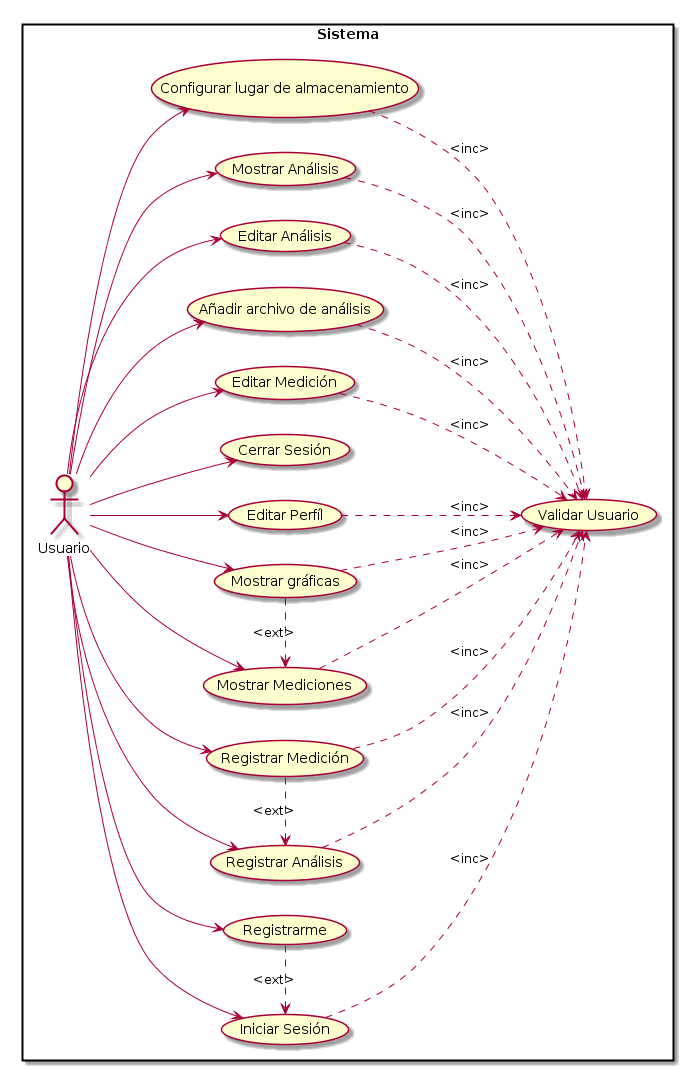
\includegraphics[width=0.6\textwidth]{img/6-cu}
	\caption{formulario de edición de perfil}
	\label{6-cu}
\end{figure}

\clearpage

\subsection{Modelo de datos}
El Diagrama propio de este sprint se puede ver en la \textbf{Figura \ref{5-diagramaClases}}, en ella se indican exactamente las clases que se usarán en este sprint. Estas clases representan un incremento en el diseño de las clases definidas en el sprint 2 de mediciones ya que unifica en un análisis todas las medidas relacionadas evitando la existencia de mediciones colgadas para las cuales no se indica una referencia que denote el motivo de la toma de dicha medición.

    \begin{figure}[h]
        \centering
        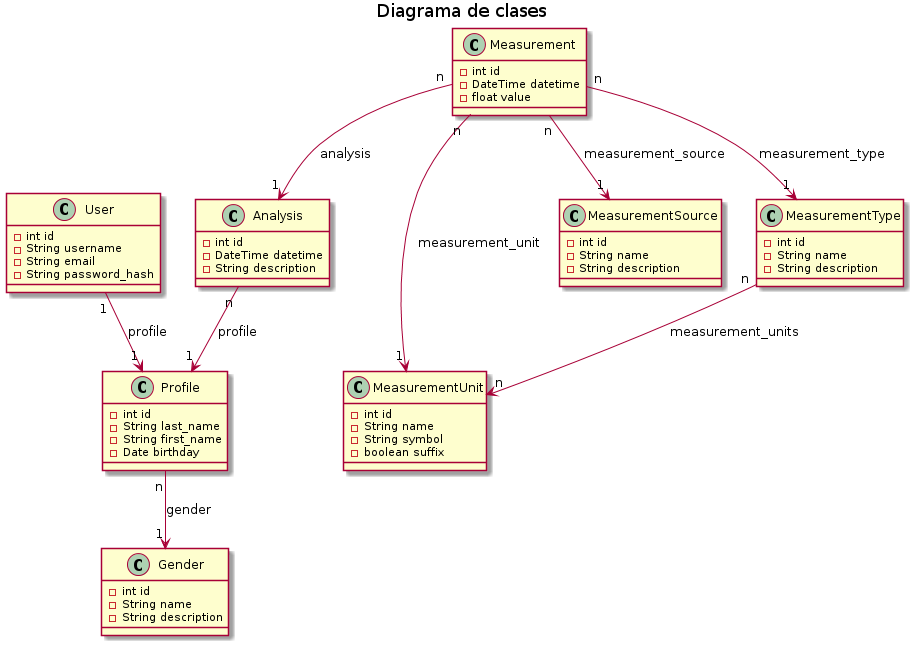
\includegraphics[width=0.8\textwidth]{img/sprint5_dc}
        \caption{Diagrama de clases referido a la carga de análisis}
		\label{5-diagramaClases}
    \end{figure}


\subsection{Diseño}

	Se define el modelo para la gestión de los análisis \textbf{Analysis} el cual presenta los siguientes \textbf{atributos}:

\begin{itemize}
	\item \textbf{id:} Identificador único del modelo.
	\item \textbf{description:} Descripción del análisis.
	\item \textbf{datetime: }	Fecha y hora de creación del análisis.	
	\item \textbf{profile\_id: } Identificador único del perfil al que pertenece el análisis.
\end{itemize}

	Este modelo presenta dos recursos que pueden ser usados por el cliente de la API, los recursos no visibles \textbf{AnalysisList} que ofrece servicios para la carga de nuevos análisis y obtener análisis cargados, \textbf{MyAnalysisList} el cual ofrece servicios para obtener todas los análisis del usuario registrado y cargar un análisis que pertenezca al usuario registrado y no pueda ser consultado por otro y el recurso \textbf{AnalysisMeasurementList} para obtener todas las medidas relacionadas a un análisis. Por otro lado tenemos un recurso visible \textbf{AnalysisView} que ofrece servicios para obtener, modificar y eliminar un análisis específico a partir de un identificador.
	
	
	Acompañando la creación de este nuevo modelo se crearon las representaciones para manejar las solicitudes y armar las respuestas de la API en los paquetes parsers el archivo \textbf{analysis.py} y en el paquete fields la clase \textbf{AnalysisFields}.
	
	Se definieron identificadores de acceso (URLs) para acceder a estos recursos desde un cliente.
		\begin{itemize}
			\item \textbf{/analysis/<int:analysis\_id>}
			\item \textbf{/analysis}
			\item \textbf{/analysis/<int:analysis\_id>/measurements}
			\item \textbf{/my/analyses}
		\end{itemize} 
		
	Por otro lado, se modificó el modelo \textbf{Measurement} para ser asociado a un análisis añadiendo el atributo relacional \textbf{analysis}. Con esta modificación se tuvo que actualizar también servicios y representaciones de los recursos que envuelven éste modelo.
	
	Finalmente se crea una nueva versión del script que carga la base de datos para cargar la tabla que mantiene los datos del análisis.

\clearpage
\subsection {Salidas del Sistema - Incrementos}

Luego de finalizado este user story se obtendrán 5 pantallas que se detallarán a continuación:
\begin{enumerate}
	\item \textbf{Vista para acceder a carga de nueva medición}: \textbf{[Figura \ref{5-boton_nuevo_analisis}]} En la imagen se muestra la forma que tiene el usuario de acceder  a realizar la carga de un análisis.
    	\item \textbf{Crear Análisis}: \textbf{[Figura \ref{5-crear_analisis}]} En la imagen se muestra el formulario que corresponde a un análisis. Por lo general los análisis son un conjunto de mediciones las cuales suelen provenir de un estudio presentada en papel. Por eso en el formulario contemplamos dos campos el de carga de mediciones y el de carga de imágenes que a continuación se detallan.
        	\item \textbf{Carga de mediciones}: \textbf{[Figura \ref{5-cargar_medicion}]} Se le permitirá cargar mediciones que realice en algún momento del día como son peso, altura, grasa corporal y glucosa. Deberá indicar la fuente, tipo, unidad y fecha de la medición. Este formulario es el mismo que el descripto en el\textbf{ Sprint 2.}
    \item \textbf{Carga de imágenes}  \textbf{[Figura  \ref{5-cargar_img} ]} Como se explicó anteriormente se le permite al usuario cargar imágenes correspondiente al estudio/análisis realizado. Cabe destacar en este punto y para los subsiguientes en los cuáles se hace mención de la "carga de archivos",  que el equipo de front end, en este sprint, trabajó con stubs para simular la carga de archivos y así poder utilizarlos con el fin de poder definir la mejor forma de mostrarlos al usuario.

    \item \textbf{Imágenes y mediciones cargadas en el formulario:}  \textbf{[Figura \ref{5-mediciones_cargadas}]} Esta interfaz destaca la funcionalidad de edición, eliminación y vista previa que brinda el formulario.

\end{enumerate}

    
    \begin{figure}[h]
        \centering
        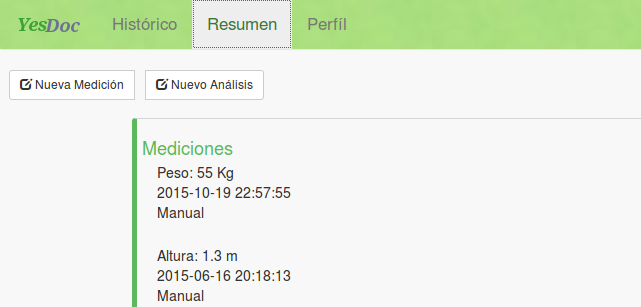
\includegraphics[width=0.5\textwidth]{img/5-boton_nuevo_analisis}
        \caption{vista para acceder a cargar nuevo análisis}
		\label{5-boton_nuevo_analisis}
    \end{figure}
    
    \begin{figure}[h]
        \centering
        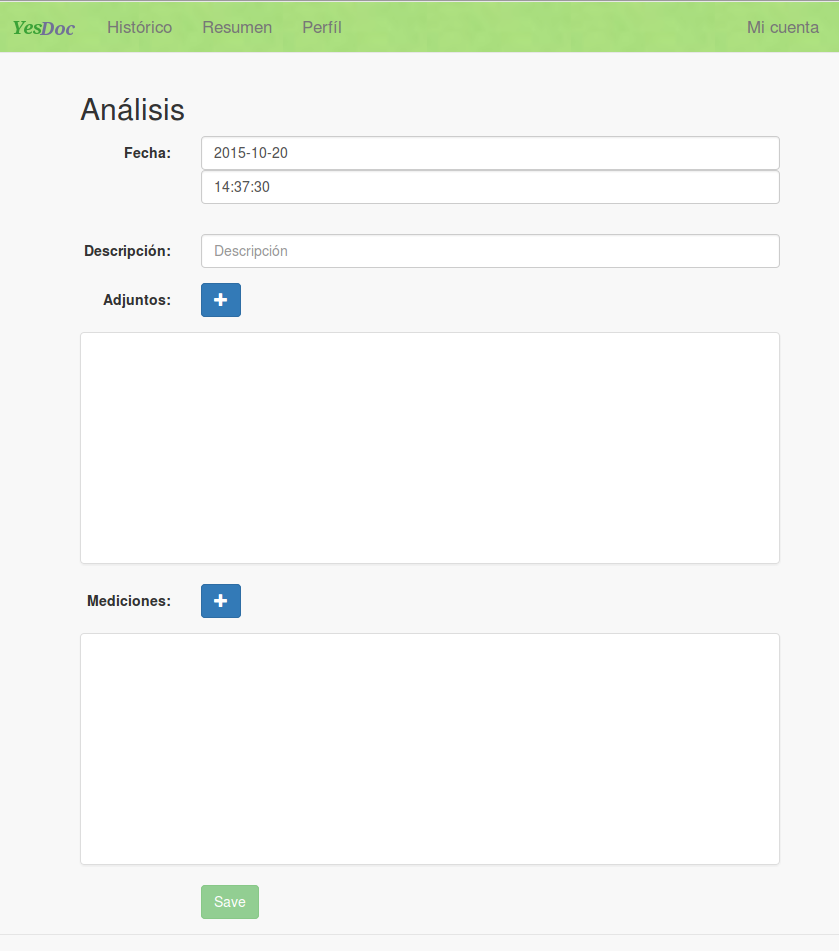
\includegraphics[width=0.5\textwidth]{img/5-crear_analisis}
        \caption{formulario para la creación de análisis}
		\label{5-crear_analisis}
    \end{figure}
    
    \begin{figure}[h]
        \centering
        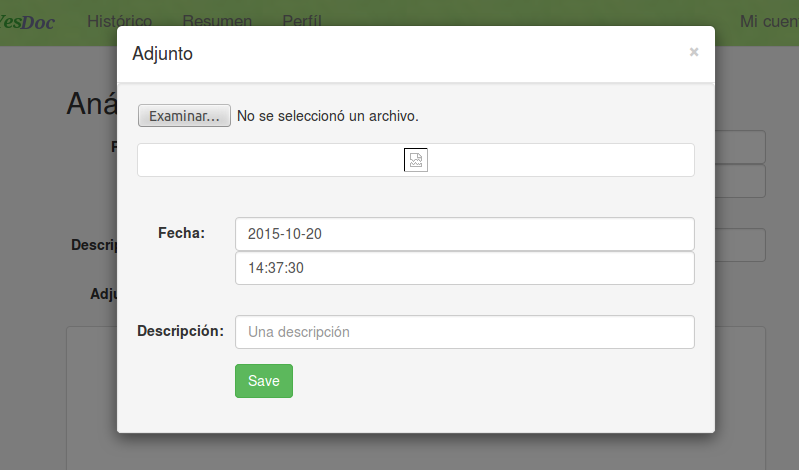
\includegraphics[width=0.5\textwidth]{img/5-cargar_img}
        \caption{formulario de carga de imágenes}
		\label{5-cargar_img}
    \end{figure}
    \begin{figure}[h]
        \centering
        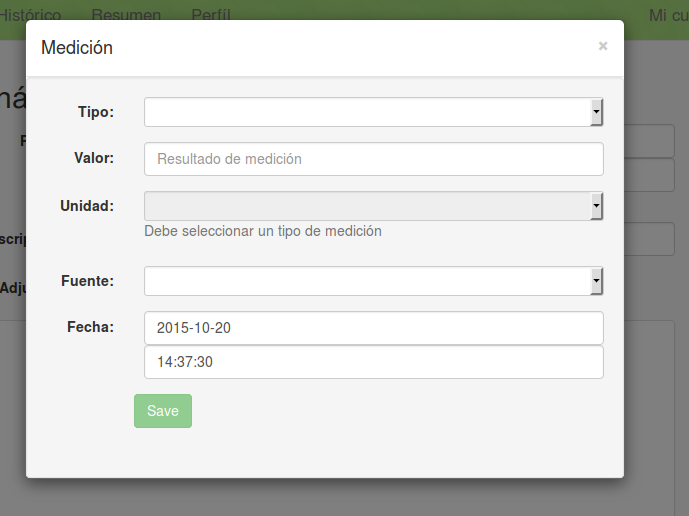
\includegraphics[width=0.5\textwidth]{img/5-cargar_medicion}
        \caption{formulario de carga de medición}
		\label{5-cargar_medicion}
    \end{figure}

    \begin{figure}[h]
        \centering
        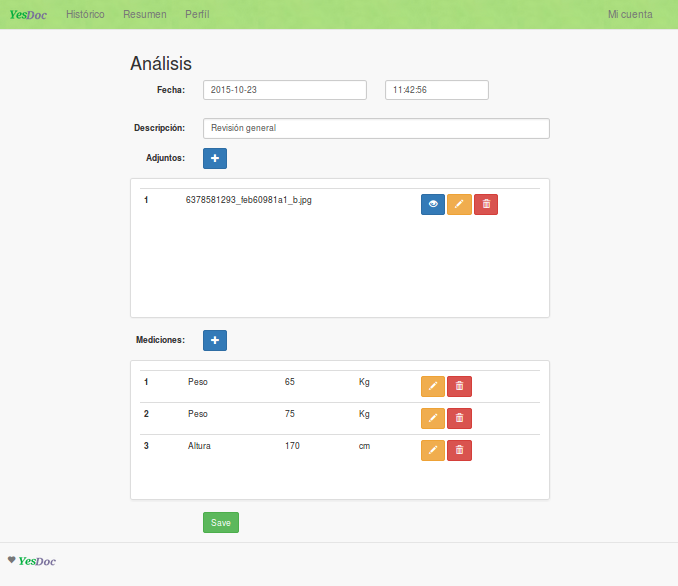
\includegraphics[width=0.5\textwidth]{img/5-mediciones_cargadas}
        \caption{Función de editar, borrar y visualizar}
		\label{5-mediciones_cargadas}
    \end{figure}


\clearpage

\subsection{Criterios de aceptación}

\begin{center}
\begin{longtable}{|p{0.7cm}|p{4cm}|p{4cm}|p{5cm}| }

	\hline 
		\rowcolor[gray]{0.9} 
		\multicolumn{4}{|c|}{\textbf{Criterio de aceptación}} \\
	\hline
    	\rowcolor[gray]{0.9} 
    	\multicolumn{1}{|c}{\textbf{Id}} & \multicolumn{1}{|c}{\textbf{Contexto}} &  \multicolumn{1}{|c}{\textbf{Evento}} & \multicolumn{1}{|c|}{\textbf{Resultado}} \\
    \hline
    	
1&En caso de que exista una persona sin mediciones & cuando este desee observar sus mediciones  & El sistema no mostrará nada \\ \hline
 
2& Cuando el usuario registrado ingresa dos mediciones del mismo tipo  & y luego quiera consultarlas & El sistema solo le mostrará la ultima medición, del mismo tipo, realizada\\ \hline

3& Cuando el usuario seleccione una medición & y luego quiera editarla & El sistema le permitira la correspondiente edición\\ \hline

4& Si el usuario existe y no está logeado & y quiera ingresar a ver sus mediciones. & El sistema no le permitirá ingresar\\ \hline

5& Si existe al menos un análisis cargado & al solicitar el servicio get del recurso AnalysisList & El sistema retorna una representación en cuyo cuerpo contiene una lista de análisis cargados en el sistema y el código de estado HTTP 200\\ \hline

6& Si existe un perfil cargado con el identificador indicado & l solicitar el servicio get del recurso AnalysisList & El sistema retorna una representación en cuyo cuerpo contiene los datos del análisis cargado en el sistema y el código de estado HTTP 201\\ \hline

7& Si no existe un análisis cargado con el identificador indicado & al solicitar el servicio get del recurso AnalysisView & El sistema retorna una respuesta con código de estado HTTP 404\\ \hline
  \end{longtable}
\end{center}


\subsection{Casos de prueba}

\subsubsection{Pruebas  de  integración  entre módulos del Sistema}


\begin{longtable}{|p{4cm}|p{4cm}|p{4cm}|p{3cm}|}
\hline
Actor  & Sistema& Resultado Esperado & Resultado obtenido \\ \hline

El usuario intenta ingresar al sistema & El sistema valida que el usuario con la contraseña ingresada exista 
& Se muestra un cartel de aviso de \textbf{usuario o contraseña invalido} 
& Ok, aunque el cartel podría ser mas vistoso 
\\ \hline



El usuario selecciona \textbf{nuevo perfil}, para
crear una cuenta en YesDoc 
& El sistema direcciona a la vista de creación de perfil
& Muestra formulario de creación de perfil.
&
\\ \hline



 El usuario completa todos los campos y presiona save.
 Ingresa:
\begin{itemize}
	\item \textbf{Nombre de usuario:} Franco
	\item \textbf{Apellido:} Canizo
	\item \textbf{Fecha de nacimiento: }2015-10-90
	\item \textbf{Género: }Masculino
	\item \textbf{Email: }franco@franco
	\item \textbf{pass:}Franco

\end{itemize}
& El sistema anula el botón \textbf{guardar }hasta tanto el usuario cargue todos los campos. una vez cargado todos los campos,al presionar save, redirecciona al menu
de logueo de usuario.
& El sistema informa que ha sido generado su usuario y lo direcciona al formulario de login.
& Ok, pero muestra ciertos mensajes de error al enviar el formulario \textbf{[Issue \#50]}
\\ \hline



El usuario ingresa 
	\textit{\begin{itemize}
		\item \textbf{Nombre de usuario:}Franco
		\item \textbf{Password: }Franco
	\end{itemize} }
&	El sistema valida usuario y contraseña,genera el token, direcciona a myProfileInformation y consulta a la API por la información personal \textbf{Figura \ref{5-login}}
& Se muestra la vista de perfil del usuario indicando sus datos personales
 \begin{itemize}
 		\item \textbf{Nombre de usuario:} Franco 
 		\item \textbf{Apellido: }Canizo 
 		\item \textbf{Fecha de nacimiento: }2015-10-90 
 		\item \textbf{Género: }Masculino
 	\end{itemize}
& Todo Ok, pero podrían aumentarse los colores y quitar espacios en blanco
\\ \hline


Presiona el boton \textit{\textbf{``Editar Perfil'' }}
& El sistema carga la vista \textbf{``profileinformation-edit.html''}, carga la vista correspondiente , valida que el usuario se encuentre logueado pasándole el token que se encuentra almacenado en las cookies. Solicita ala API los datos del perfil y del genero
para rellenar el formulario.
& Se muestra el formulario con los datos del perfil a editar.
& No carga los datos del usuario \textbf{[Issue \#47]}
\\ \hline



Cambia
\textit{
\begin{enumerate}
	\item \textbf{Nombre de usuario :} Franco Nicolás
\end{enumerate}}
&
& Muestra el cambio
& Ok
\\ \hline


Guarda los datos presionando en \textit{\textbf{``guardar''}} 
& El sistema se conecta con la API y guarda los datos a través del método PUT. Redirecciona al perfil de usuario y muestra los datos cambiados
&
Se muestra el perfil con los.
\textit{
\begin{itemize}
	\item \textbf{Nombre de usuario:} Franco Nicolas
	\item \textbf{Apellido:} Canizo
	\item \textbf{Fecha de Nacimiento: }2015-10-90
	\item \textbf{Género:} Masculino
	\item \textbf{Email: }franco@franco
\end{itemize}
}
& Guarda bien, pero al enviar el formulario muestra errores de validación \textbf{[Issue \#50]}
\\ \hline


El usuario presiona en \textbf{``Resumen'' } para ir a la sección donde se muestra una lista de cada medición con su último valor cargado.

& El sistema cambia la url por \textit{\textbf{``\#pro-fileMeasurements''}}, carga la vista correspondiente, valida que el usuario se encuentre logueado pasándole el token que se encuentra almacenado en las cookies y solicita al recurso de la API \textit{\textbf{``my/measurements/latest'' }}las últimas mediciones de cada tipo del usurario. \textbf{Figura \ref{5-perfil}}

& Se muestra una pantalla con dos botones uno para la carga de medición
\textit{\textbf{``Nueva Medición'' }}y otro para la carga de análisis \textit{\textbf{``Nuevo Análisis''}}. No se muestra más datos porque es un usuario nuevo sin información.\textbf{Figura \ref{5-perfil_mediciones}}
& OK
\\ \hline



Selecciona en \textbf{``Nueva análisis'' }
& El sistema direcciona a la url \textit{\textbf{"analy-sis/new"}}, carga la vista correspondiente, valida que el usuario se encuentre logueado pasándole el token que se encuentra almacenado en las cookies.

& Se muestra el formulario de carga de análisis \textbf{[Figura \ref{5-crear_analisis} ]}
& ok
\\ \hline



El usuario carga

\begin{itemize}
	\item \textbf{Fecha :}2015-09-30 16:10:59
	\item \textbf{Descripción: }revisión general
	\item Presionar en .\textbf{``Adjuntos''}

\end{itemize}

&
& El sistema muestra una ventana donde se puede cargar las imágenes con la medición y fecha.\textbf{ [Figura  \ref{5-cargar_img}]}
&ok

\\ \hline



Selecciona una imagen "jpg.o "png", de-ja la fecha igual. 
&
& Se muestra una imagen previa de la imagen. Se muestra la fecha En descripción se muestra el nombre de la imagen
& ok
\\ \hline
 
 

Presiona \textbf{\textit{``guardar''}}
&
& Muestra
\begin{itemize}
	\item Nombre de la descripción de la imagen.
	\item Iconos de visualizar,
	\item \textbf{Iconos de editar}
	\item \textbf{Iconos de borrar.}
\end{itemize}
& ok
\\ \hline





Seleccionar \textit{\textbf{``cargar Medición'' }}
& El sistema se conecta con la API para solicitar tipo y fuentes de mediciones
& El sistema muestra una ventana donde  se puede cargar las mediciones con los siguientes datos:
\textbf{\begin{itemize}
	\item ``Tipo'',
\item ``Valor''
\item ``Unidad''
\item ``Fuente''
\item ``Fecha''
\end{itemize}}
\textbf{[Figura \ref{5-cargar_medicion}]}
& ok
\\ \hline




Selecciona tipo:\textit{\textbf{ "peso"} }
	& El sistema se conecta con la API para
solicitar unidades relacionadas al tipo de medición peso con \textbf{id:``1'' }. \textbf{[Figura \ref{5-crear_medicion}]}
& Muestra las posibles unidades correspondientes al tipo peso
& ok
\\ \hline



Ingresa
\begin{itemize}
	\item \textbf{Tipo:} ``Peso''
	\item \textbf{valor: }``65''
	\item \textbf{Unidad:} ``kilogramo''
	\item \textbf{Fuente: }``manual''
	\item \textbf{Fecha: }``2015:-09-30 16:10:59''
	\item \textbf{ Guardar}
\end{itemize}
&
& Mantiene la misma venta abierta y muestra un mensaje de aviso de que la
medición fue cargada con éxito.\textit{ \textbf{"Bien hecho se cargo una medición''}}
& ok, si bien es útil que mantenga los datos para facilitar la nueva carga, sería conveniente acentuar el aviso de que la medición ya se cargo.
\\ \hline





Modificado el valor ingresado con anterioridad

\begin{itemize}
	\item \textbf{Tipo:} ``Peso''
	\item \textbf{valor: }``75''
	\item \textbf{Unidad:} ``kilogramo".
	\item \textbf{Fuente: }``manual"
	\item \textbf{Fecha: }2015:-10-10 16:10:59
	\item \textbf{ Guardar}
\end{itemize}
&
& Mantiene la misma venta abierta y muestra un mensaje de aviso de que la
medición fue cargada con éxito.\textbf{``Bien hecho se cargo una medición''}
& ok
\\ \hline




Selecciona



\begin{itemize}
	\item \textbf{Tipo:} ``altura'', modifica el valor ingresado con anterioridad
	por
	\item \textbf{valor: }``170''
	\item \textbf{Unidad:} ``centímetro".
	\item \textbf{Fuente: }``manual"
	\item \textbf{Fecha: }2015:-10-23 16:10:59
	\item \textbf{ Guardar}
\end{itemize}
&
&
Mantiene la misma venta abierta y muestra un mensaje de aviso de que
la medición fue cargada con éxito.\textit{\textbf{ ``Bien hecho se cargo una medición''}}
& ok
\\ \hline




Se selecciona el botón \textbf{"guardar"}
& El sistema consulta el perfil a la API para extraer el id el cual se usara para crear un análisis. Envía por POST a la API el análisis y realiza tres llamados mas a la API uno por cada medición cargada.
Mantiene la misma venta abierta y muestra un mensaje de aviso de que
la medición fue cargada con éxito. Almacena en la API el path y el storage\_location de la imagen.Luego direcciona la página a la url
\textit{\textbf{\#/profileMeasurements}}, valida que el token se encuentre activo, si no hay
errores solicita a la API las ultimas mediciones y muestra las mediciones

& En la vista de perfil de mediciones,Lista las últimas mediciones cargadas,
mostrando el peso cargado mas recientemente

\begin{itemize}
	\item Peso: 65 Kg Fecha 2015-10-2314:42:56 Manual
	\item Altura: 170 cm 2015-10-2314:42:56 Manual

\end{itemize}
& ok, habría que explicar que para ver todos sus pesos debería dirigirse a histórico

\\ \hline






Selecciona el icono de edición ubicado al lado de la medición \textit{Peso 65Kg}
& El sistema redirecciona \textbf{\#/measure-ments/103/edit}, verifica con la API que el token se encuentre activo, a partir del\textbf{ id} de la medición seleccionada para editar trae de la API el \textbf{tipo de medición, el valor, la unidad, la fuente y la fecha.}

& Se muestra un formulario con los datos de la medición precargadas
\begin{itemize}
	\item \textbf{Tipo:}Peso 
	\item \textbf{Valor: }65 
	\item \textbf{Unidad:} kilogramo
	\item \textbf{Fuente:}Manual 
	\item \textbf{Fecha:}2015-10-23 -14:42:56
\end{itemize}
&  ok
\\ \hline





Cambia la \textit{\textbf{fecha y la hora} por 2015-5-13- 4:42:56 }y guarda los cambios.
& El sistema guarda la medición, redirecciona\textbf{ \#/profileMeasurements }valida el token, y solicita las últimas mediciones a la API

& Muestra la interfaz con las últimas mediciones 
\begin{itemize}
	\item Peso: 75 Kg 2015-10-23 14:42:56 Manual 
	\item Altura: 170 cm 2015-10-23 14:42:56 Manual
\end{itemize}
& ok
\\ \hline





El usuario selecciona en \textit{\textbf{nueva medición}}
& El sistema redirecciona a \textbf{\#/measure-ments/new} valida contra la API que el Token se encuentra activo, luego trae los tipos de mediciones

& Muestra el formulario para cargar una medición con los siguientes valores 
\textbf{\begin{itemize}
	\item Tipo: 
	\item Valor:
	\item  Unidad: 
	\item Fuente: 
	\item Fecha:
\end{itemize}}
& ok
\\ \hline






El usuario selecciona en \textbf{``nueva medición''} 
\begin{itemize}
	\item \textbf{Tipo:}Peso
	\item \textbf{ Valor: }70
	\item\textbf{ Unidad:}-kilogramo
	\item \textbf{Fuente:}Manual
	\item \textbf{ Fecha:}2015-19-23 -14:42:56 
	\item \textbf{Guardar}
\end{itemize}

& El sistema redirecciona a \textbf{\#/profile-Measurementsvalida }contra la API que el Token se encuentra activo y luego trae las últimas mediciones

& Muestra la lista de últimas mediciones
\textbf{\begin{itemize}
	\item Peso: 75 Kg 2015-10-23 14:42:56 Manual
	\item Altura: 170 cm 2015-10-23 14:42:56 Ma-nual
\end{itemize}}
& ok
\\ \hline




Presionar en sección \textbf{``histórico''}
& El sistema redirecciona a\textbf{ \#/home }y se carga la vista correspondiente a  \textbf{  weight,} se verifica que el token este activo, se traen todas las medidas de tipo peso
& Se muestra una botonera con los tipos de mediciones , una gráfica y una tabla con las 3 medidas de tipo \textbf{Peso}
& ok, la botonera debería ser horizontal
\\ \hline




Presionar en sección \textbf{Altura }
& El sistema carga la vista correspondiente a height, se verifica que el token este activo, se traen todas las medidas de tipo peso
& Se muestra una botonera con los tipos de mediciones , una gráfica y una tabla con una medida \textbf{170 centímetros} de la altura.
& ok
\\ \hline





Presionar en sección \textit{\textbf{Análisis }} 
& El sistema carga la vista correspondiente a análisis, se verifica que el token este activo, se traen los análisis de la API
& Se muestra el análisis cargado con anterioridad mostrando la imagen, la descripción y la fecha seleccionada por el usuario.
& ok
\\ \hline






Selecciona el \textit{\textbf{Análisis}}
& El sistema carga la vista correspondiente a \textbf{ \#/home/analyses}, se verifica que el token este activo, trae los datos y los archivos del análisis de la API
& Se muestran las imágenes (en este caso sólo una) y una tabla con las mediciones de ese análisis.
& Falla en chrome, no muestra las imágenes
\\ \hline




Selecciona \textit{\textbf{Mi cuenta}}, luego \textit{\textbf{Cerrar Sesión}}
& El sistema direcciona \textbf{\#/logoof } y da de baja el token
& Se muestra la interface de login
& ok
\\ \hline


\end{longtable}







    \begin{figure}[h]
        \centering
        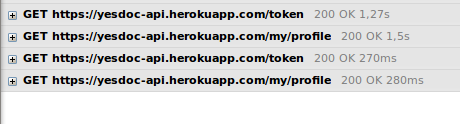
\includegraphics[width=0.5\textwidth]{img/5-login}
        \caption{Respuesta de la API al loguearse}
		\label{5-login}
    \end{figure}
    
        \begin{figure}[h]
        \centering
        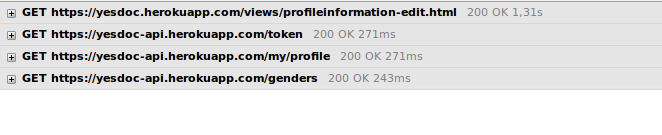
\includegraphics[width=0.5\textwidth]{img/5-perfil}
        \caption{Respuesta de la API al mostrar perfil}
		\label{5-perfil}
    \end{figure}
    
        \begin{figure}[h]
        \centering
        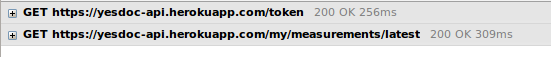
\includegraphics[width=0.5\textwidth]{img/5-resumen}
        \caption{Respuesta de la API al mostrar últimas mediciones}
		\label{5-resumen}
    \end{figure}
    
    \begin{figure}[h]
        \centering
        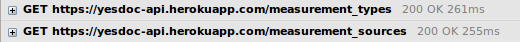
\includegraphics[width=0.5\textwidth]{img/5-crear_medicion}
        \caption{Respuesta de la API al crear nuevo análisis}
		\label{5-crear_medicion}
    \end{figure}
    
    
    
    
    \begin{figure}[h]
        \centering
        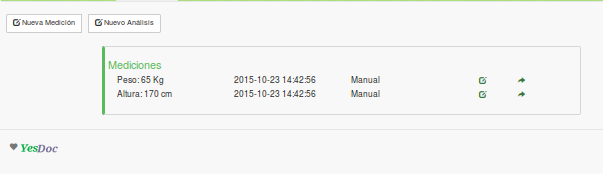
\includegraphics[width=0.5\textwidth]{img/5-perfil_mediciones}
        \caption{Perfil de mediciones}
		\label{5-perfil_mediciones}
    \end{figure}
    
    \begin{figure}[h]
        \centering
        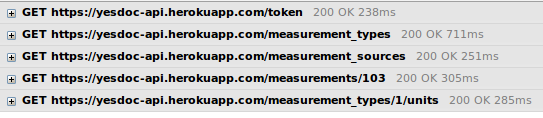
\includegraphics[width=0.5\textwidth]{img/5-editar_medicion}
        \caption{Respuesta de la API al editar mediciones}
		\label{5-editar_medicion}
    \end{figure}
    
    \begin{figure}[h]
        \centering
        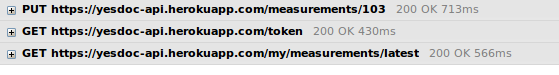
\includegraphics[width=0.5\textwidth]{img/5-fin_editar_medicion}
        \caption{Respuesta de la API al editar nuevo análisis}
		\label{5-fin_editar_medicion}
    \end{figure}
    
    \begin{figure}[h]
        \centering
        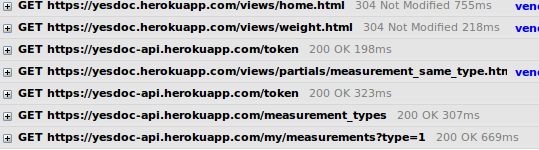
\includegraphics[width=0.5\textwidth]{img/5-mostrar_grafica}
        \caption{Respuesta de la API al mostrar gráficas}
		\label{5-mostrar_grafica}
    \end{figure}
    
    \begin{figure}[h]
        \centering
        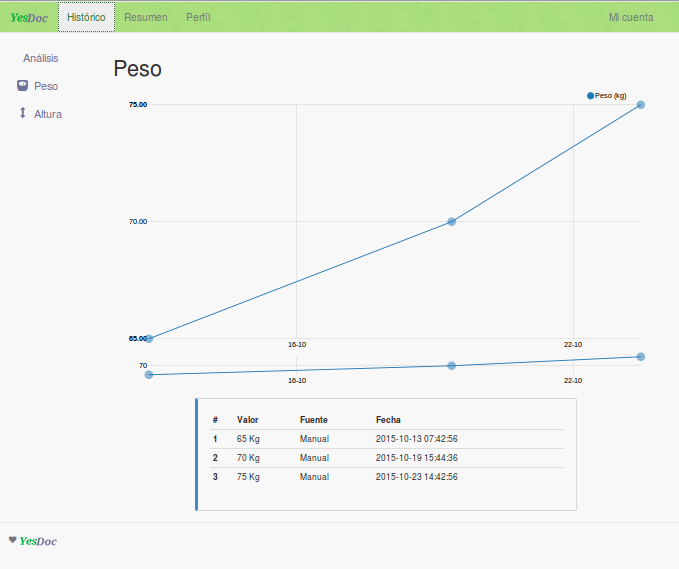
\includegraphics[width=0.5\textwidth]{img/5-grafica_medicion}
        \caption{Vista de gráfica y tablas de mediciones}
		\label{5-curva_medicion}
    \end{figure}
    
    \begin{figure}[h]
        \centering
        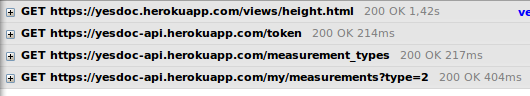
\includegraphics[width=0.5\textwidth]{img/5-grafica_altura}
        \caption{Respuesta de la API al mostrar la gráfica de altura}
		\label{5-grafica_altura}
    \end{figure}
    
    \begin{figure}[h]
        \centering
        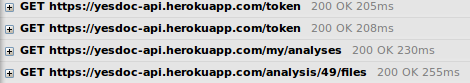
\includegraphics[width=0.5\textwidth]{img/5-mostrar_analisis}
        \caption{Respuesta de la API al mostrar los análisis}
		\label{5-mostrar_analisis}
    \end{figure}
    
    \begin{figure}[h]
        \centering
        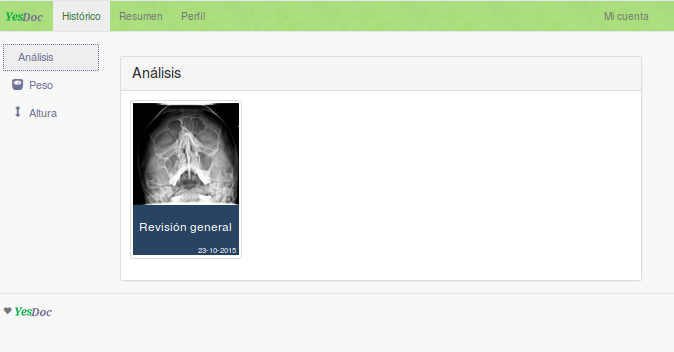
\includegraphics[width=0.5\textwidth]{img/5-mostrar_analisis_pag}
        \caption{Vista de la lista de análisis}
		\label{5-mostrar_analisis_pag}
    \end{figure}
    
    \begin{figure}[h]
        \centering
        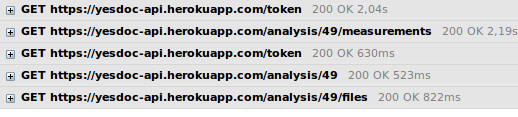
\includegraphics[width=0.5\textwidth]{img/5-analisis}
        \caption{Respuesta de la API al consultar los análisis}
		\label{5-analisis}
    \end{figure}
    
    \begin{figure}[h]
        \centering
        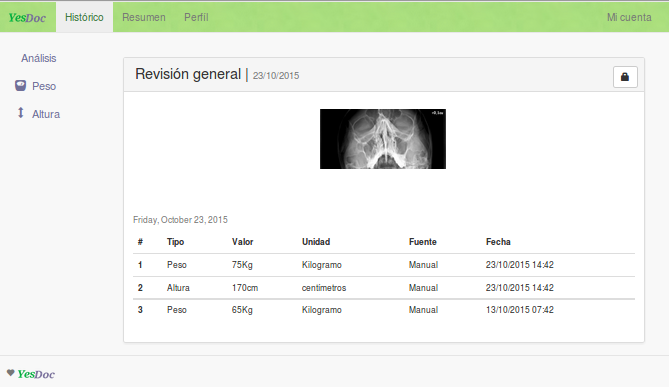
\includegraphics[width=0.5\textwidth]{img/5-contenido_analisis}
        \caption{Vista del contenido del análisis}
		\label{5-contenido_analisis}
    \end{figure}
    
    \begin{figure}[h]
        \centering
        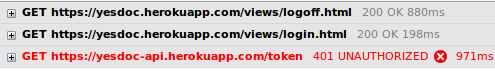
\includegraphics[width=0.5\textwidth]{img/5-logoff}
        \caption{Respuesta de la API al cerrar sesión}
		\label{5-logoff}
    \end{figure}
    



\clearpage



\subsubsection{Pruebas de carga}
Se va a simular el acceso a la página hosteada en heroku, de un lote de usuarios. Además en la gráfica \textbf{[Figura \ref{prueba_carga_50_us}]}se puede ver los tiempos de respuesta al ir incrementando la cantidad de usuarios.

\begin{center}
\begin{tabular}{|c|c|}
	\hline Cantidad de Usuario  &  Tiempo de espera\\ 
	\hline 20 usuarios &  155 ms \\ 
	\hline 30 usuarios  & 115 ms \\ 
	\hline 40 usuarios  & 100 ms \\ 
	\hline 50 usuarios  & 130 ms \\ 	
	\hline 
\end{tabular} 
\end{center}

    \begin{figure}[h]
    	\centering
    	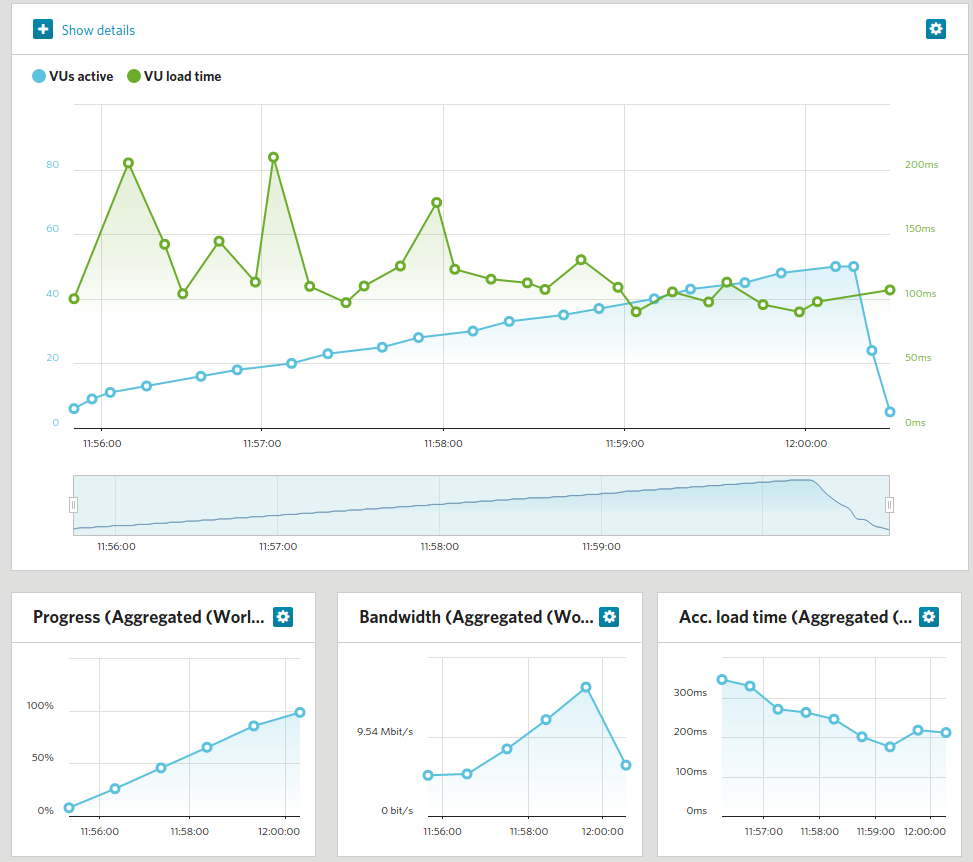
\includegraphics[width=0.5\textwidth]{img/prueba_carga_50_us}
    	\caption{Prueba de carga simulando 50 usuarios}
    	\label{prueba_carga_50_us}
    \end{figure}


\subsubsection{Pruebas de performance}
Google developers mide de 0 a 100 la velocidad de carga del sitio e indica, por orden de prioridad, qué mejorar, aportando información al respecto.
en nuestro caso nos recomienda disminuir el tamaño de las imágenes \textbf{[Figura \ref{prueba_velocidad_1}]}

\newpage

    \begin{figure}[h]
    	\centering
    	\includegraphics[width=0.5\textwidth]{img/prueba_velocidad_1}
    	\caption{Pruebas de velocidad en desktop}
    	\label{prueba_velocidad_1}
    \end{figure}

    \begin{figure}[h]
    	\centering
    	\includegraphics[width=0.5\textwidth]{img/prueba_velocidad_2}
    	\caption{Pruebas de velocidad pasadas}
    	\label{prueba_velocidad_2}
    \end{figure}

\newpage

\begin{longtable}{|p{1.0cm}|p{3cm}|p{3cm}|p{3.5cm}|p{2.5cm}|}
	\hline \hline
		\rowcolor[gray]{0.9} 
		\multicolumn{1}{|c}{ID} & \multicolumn{1}{|c|}{Descripción} & \multicolumn{1}{c|}{Precondiciones} & \multicolumn{1}{c|}{Pasos} &
		\multicolumn{1}{c|}{Resultado} \\
	\hline
	PC-1 & Se cargan 100 análisis a 5 perfiles  & Existen precargados instancias de Profile y Gender & Se generan instancias de Gender (Masculino y Femenino) y se generan 5 instancias de perfiles de usuarios diferentes, se hacen peticiones HTTP con método post al servicio \textbf{/analysis} & \textbf{Figura \ref{pc_a_1}} \\
	\hline
	PC-2 & Se obtienen 100 análisis de 5 perfiles & Existen precargados 100 análisis & Se cargan 100 análisis, se hace una petición http utilizando el método get al servicio \textbf{/analysis} & \textbf{Figura \ref{pc_a_2}}\\
		\hline

\end{longtable}

\begin{figure}[h]
    \centering
    \includegraphics[width=0.85\textwidth]{img/PC_analisis_1}
    \caption{Resultado prueba de carga de 100 análisis.}
	\label{pc_a_1}
\end{figure}

\begin{figure}[h]
    \centering
    \includegraphics[width=0.85\textwidth]{img/PC_analisis_2}
    \caption{Resultado prueba de obtención de 100 análisis.}
	\label{pc_a_2}
\end{figure}
\clearpage
\subsubsection{Pruebas de seguridad por niveles de usuarios}

\begin{longtable}{|p{1.0cm}|p{4cm}|p{4cm}|p{4cm}| }

	\hline
		\rowcolor[gray]{0.9} 
		\multicolumn{1}{|c}{Id test seguridad} & \multicolumn{1}{|c|}{Contexto} & \multicolumn{1}{|c|}{Evento} & \multicolumn{1}{|c|}{Resultado esperado} \\
	\hline
		ST-1 & Si el token utilizado en el header Authorization de la solicitud no corresponde a un usuario del sistema  & al solicitar el servicio put del recurso AnalysisView & El sistema retorna una respuesta con código de estado HTTP 401, UNAUTHORIZED\\
	\hline
		ST-2 & Si el token utilizado en el header Authorization de la solicitud corresponde a un usuario del sistema pero no al usuario al que pertenece el analysis & al solicitar el servicio put del recurso AnalysisView & El sistema retorna una respuesta con código de estado HTTP 403, FORBIDDEN\\
	\hline
		ST-3 & Si el token utilizado en el header Authorization de la solicitud corresponde a un usuario del sistema, el análisis con el identificador existe y el token pertenece al usuario al que pertenece el análisis & al solicitar el servicio put del recurso AnalysisView & El sistema retorna en el cuerpo de la respuesta los datos del análisis y el código de estado HTTP 200, UPDATED\\
	\hline
		ST-4 & Si el token utilizado en el header Authorization de la solicitud corresponde a un usuario del sistema, el análisis con el identificador existe y el token pertenece al usuario al que pertenece el análisis & al solicitar el servicio delete del recurso AnalysisView & El sistema retorna la respuesta con código de estado HTTP 204, DELETED\\
	\hline

\end{longtable}

\subsection{Pruebas ejecutadas}
	\begin{itemize}
		\item \textbf{¿Que fue bien?}
        	\begin{itemize}
				\item La carga de análisis, junto a las mediciones e imágenes funciona correctamente
				\item Listar los análisis y su contenido funcionan bien en Firefox.
				\item Se definió correctamente la gestión de análisis y el uso de autenticación para la gestión de análisis personales.
				\item Se armaron las vistas que permiten al usuario crear análisis y cargar mediciones e imágenes a los mismos.
			\end{itemize}
		\item \textbf{¿Que fue mal?}
		\begin{itemize}
			\item \textbf{Abierto} Las imágenes de los análisis no es posible verlo en el navegador Chrome.
			
		\end{itemize}
   		\item \textbf{¿Que se mejoró?}
        	\begin{itemize}
                \item \textbf{Cerrado} Los colores e imágenes de los botones.
                \item \textbf{Cerrado} Se permite hacer zoom en las gráficas.
                \item Se mejoró la captura de mediciones permitiendo que estas se engloben en el contexto de un análisis lo cual les da una razón de ser.
			\end{itemize}

   		\item \textbf{¿Que se puede mejorar?}
        	\begin{itemize}
		       \item \textbf{Abierto} La posición de la botonera en la sección histórico no es la correcta.
		       \item \textbf{Abierto}  El aviso de medición cargada debería ser mas nítido.
		       \item \textbf{Abierto} Al cargar un nuevo usuario y al modificarlo, el formulario muestra errores, esto produce desconcierto en el usuario.
		        \item Se debe mejorar en cuanto a los tiempos de trabajo del back end para brindar soluciones que puedan ser usadas a tiempo por el front end.
		        \item En cuanto a la gestión de análisis se podría definir que cuando el usuario cargue su primer medida del día, sin indicar un análisis específico, se cree automáticamente un análisis con descripción ``Análisis diario'' si es que éste aún no existe.
            \end{itemize}
        

	\end{itemize}
\clearpage


%%%%%%%%%%%%%%%%%%%%%%%%%%%%%%%%%%%%%%%%%%%%     FIN SPRINT 6   %%%%%%%%%%%%%%%%%%%%%%%%%%%%%%%%%%%%%%%%%%%%%%%%%%%%%%%5

\section{Sprint 7} % DROPBOX

\subsection{Planificación}


\textbf{Inicio:} Martes 1 de octubre del 2015

\textbf{Inicio:} Martes 17 de octubre del 2015



\subsection{Descripción}

En este sprint se busca brindarle al usuario la funcionalidad para poder gestionar imágenes. Son varios los casos en los que una persona concurre a una institución médico, realiza una serie de estudios como consecuencia de la consulta y obtiene resultados en forma de papel impreso o imágenes. Con la funcionalidad desarrollada en este sprint, el usuario puede tomar una imagen del documento o el archivo de la imagen tomada en el estudio, crear un análisis en yesdoc y adjuntar al análisis dichas imágenes. Podemos decir entonces que este análisis mantiene un respaldo digital de lo que es una consulta y de los documentos documentos resultantes de la misma, un análisis clínico, una imagen de radiografía y demás documentos médicos físicos. Para cumplir con esta funcionalidad el equipo tuvo que definir un medio de almacenamiento, para esto se eligió la nube. Existen muchos y variados medios de almacenamiento en la nube como son Dropbox, Drive, Mega, entre otros. Teniendo en cuenta esta situación, el equipo tuvo que definir una forma de conectarse con los mismos adaptando la comunicación de acuerdo a cada una en particular y reduciendo el impacto frente al cambio siempre teniendo en cuenta la alta cohesión y el bajo acoplamiento.
	
	
	Este sprint le permite al usuario:
	\begin{itemize}
		\item Elegir el medio de almacenamiento en la nube de preferencia y, en caso de que no cuente con uno, utilizar el que YesDoc ofrece por defecto.
		\item Brindar un flujo de autorización, por parte del usuario para que YesDoc use el almacenamiento seleccionado, integrado en el sistema y intuitivo.
		\item Cargar, descargar y eliminar imágenes en un análisis.
		\item Listar las imágenes de un análisis.
		\item Cambiar el medio de almacenamiento seleccionado cuando lo desee. % consultar si está implementado			
	\end{itemize}
	  


\subsection{Sprint backlog}


{\scriptsize
	\begin{center} %sidewaystable
		\centering
		%\begin{adjustbox}{max width=\textheight}
		\resizebox{\textwidth}{!}{
			\begin{tabular}{|l|l|l|p{6cm}|l|l|}
				\hline
				\textbf{Area a cargo} &
				\textbf{Responsable} &  
             	\textbf{Revisor} &       
				\textbf{Tarea} &
				\textbf{US} &
				\textbf{tiempo dedicado}\\ 
				\hline
				Back-end& Franco Canizo & Michael Manganiello & Se define la estructura para la gestión de archivos & US-\ref{resumenInfo} \& US-\ref{infoSalud} & 4hs \\ 
				\hline
				Back-end& Franco Canizo& Michael Manganiello & Se crea el adaptador para la gestión de archivos en dropbox , se crea el recurso para la carga y descarga de archivos de análisis. & US-\ref{resumenInfo} \& US-\ref{infoSalud} & 24hs \\ 
				\hline
				Back-end& Michael Manganiello & todos& Se añaden las clases del dominio y funcionalidades para el manejo de análisis, archivos asociados, y la gestión de credenciales a diferentes servicios de almacenamiento personales del usuario & US-\ref{resumenInfo} \& US-\ref{infoSalud} & 6hs \\ 
				\hline
				Back-end& Michael Manganiello &Franco Canizo & Creación de la migración para los nuevos modelos & US-\ref{resumenInfo} \& US-\ref{infoSalud} & 2hs \\ 
				\hline
				Back-end& Michael Manganiello &Franco Canizo & Creación de fields y parsers para las representaciones de los nuevos recursos & US-\ref{resumenInfo} \& US-\ref{infoSalud} & 2hs\\ \hline
				Back-end& Michael Manganiello & Franco Canizo & Correcciones generales de integración, claves de la aplicación en Dropbox, devolución y eliminación de archivos & US-\ref{resumenInfo} \& US-\ref{infoSalud} & 16hs\\ 
				\hline
			\end{tabular}
		}
		%\end{adjustbox}
	\end{center}
}

\subsection{User Stories relacionados}
La \textbf{Tabla \ref{US-Sprint6} } indicará las características de cada user story para guiarnos en el desarrollo del sprint.

\begin{table}[h]
    \label{US-Sprint7}
	%\resizebox{\textwidth}{!}{
    \centering
	\begin{tabular}{|l|p{9cm}|}
	\hline
        \multicolumn{1}{|c|}{\textbf{ID}} &
        \multicolumn{1}{|c|}{\textbf{Enunciado de la historia}} \\          
    \hline
        \textbf{US-1 } & Como paciente, quiero  añadir información de mi perfil de salud o mediciones regulares para que el médico cuente con más y mejor información al momento de realizar el diagnóstico. \\
    \hline
        \textbf{US-2 } & Como paciente, quiero añadir al sistema los estudios realizados para evitar posibles perdidas.\\
     \hline
        \textbf{US-16 } & Como paciente, quiero acceder a mis documentos desde cualquier lugar para hacer uso de ellos cuando los necesite.\\
     \hline   
     
    \end{tabular}
%     }
\end{table}

\subsection{Modelo funcional} 
Se describirán las funciones usando como marco de apoyo el sprint Backlog, además se armará el diagrama de casos de uso del presente Sprint \textbf{[Figura \ref{6-cu_file_upload}]} que irá creciendo  medida se vaya avanzando en el proyecto.

    \begin{figure}[h]
        \centering
        \includegraphics[width=0.5\textwidth]{img/cu_file_upload}
        \caption{CU-Gestión de archivos}
		\label{6-cu_file_upload}
    \end{figure}
    
\newpage

\subsection{Modelo de datos}
El Diagrama propio de este sprint se puede ver en la \textbf{Figura\ref{6-clases_file_upload}}, allí se indican exactamente las clases que se usarán en este sprint y que serán detalladas con detenimiento en el presente documento. Se recuerda que se ha realizado un Diagrama de clases específico para este sprint y puede variar en futuras iteraciones.
% Se fue a la mierda esta imágen
    \begin{figure}[h]
        \centering
        \includegraphics[width=0.5\textwidth]{img/dc_file_upload}
        \caption{Clases para la gestión de archivos.}
		\label{6-clases_file_upload}
    \end{figure}


\subsection{Diseño} 

\subsubsection{Estructura conexión con diferentes medios de almacenamiento}
	Se define el paquete ``adapters'' en el cual se define una fábrica encargada de la creación del adaptador específico para la conexión y gestión de archivos con el medio de almacenamiento específico. Para la situación actual del sistema se definen dos adaptadores específicos, uno para el almacenamiento por defecto en la cuenta de YesDoc y otro para el almacenamiento de archivos en Dropbox. La \textbf{Figura \ref{6-dcd_file_upload}} muestra el diagrama de clases de diseño específico.

	\begin{figure}[h]
        \centering
        \includegraphics[width=0.9\textwidth]{img/dcd_file_upload}
        \caption{DCD-Carga de archivos}
		\label{6-dcd_file_upload}
    \end{figure}
   
\newpage

	En este diseño se aplicaron los patrones:
		\begin{itemize}			
			\item Alta cohesión.
			\item Bajo acoplamiento.
			\item Singleton
			\item Factoría
			\item Adaptador
		\end{itemize}

\subsubsection{Modelos para la gestión de archivos}

Se crean las clases del modelo lógico que definimos en la \textbf{Figura\ref{6-clases_file_upload}}, de cada una de estas se definen los atributos siguiendo la documentación de SQLAlchemy, ORM utilizado para mapeo de las entidades de la API, sus relaciones y funcionalidades. 

El modelo \textbf{StorageCredential} guarda el token que recibe la API luego de que el usuario autorice a la aplicación a usar su almacenamiento en dropbox para gestionar archivos. Cada StorageCredential mantiene una relación con User y StorageCredential.

El modelo \textbf{StorageLocation} mantiene un identificador y datos generales del medio de almacenamiento de preferencia del usuario a partir de los ofrecidos por la API.

El modelo \textbf{AnalysisFile} mantiene datos relacionados con la gestión del archivo como la ruta, nombre, fecha de carga y está relacionado con el modelo Analysis y StorageLocation lo que nos permite asignar varios archivos a un análisis, archivos que pueden estar almacenados en distintos medios de almacenamiento en la nube.

\subsubsection{Creación de la migración para los nuevos modelos}

Una vez definidas las clases se obtiene a partir de migrate un script sql con la nueva versión de la base de datos, script que utilizamos para actualizar las tablas de la base de datos para incorporar las nuevas a partir de los modelos previamente definidos. Esto es posible gracias al uso de las extensiones \textbf{flask-migrate} para las migraciones de la base de datos y \textbf{flask-script} para la ejecución de comandos externos.

\subsubsection{Definición de Recursos}

Para que el cliente se comunique con los modelos que hemos definido la API define recursos encargadas de manejar estos modelos:

El recurso \textbf{AnalysisAnalysisFileList} permite la obtención de los archivos asociados a un análisis específico. El usuario debe estar autenticado. El servicio se brinda a través del método GET.

\textbf{AnalysisFileDownload} permite la descarga de un archivo específico desde el medio de almacenamiento en la nube. Requiere autenticación. El servicio se brinda a través del método GET.

\textbf{AnalysisFileThumbnail} permite obtener la vista previa de un archivo específico. Requiere autenticación. El servicio se brinda a través del método GET.

\textbf{AnalysisFileView} permite obtener, a través del servicio GET, datos cargados en el modelo AnalysisFile, por medio de PUT se  puede modificar los datos almacenados de un archivo y DELETE para eliminar los datos y el archivo correspondiente en la nube. Todos estos servicios mencionados requieren previa autenticación.

El método auxiliar delete\_file en el archivo \textbf{analysisFile} en el directorio ``persistence'' elimina un archivo del medio de almacenamiento en la nube.

\textbf{AnalysisFileList} brinda servicio GET para obtener todas las instancias de AnalysisFile correspondientes a los archivos cargados a YesDoc y, a través del servicio POST, cargar un nuevo AnalysisFile y el archivo al medio de almacenamiento de preferencia para el usuario. El servicio POST requiere autenticación.

\textbf{StorageCredentialView} brinda los servicios GET para obtener una instancia específica de credencial y PUT para actualizar una instancia específica de StorageCredential.

\textbf{StorageCredentialList} brinda los servicios GET para obtener las credenciales de almacenamiento cargadas y POST para cargar una nueva credencial de almacenamiento.

\textbf{StorageLocationView} brinda los servicios GET para obtener una instancia específica de ubicación de almacenamiento y PUT para actualizar una instancia específica de ubicación de almacenamiento.	

\textbf{StorageLocationList} brinda los servicios GET para obtener todas las ubicaciones de almacenamiento cargadas y POST para cargar una nueva ubicación de almacenamiento.

\textbf{MyStorageCredentialList} por medio del servicio GET retorna todas las instancias existentes de credencial de almacenamiento, asociadas al usuario autenticado. A través del servicio POST crea una nueva instancia de credencial de almacenamiento asociada al usuario autenticado, y la retorna.

Se añade al recurso \textbf{AnalysisView} el servicio DELETE para eliminar todas las imágenes asociadas a un análisis específico. Elimina también el análisis. Requiere que el usuario esté autenticado.

\subsubsection{Identificadores(URI)}
Para acceder a estos recurso el equipo pone a disposición del cliente los siguientes identificadores:

\begin{itemize}
	\item\textbf{/analysis/<int:analysis\_id>/files}
	\item\textbf{/analysis/<int:analysis\_id>}
	\item\textbf{/analysis\_files/<int:id>/download}
	\item\textbf{/analysis\_files/<int:analysis\_file\_id>/thumbnail}
	\item\textbf{/analysis\_files/<int:id>}
	\item\textbf{/analysis\_files}
	\item\textbf{/storage\_credentials/<int:id>}
	\item\textbf{/storage\_credentials}
	\item\textbf{/storage\_locations/<int:id>}
	\item\textbf{/storage\_locations}
	\item\textbf{/my/storage\_credentials}
\end{itemize}

\subsubsection{Representaciones}
Finalmente se arman las representaciones que el cliente debe tener en cuenta al momento de enviar y recibir datos. Las definiciones bajo el directorio ``parsers'' determinan la representación para las solicitudes HTTP del cliente al servidor mientras que las definidas bajo el directorio ``fields'' definen la representación para las respuestas del servidor al cliente.





\subsection {Salidas del Sistema - Incrementos}
\textbf{Carga de una credencial de almacenamiento}

Para la carga debemos utilizar el recurso que la API presenta con el identificador único URL \textbf{\/storage\_credentials}. Suponemos que previamente el usuario de prueba ha autorizado a nuestra aplicación a que utilice espacio del almacenamiento de su cuenta de dropbox y por lo tanto contamos con el token: ``Jl0\_uroqYBoAAAAAAAA
F6KUxPAlgAMTqFf9ES2S0zZl\_27V5QAmEn5V58IUxcck1''. Suponemos que ha sido cargado en API un usuario con id 1 y un storage location con id 2. Teniendo en cuenta la representación definida para la solicitud al recurso y que debemos usar el método POST para cargar la credencial, ejecutamos la siguiente linea CURL:

\begin{verbatim}
curl -i http://localhost:5000/storage_credentials -H "Content-Type: 
application/json" -X POST -d '{"token":"Jl0_uroqYBoAAAAAAAAF6KUxPAl
gAMTqFf9ES2S0zZl_27V5QAmEn5V58IUxcck1", "owner_id":"1", 
"storage_location_id":"1"}'
\end{verbatim}

La API nos responde con la siguiente respuesta:

\begin{lstlisting}[language=json]
HTTP/1.0 201 CREATED
Content-Type: application/json
Content-Length: 812
Server: Werkzeug/0.10.4 Python/2.7.6
Date: Tue, 20 Oct 2015 19:10:33 GMT

{
    "resource": {
        "id": 2, 
        "owner": {
            "email": "fncanizo@gmail.com", 
            "id": 1, 
            "profile": {
                "birthday": "1990-06-20", 
                "first_name": "Franco", 
                "gender": {
                    "description": "male gender", 
                    "id": 1, 
                    "name": "male"
                }, 
                "id": 1, 
                "last_name": "Canizo"
            }, 
            "username": "coco19"
        }, 
        "storage_location": {
            "description": "yesdoc file manager", 
            "id": 2, 
            "name": "YesDoc", 
            "website": "http://yesdoc.herokuapp.com"
        }, 
        "token": "Jl0_uroqYBoAAAAAAAAF6KUxPAlgAMTqFf9ES2S0zZl_27V5QAmEn5V58IUxcck1"
    }
}
\end{lstlisting}



\clearpage
\subsection{Criterios de aceptación}
\textbf{Ejemplo - esto se debe modificar}


\begin{center}
\begin{longtable}{|p{0.7cm}|p{4cm}|p{4cm}|p{5cm}| }

	\hline 
		\rowcolor[gray]{0.9} 
		\multicolumn{4}{|c|}{\textbf{Criterio de aceptación}} \\
	\hline
    	\rowcolor[gray]{0.9} 
    	\multicolumn{1}{|c}{\textbf{Id}} & \multicolumn{1}{|c}{\textbf{Contexto}} &  \multicolumn{1}{|c}{\textbf{Evento}} & \multicolumn{1}{|c|}{\textbf{Resultado}} \\
    \hline
    	
1&Usuario autenticado, análisis inexistente & cuando el usuario intenta cargar una imágene en el análisis & El sistema responderá con un código de estado 404 NOT FOUND\\ \hline
 
2& Usuario autenticado, análisis existente   & al cargarlo & El sistema responderá con el código de estado 201 CREATED y los metadatos del archivo en el cuerpo de la respuesta\\ \hline

3& Usuario autenticado, archivo existente & al solicitar el obtener el archivo & el sistema responderá con el código 200 y devolverá los datos del archivo\\ \hline

4& Usuario autenticado, archivo existente, descripción distinta de la descripción de la imagen & cuando solicite actualizar el archivo & El sistema responderá con código 200 y devolverá datos actualizados del archivo\\ \hline

5& Usuario autenticado, archivo existente & cuando solicite eliminar el archivo & El sistema responde con el código de estado HTTP 204 y el usuario puede verificar que el archivo ya no se encuentra en su medio de almacenamiento.\\ \hline

  \end{longtable}
\end{center}


\subsection{Casos de prueba}

\subsubsection{Pruebas  de  integración  entre módulos del Sistema}

Se realizarán pruebas para verificar que el desarrollo de carga de archivos se integra bien a los desarrollos de gestión de análisis y de mediciones. Suponemos usuario logeado.

\begin{longtable}{|p{4cm}|p{4cm}|p{4cm}|p{3cm}|}
\hline
Actor  & Sistema& Resultado Esperado & Resultado obtenido \\ \hline

Selecciona en \textbf{``Nuevo análisis'' }
& El sistema redirecciona a la url \textit{\textbf{``analysis/new''}}, carga la vista correspondiente, valida que el usuario se encuentre logueado pasándole el token que se encuentra almacenado en las cookies.

& Se muestra el formulario de carga de análisis \textbf{[Figura \ref{5-crear_analisis} ]}
& ok
\\ \hline



El usuario carga

\begin{itemize}
	\item \textbf{Fecha :}2015-09-30 16:10:59
	\item \textbf{Descripción: }revisión general
	\item Presionar en .\textbf{``Adjuntos''}

\end{itemize}

&
& El sistema muestra una ventana donde se puede cargar las imágenes con la medición y fecha.\textbf{ [Figura  \ref{5-cargar_img}]}
&ok

\\ \hline



Selecciona una imagen "jpg.o "png", de-ja la fecha igual. 
&
& Se muestra una imagen previa de la imagen. Se muestra la fecha En descripción se muestra el nombre de la imagen
& ok
\\ \hline
 
 

Presiona \textbf{\textit{``guardar''}}
&
& Muestra
\begin{itemize}
	\item Nombre de la descripción de la imagen.
	\item Iconos de visualizar,
	\item \textbf{Iconos de editar}
	\item \textbf{Iconos de borrar.}
\end{itemize}
& ok
\\ \hline





Seleccionar \textit{\textbf{``cargar Medición'' }}
& El sistema se conecta con la API para solicitar tipo y fuentes de mediciones
& El sistema muestra una ventana donde  se puede cargar las mediciones con los siguientes datos:
\textbf{\begin{itemize}
	\item ``Tipo'',
\item ``Valor''
\item ``Unidad''
\item ``Fuente''
\item ``Fecha''
\end{itemize}}
\textbf{[Figura \ref{5-cargar_medicion}]}
& ok
\\ \hline




Selecciona tipo:\textit{\textbf{ "peso"} }
	& El sistema se conecta con la API para
solicitar unidades relacionadas al tipo de medición peso con \textbf{id:``1'' }. \textbf{[Figura \ref{5-crear_medicion}]}
& Muestra las posibles unidades correspondientes al tipo peso
& ok
\\ \hline



Ingresa
\begin{itemize}
	\item \textbf{Tipo:} ``Peso''
	\item \textbf{valor: }``65''
	\item \textbf{Unidad:} ``kilogramo''
	\item \textbf{Fuente: }``manual''
	\item \textbf{Fecha: }``2015:-09-30 16:10:59''
	\item \textbf{ Guardar}
\end{itemize}
&
& Mantiene la misma venta abierta y muestra un mensaje de aviso de que la
medición fue cargada con éxito.\textit{ \textbf{"Bien hecho se cargo una medición''}}
& ok, si bien es útil que mantenga los datos para facilitar la nueva carga, sería conveniente acentuar el aviso de que la medición ya se cargo.
\\ \hline





Modificado el valor ingresado con anterioridad

\begin{itemize}
	\item \textbf{Tipo:} ``Peso''
	\item \textbf{valor: }``75''
	\item \textbf{Unidad:} ``kilogramo".
	\item \textbf{Fuente: }``manual"
	\item \textbf{Fecha: }2015:-10-10 16:10:59
	\item \textbf{ Guardar}
\end{itemize}
&
& Mantiene la misma venta abierta y muestra un mensaje de aviso de que la
medición fue cargada con éxito.\textbf{``Bien hecho se cargo una medición''}
& ok
\\ \hline




Selecciona



\begin{itemize}
	\item \textbf{Tipo:} ``altura'', modifica el va-lor ingresado con anterioridad
	por
	\item \textbf{valor: }``170''
	\item \textbf{Unidad:} ``centimetro".
	\item \textbf{Fuente: }``manual"
	\item \textbf{Fecha: }2015:-10-23 16:10:59
	\item \textbf{ Guardar}
\end{itemize}
&
&
Mantiene la misma venta abierta y muestra un mensaje de aviso de que
la medición fue cargada con éxito.\textit{\textbf{ ``Bien hecho se cargo una medición''}}
& ok
\\ \hline




Se selecciona el botón \textbf{"guardar"}
& El sistema consulta el perfil a la API para extraer el id el cual se usara para crear un análisis. Envia por POST a la API el análisis y realiza tres llamados mas a la API uno por cada medicióncargada.
Mantiene la misma venta abierta y muestra un mensaje de aviso de que
la medición fue cargada con éxito. Almacena en la API el path y el storage\_location de la imagen.Luego redirecciona la paágina a la url
\textit{\textbf{\#/profileMeasurements}}, valida que el token se encuentre activo, si no hay
errores solicta a la API las ultimas mediciones y muestra las mediciones

& En la vista de perfil de mediciones,Lista las últimas mediciones cargadas,
mostrando el peso cargado mas recientemente

\begin{itemize}
	\item Peso: 65 Kg Fecha 2015-10-2314:42:56 Manual
	\item Altura: 170 cm 2015-10-2314:42:56 Manual

\end{itemize}
& ok, habría que explicar que para ver todos sus pesos debería dirigirse a histórico

\\ \hline






Selecciona el icono de edición ubicado al lado de la medición \textit{Peso 65Kg}
& El sistema redirecciona \textbf{\#/measure-ments/103/edit}, verifica con la API que el token se encuentre activo, a partir del\textbf{ id} de la medición seleccionada para editar trae de la API el \textbf{tipo de medición, el valor, la unidad, la fuente y la fecha.}

& Se muestra un formulario con los datos de la medición precargadas
\begin{itemize}
	\item \textbf{Tipo:}Peso 
	\item \textbf{Valor: }65 
	\item \textbf{Unidad:} kilogramo
	\item \textbf{Fuente:}Manual 
	\item \textbf{Fecha:}2015-10-23 -14:42:56
\end{itemize}
&  ok
\\ \hline





Cambia la \textit{\textbf{fecha y la hora} por 2015-5-13- 4:42:56 }y guarda los cambios.
& El sistema guarda la medición, redirecciona\textbf{ \#/profileMeasurements }valida el token, y solicita las últimas mediciones a la API

& Muestra la interfaz con las últimas mediciones 
\begin{itemize}
	\item Peso: 75 Kg 2015-10-23 14:42:56 Manual 
	\item Altura: 170 cm 2015-10-23 14:42:56 Manual
\end{itemize}
& ok
\\ \hline





El usuario selecciona en \textit{\textbf{nueva medición}}
& El sistema redirecciona a \textbf{\#/measure-ments/new} valida contra la API que el Token se encuentra activo, luego traelos tipos de mediciones

& Muestra el formulario para cargar una medición con los siguientes valores 
\textbf{\begin{itemize}
	\item Tipo: 
	\item Valor:
	\item  Unidad: 
	\item Fuente: 
	\item Fecha:
\end{itemize}}
& ok
\\ \hline






El usuario selecciona en \textbf{``nueva medición''} 
\begin{itemize}
	\item \textbf{Tipo:}Peso
	\item \textbf{ Valor: }70
	\item\textbf{ Unidad:}-kilogramo
	\item \textbf{Fuente:}Manual
	\item \textbf{ Fecha:}2015-19-23 -14:42:56 
	\item \textbf{Guardar}
\end{itemize}

& El sistema redirecciona a \textbf{\#/profile-Measurementsvalida }contra la API que el Token se encuentra activo y luego trae las últimas mediciones

& Muestra la lista de últimas mediciones
\textbf{\begin{itemize}
	\item Peso: 75 Kg 2015-10-23 14:42:56 Manual
	\item Altura: 170 cm 2015-10-23 14:42:56 Ma-nual
\end{itemize}}
& ok
\\ \hline

Presionar en sección \textbf{``histórico''}
& El sistema redirecciona a\textbf{ \#/home }y se carga la vista correspondiente a  \textbf{  weight,} se verifica que el token este activo, setraen todas las medidas de tipo peso
& Se muestra una botonera con los tipos de mediciones , una gráfica y una tabla con las 3 medidas de tipo \textbf{Peso}
& ok, la botonera debería ser horizontal
\\ \hline

Presionar en sección \textbf{Altura }
& El sistema carga la vista correspondiente a height, se verifica que el token este activo, se traen todas las medidas de tipo peso
& Se muestra una botonera con los tipos de mediciones , una gráfica y una tabla con una medida \textbf{170 centímetros} de la altura.
& ok
\\ \hline

Presionar en sección \textit{\textbf{Análisis }} 
& El sistema carga la vista correspondiente a análisis, se verifica que el token este activo, se traen los análisis de la API
& Se muestra el análisis cargado con anterioridad mostrando la imagen, la descripción y la fecha seleccionada por el usuario.
& ok
\\ \hline

Selecciona el \textit{\textbf{Análisis}}
& El sistema carga la vista correspondiente a \textbf{ \#/home/analyses}, se verifica que el token este activo, trae los datos y los archivos del análisis de la API
& Se muestran las imágenes (en este caso sólo una) y una tabla con las mediciones de ese análisis.
& Falla en chrome, no muestra las imágenes
\\ \hline

Selecciona \textit{\textbf{Mi cuenta}}, luego \textit{\textbf{Cerrar Sesiónn}}
& El sistema direcciona \textbf{\#/logoof }y da debaja el token
& Se muestra la interface de login
& ok
\\ \hline

\end{longtable}
\clearpage
\subsubsection{Pruebas de carga}

Se prueba la carga de credenciales, no se prueba la carga de archivos por motivos de capacidad de almacenamiento.

\begin{longtable}{|p{1.0cm}|p{3cm}|p{3cm}|p{3.5cm}|p{2.5cm}|}
	\hline \hline
		\rowcolor[gray]{0.9} 
		\multicolumn{1}{|c|}{ID} & \multicolumn{1}{|c|}{Descripción} & \multicolumn{1}{c|}{Precondiciones} & \multicolumn{1}{c|}{Pasos} &
		\multicolumn{1}{c|}{Resultado} \\
	\hline
	PC-1 & Se cargan 50 credenciales a 5 usuarios diferentes  & Existen precargados instancias de User y StorageLocation y  & Se generan instancias de StorageLocation (YesDoc, Dropbox, Drive) y se generan 5 instancias de User diferentes, se hacen peticiones HTTP con método post al servicio \textbf{/storage\_credentials} & Latencias de respuesta baja %armarlo en jmeter 
	\\ \hline
	
\end{longtable}

\clearpage
\subsubsection{Pruebas de seguridad por niveles de usuarios}

\begin{longtable}{|p{1.0cm}|p{4cm}|p{4cm}|p{4cm}| }

	\hline
		\rowcolor[gray]{0.9} 
		\multicolumn{1}{|c}{Id test seguridad} & \multicolumn{1}{|c|}{Contexto} & \multicolumn{1}{|c|}{Evento} & \multicolumn{1}{|c|}{Resultado esperado} \\
	\hline
		ST-1 & Si el token utilizado en el header Authorization de la solicitud corresponde a un usuario del sistema, este tiene un análisis creado con imágenes asociadas al mismo  & al solicitar el servicio get por medio del identificador /analysis/<int:analysi-s\_id>/files & El sistema devuelve la respuesta con código de estado HTTP 200 OK y la lista de imágenes asociadas al análisis\\
	\hline
		ST-2 & Si el token utilizado en el header Authorization de la solicitud corresponde a un usuario del sistema pero no al usuario al que pertenece el analysis & al solicitar el servicio put del recurso AnalysisView & El sistema retorna una respuesta con código de estado HTTP 403, FORBIDDEN\\
	\hline
		ST-3 & Si el token utilizado en el header Authorization de la solicitud corresponde a un usuario del sistema, el archivo con el id indicado no existe & al solicitar el servicio get del recurso AnalysisFileDownload & El sistema retorna el código de estado HTTP 404, NOTFOUND\\
	\hline
		ST-4 & Si el token utilizado en el header Authorization de la solicitud corresponde a un usuario del sistema, la imagen con el id indicado existe pero pertenece a otro usuario  & al solicitar el servicio delete del recurso AnalysisFileView & El sistema retorna la respuesta con código de estado HTTP 401, UNAUTHORIZED\\
	\hline

\end{longtable}

\subsection{Pruebas ejecutadas}
Aqui se realizará una conclusión general de lo que se descubrió en las pruebas.
        %
	\begin{itemize}
		\item \textbf{¿Que fue bien?}
        	\begin{itemize}
				\item La authorización a través del servicio de dropbox se lleva a cabo correctamente.
				\item Tanto la carga como la eliminación modifican
			\end{itemize}
		\item \textbf{¿Que fue mal?}
        	\begin{itemize}
	          \item \textbf{Abierto} En la versión actual de dropbox/dropbox-sdk-python (3.37), el método para obtener el thumbnail de una imagen no funciona, debido a problemas con ThumbnailSize.
			\end{itemize}

   		\item \textbf{¿Que se mejoró?}
        	\begin{itemize}
                \item \textbf{Cerrado} Para el problema con el SDK de dropbox se implementa el request sin hacer uso del SDK. El thumbnail se solicita con un tamaño de 640x480.
                \item \textbf{Cerrado} Se corrige la gestión de las claves de la aplicación en Dropbox, incluyendo la clave pública e importando la clave privada desde la variable de entorno DROPBOX\_APP\_SECRET.
                \item \textbf{Cerrado} Se corrige la devolución de archivos cargados en Dropbox, y se deja este servicio de almacenamiento como predeterminado, en caso de que el usuario no cuente con un servicio asociado.
                \item \textbf{Cerrado} La carga de archivos se hacía a través de un modelo Epicrisis el cual se cambio por el modelo Análisis que resulta más representativo.
                \item \textbf{Cerrado} Se integró la carga de archivos como el servicio POST del recurso AnlysisFileList.
			\end{itemize}

   		\item \textbf{¿Que se puede mejorar?}
        	\begin{itemize}
		        \item \textbf{Abierto} En el futuro se deberá desarrollar opciones para otros medios de almacenamiento en la nube como pueden ser Google Drive o Mega.
            \end{itemize}
        

	\end{itemize}

%%%%%%%%%%%%%%%%%%%%%%%%%%%%    SPRINT 8   %%%%%%%%%%%%%%%%%%%%%%%%
\section{Sprint 8} % COMENTARIO

\subsection{Planificación}

\textbf{Inicio: }?? del 2015 

\textbf{Fin:} ?? de octubre del 2015



\subsection{Descripción}

\subsection{User Stories relacionados}
La \textbf{Tabla \ref{US-Sprint8}} indicará las características de cada user story para guiarnos en el desarrollo del sprint.
%\textbf{ESTO ES UN EJEMPLOOOO HAY QUE INDICAR TDOS LOS US RELACIONADO}
\begin{table}[h]
    \label{US-Sprint8}
	%\resizebox{\textwidth}{!}{
    \centering
	\begin{tabular}{|l|p{9cm}|}
	\hline
        \multicolumn{1}{|c|}{\textbf{ID}} &
        \multicolumn{1}{|c|}{\textbf{Enunciado de la historia}} \\          
    \hline
        \textbf{US-2 } & Como paciente, quiero añadir al sistema los estudios realizados para evitar posibles perdidas.\\
     \hline 
     
    \end{tabular}
%     }
\end{table}

\subsection{Modelo de datos}
El Diagrama propio de este sprint se puede ver en la \textbf{Figura\ref{2-modelo_datos_general}}, allí se indican exactamente las clases que se usarán en este sprint y que serán detalladas con detenimiento en el presente documento. Se recuerda que se ha realizado un Diagrama de clases tentativo que se puede ver en la \textbf{Figura \ref{2-modelo_datos_general}}, dicho diagrama  será utilizado como base para este sprint y posee un alcance limitado el cual se irá modificando a medida que se profundice en los temas.


%\textbf{AÑADIR DIAGRAMA DE CLASEEES}


\subsection{Modelo funcional} %Diagrama de clases
Se describirán las funciones usando como marco de apoyo el sprint Backlog, además se armará el diagrama de casos de uso del presente Sprint \textbf{[Figura \ref{2-caso_de_uso}]} que irá creciendo  medida se vaya avanzando en el proyecto.


%\textbf{CARGAR CASO DE USOO}
    \begin{figure}[h]
        \centering
        \includegraphics[width=0.5\textwidth]{img/2-caso_de_uso}
        \caption{formulario de edición de perfil}
		\label{2-caso_de_uso}
    \end{figure}


%\textbf{EJEMPLO}
	{\scriptsize
	\begin{center} %sidewaystable
	\centering
	%\begin{adjustbox}{max width=\textheight}
    \resizebox{\textwidth}{!}{
	\begin{tabular}{|l|l|l|l|}
	    \hline
	        \textbf{Area a cargo} &
	        \textbf{Responsable} &        
	        \textbf{Tarea} &
	        \textbf{US} \\
	    \hline
	    Front-end& Ivan Terreno & Generación de controladores para consumir Json de la Api relacionados a la API  & US-\ref{resumenInfo} \& US-\ref{infoSalud} \\ \hline

	    \end{tabular}
        }
	    %\end{adjustbox}
    	\end{center}
	}
  
 
  
    %\textbf{Describimos cada tarea???}
\subsubsection{Tarea a describir}


\subsection {Salidas del Sistema - Incrementos}
\textbf{Esto es un ejemplo. Debe listarse las pantallas y explicar que hacen}
\begin{enumerate}
    \item \textbf{Presentación de las últimas mediciones}  \textbf{[Figura  \ref{perfil_medicion}]} con posibilidad de edición de cada una de las mediciones. Los datos posible  a presentar son altura, peso, grasa corporal y glucosa. 
    
    La interfaz mostrará el valor de la medición, la fecha y hora en que fue realizada y la fuente que se utilizó para dicha medición.

\end{enumerate}

    




\subsection{Criterios de aceptación}
\textbf{Ejemplo - esto se debe modificar}


\begin{center}
\begin{longtable}{|p{0.5cm}|p{4cm}|p{4cm}|p{5cm}|}
\hline \hline \rowcolor[gray]{0.9}
	\multicolumn{4}{||c|}{\textbf{Criterio de aceptación}} \\
    \hline  \rowcolor[gray]{0.9}
        \textbf{Id} &
        \textbf{Contexto} &
        \textbf{Evento}&
        \textbf{Resultado} \\
    \hline
1&En caso de que exista una persona sin mediciones & cuando este desee observar sus mediciones  & El sistema no mostrará nada \\ \hline
 

  \end{longtable}
\end{center}


\subsection{Casos de prueba}

\subsubsection{Pruebas de integración  entre módulos del Sistema}

\subsubsection{Pruebas de carga}

\subsubsection{Pruebas de seguridad por niveles de usuarios}


\subsection{Pruebas ejecutadas}
Aqui se realizará una conclusión general de lo que se descubrió en las pruebas.
        %
	\begin{itemize}
		\item \textbf{¿Que fue bien?}
        	\begin{itemize}
				\item        Las cargas y ediciones se llevan a cabo correctamente.
			\end{itemize}

   		\item \textbf{¿Que se mejoró?}
        	\begin{itemize}
                \item \textbf{Cerrado} problema
			\end{itemize}

   		\item \textbf{¿Que se puede mejorar?}
        	\begin{itemize}
		        \item \textbf{Abierto} En el futuro se deberá mejorar ...
            \end{itemize}
        

	\end{itemize}

%%%%%%%%%%%%%%%%%%%%%%%%%%%%    SPRINT 7   %%%%%%%%%%%%%%%%%%%%%%%%

\section{Sprint 9} % COMPARTICIÓN

\subsection{Planificación}

\textbf{Inicio: }?? del 2015 

\textbf{Fin:} ?? de octubre del 2015



\subsection{Descripción}

\subsection{User Stories relacionados}
La \textbf{Tabla \ref{US-Sprint9}} indicará las características de cada user story para guiarnos en el desarrollo del sprint.

\begin{table}[h]
    \label{US-Sprint9}
	%\resizebox{\textwidth}{!}{
    \centering
	\begin{tabular}{|l|p{9cm}|}
	\hline
        \multicolumn{1}{|c|}{\textbf{ID}} &
        \multicolumn{1}{|c|}{\textbf{Enunciado de la historia}} \\          
    \hline
        \textbf{US-2 } & Como paciente, quiero añadir al sistema los estudios realizados para evitar posibles perdidas.\\
     \hline 
     
    \end{tabular}
%     }

\end{table}

\subsection{Modelo de datos}
El Diagrama propio de este sprint se puede ver en la \textbf{Figura\ref{2-modelo_datos_general}}, allí se indican exactamente las clases que se usarán en este sprint y que serán detalladas con detenimiento en el presente documento. Se recuerda que se ha realizado un Diagrama de clases tentativo que se puede ver en la \textbf{Figura \ref{2-modelo_datos_general}}, dicho diagrama  será utilizado como base para este sprint y posee un alcance limitado el cual se irá modificando a medida que se profundice en los temas.





\subsection{Modelo funcional} %Diagrama de clases
Se describirán las funciones usando como marco de apoyo el sprint Backlog, además se armará el diagrama de casos de uso del presente Sprint \textbf{[Figura \ref{2-caso_de_uso2}]} que irá creciendo  medida se vaya avanzando en el proyecto.



    \begin{figure}[h]
        \centering
        \includegraphics[width=0.5\textwidth]{img/2-caso_de_uso}
        \caption{formulario de edición de perfil}
		\label{2-caso_de_uso2}
    \end{figure}


\textbf{EJEMPLO}
	{\scriptsize
	\begin{center} %sidewaystable
	\centering
	%\begin{adjustbox}{max width=\textheight}
    \resizebox{\textwidth}{!}{
	\begin{tabular}{|l|l|l|l|}
	    \hline
	        \textbf{Area a cargo} &
	        \textbf{Responsable} &        
	        \textbf{Tarea} &
	        \textbf{US} \\
	    \hline
	    Front-end& Ivan Terreno & Generación de controladores para consumir Json de la Api relacionados a la API  & US-\ref{resumenInfo} \& US-\ref{infoSalud} \\ \hline

	    \end{tabular}
        }
	    %\end{adjustbox}
    	\end{center}
	}
    
    \textbf{Describimos cada tarea???}
\subsubsection{Creación de página de mediciones}

\subsection {Salidas del Sistema - Incrementos}
\textbf{Esto es un ejemplo. Debe listarse las pantallas y explicar que hacen}
\begin{enumerate}
    \item \textbf{Presentación de las últimas mediciones}  \textbf{[Figura  \ref{perfil_medicion}]} con posibilidad de edición de cada una de las mediciones. Los datos posible  a presentar son altura, peso, grasa corporal y glucosa. 
    
    La interfaz mostrará el valor de la medición, la fecha y hora en que fue realizada y la fuente que se utilizó para dicha medición.

\end{enumerate}

    




\subsection{Criterios de aceptación}
\textbf{Ejemplo - esto se debe modificar}
\begin{center}
\begin{longtable}{|p{0.5cm}|p{4cm}|p{4cm}|p{5cm}|}
\hline \hline \rowcolor[gray]{0.9}
	\multicolumn{4}{||c|}{\textbf{Criterio de aceptación}} \\
    \hline  \rowcolor[gray]{0.9}
        \textbf{Id} &
        \textbf{Contexto} &
        \textbf{Evento}&
        \textbf{Resultado} \\
    \hline
1&En caso de que exista una persona sin mediciones & cuando este desee observar sus mediciones  & El sistema no mostrará nada \\ \hline
 

  \end{longtable}
\end{center}


\subsection{Casos de prueba}

\subsubsection{Pruebas de integración entre módulos del Sistema}

\subsubsection{Pruebas de carga}

\subsubsection{Pruebas de seguridad por niveles de usuarios}


\subsection{Pruebas ejecutadas}
Aquí se realizará una conclusión general de lo que se descubrió en las pruebas.
        %
	\begin{itemize}
		\item \textbf{¿Que fue bien?}
        	\begin{itemize}
				\item        Las cargas y ediciones se llevan a cabo correctamente.
			\end{itemize}

   		\item \textbf{¿Que se mejoró?}
        	\begin{itemize}
                \item \textbf{Cerrado} problema
			\end{itemize}

   		\item \textbf{¿Que se puede mejorar?}
        	\begin{itemize}
		        \item \textbf{Abierto} En el futuro se deberá mejorar ...
            \end{itemize}
        

	\end{itemize}











%Desarrollo e implementación
\section{Programación y documentación}
Este apartado tiene como objetivo describir en que consiste el desarrollo y documentación asociado a una parte del sistema a mostrar, para ejemplificar a partir de las historias de usuario involucradas, cómo es la forma de trabajo.
	

Se ha seleccionado dos \textit{EPICS} del sistema, que a continuación se detalla, para describirlos, el código desarrollado se encuentra en el \textbf{Anexo \ref{codigo}}
\begin{enumerate}
\item \textit{\textbf{Permitir al usuario añadir los análisis realizados }}
%(Perfil de mediciones con carga sencilla de mediciones Carga de mediciones completa incluyendo a los analisis.

\textbf{User Stories relacionados}
    \begin{itemize}
        \item \textbf{US-2 }Como paciente, quiero añadir al sistema los estudios realizados para evitar posibles perdidas.
        \item \textbf{US-5 }Como paciente quiero que los sistemas de salud existentes puedan cargar sus resultados directamente en mi carpeta de salud para centralizar mi información
        \item  \textbf{US-7} Como paciente quiero categorizar mis estudios por rama de medicina, para lograr una mejor organización y navegabilidad en el sistema
        \item \textbf{US-8} Como laboratorio, quiero cargar información de un paciente en su cuenta para ahorrarle las molestias de volver
    \end{itemize}
\item \textbf{\textit{Permitir a los usuarios generar vistas de su información a lo largo del tiempo, a través de gráficas , tablas y resúmenes }}
%(Histórico de mediciones que permite ver el avance de las mediciones).

\textbf{User Stories relacionados}
    \begin{itemize}
        \item \textbf{US-17} Como paciente quiero ver gráficas que resuman mi información en particular para poder ver mis cambios a lo largo de la historia.
        \item \textbf{US-15} Como médico quiero ver gráficas que resuman la información de un paciente para poder ver sus cambios a lo largo de la historia y así apoyar la toma de decisiones y el diagnóstico.
    \end{itemize}
\end{enumerate}

{\scriptsize
	\begin{center} %sidewaystable
		\centering
		%\begin{adjustbox}{max width=\textheight}
		\resizebox{\textwidth}{!}{
			\begin{tabular}{|l|l|}
				\hline 
				\rowcolor[gray]{0.9} 
				\multicolumn{2}{|c|}{\textbf{Plantilla de programación}} \\
				\hline
				\textbf{Denominación del programa} &
				YesDoc \\
				\hline       
				\textbf{User Sories} &
				US-2, US-5, US-7, US-8, US-15, US-17\\
				\hline
				\textbf{Fecha de inicio de la programación} & 11 de septiembre del 2015\\
				\hline
				\textbf{Fecha de finalización} & 17 de octubre del 2015\\
				\hline
				\textbf{Tiempo dedicado} & 65hs\\
				\hline
				\textbf{Nombre y Apellido de programadores} & Michael Manganiello, Ivan Terreno\\
				\hline
				\textbf{Usuarios que aprobaron} & Yanina Morales, Franco Canizo\\
				\hline
				
			\end{tabular}
		}	%\end{adjustbox}
	\end{center}
}

\begin{comment}
denominación del programa, caso de uso del que proviene, fecha de inicio de la programación, fecha de finalización, casos de prueba utilizados, clases involucradas, nombre y apellido del programador, del usuario que aprobó
\end{comment}

\subsection{Descripción de la funcionalidad} % ya se dijo en el sprint
\subsubsection{Cargar análisis}

 La definición de un análisis permite al usuario reunir una serie de mediciones y darles un motivo que destaque la razón por la cual se tomó dicha medida. Así un usuario podría indicar el análisis que reúne las medidas diarias de presión o las medidas de presión, peso y azúcar que forman parte de los controles diarios que se realiza un usuario. Por otro lado un médico puede ingresar el conjunto de medidas que formaron parte del proceso de diagnóstico de una persona o el mismo paciente, una vez terminada la consulta podría crear un análisis indicando el motivo y reuniendo los resultados de mediciones tomadas manualmente.

\subsubsection{Generación de tablas y gráficas de mediciones}

Para una vista rápida e intuitiva de las medidas se trabaja para generar gráficas y tablas que resumen los datos de medidas tomadas manualmente y cargadas a la aplicación.

\subsection{Diseño Técnico}
En este documento se efectúa un diseño lógico que permite, a partir de la arquitectura y la descripción del requisito en la fase de análisis, dar soporte a la implementación de la funcionalidad.

Aquí se describen los artificios utilizados a nivel técnico para resolver el problema que se planteó en la historia de usuario. Se incluyen diagrmas de clases, modelos de datos, etc. Para esto se utiliza un documento compuesto de 4 partes
\begin{itemize}
\item Objetivo

El objetivo consiste en poder cargar mediciones de distintos tipos, de diferentes fuente y en diferentes unidades a los análisis que vaya generando el usuario y van quedando relacionados al perfil creado al registrarse.

\item Diseño de a fase de datos

Se requiere la preparación de datos para popular las tablas que guardan los datos de los objetos de las siguientes clases, \textbf{[Figura \ref{clases-doc-prog}]}.

    \begin{figure}[h]
        \centering
        \includegraphics[width=0.5\textwidth]{img/dc_mediciones}
        \caption{DC-Mediciones}
		\label{clases-doc-prog}
    \end{figure}

\newpage

\item Diseño API REST

%------------------------ API REST --------------------------------

La estructura de nuestra api busca aplicar lo más fielmente posible el principio arquitectónico que define  REST, Representational State Transfer, el cual consiste en un estilo de arquitectura de software para construir web services escalables. La comunicación con la api es a través del protocolo HTTP y se busca utilizar los mismos verbos, GET, POST, PUT, entre otros. Para que la API sea REST cumple con las siguientes 6 restricciones según establece el paper que introduce REST:
\begin{enumerate}
	\item Cliente-Servidor
    
    La API debe estar separada del cliente y se comunican a través del protocolo de red HTTP.
    
    \item Stateless
    
    No se mantienen sesiones, cada solicitud y respuesta están totalmente aisladas unas de otras. Los clientes deben ser autenticados en cada solicitud. Un gris en stateless podría ser usar cookies para almacenar información que se mantiene entre solicitudes.
    
    \item Cache
    
    El servidor debe proveer directivas de cacheo que indiquen a intermediarios las condiciones bajo las cuales cachear información.
    
    \item Uniform interface
    
    \textbf{Identificación de recursos}, los recursos son todas las entidades en el dominio de nuestra aplicación. Cada recurso tiene un único identificador (URL), accediendo a los identificadores podemos obtener colecciones de representación de recursos.
    
    \textbf{Representación de recursos}, el cliente se comunica y opera con los recursos a través de las representaciones que la api ofrece. Las representaciones pueden presentarse en distintos formatos (en nuestro caso JSON). Las representaciones se separan de los recursos.
    
    \textbf{Mensajes descriptivos}, tanto solicitudes como respuestas cliente-servidor están aisladas completamente por lo que no hay información relacionada entre sucesivas solicitudes y respuestas.
    
    \textbf{Hypermedia}, plantea una forma de usar la api a través de enlaces, el cliente descubre nuevos recursos a través de la información que brindan los recursos previamente descubiertos.
    
    \item Layered system
    Cliente y servidor no necesariamente se comunican directamente, pueden existir intermediarios.
    
    \item Code on demand
    Restricción opcional, el servidor provee código que el cliente puede utilizar.
    
\end{enumerate}
\end{itemize}
La estructura de nuestra API se presenta de la siguiente forma:

\begin{comment}
		imagen directorios	contenidos...
\end{comment}



Uno de los archivos principales es el archivo de configuración, Flask no necesita mucha configuración, solo una serie de pares clave-valor. En nuestra aplicación tenemos 4 modos en los que puede correr la aplicación. development, staging, testing and production.

Lo que hacemos es definir una clase principal Config donde colocamos las variables de configuración que aplicarán a todas las configuraciones, y luego tres subclases enlas cuales determinamos configuraciones que son específicas para cada uno de los tipos de configuración. La clave Secret key la usamos para encriptación de todas las fuentes. Tanto flask como las extensiones usan secret key para encriptar.

Para definir el modo de configuración el valor lo tomamos de una variable del environment y como mostramos en el código, la configuración por defecto es la de producción.
    
\begin{lstlisting}[language=Python]
class Config(object):
    DEBUG = False
    TESTING = False
    CSRF_ENABLED = True
    # encriptacion de todas las fuentes
    SECRET_KEY = 'this-really-needs-to-be-changed'
    SQLALCHEMY_DATABASE_URI = os.environ.get('DATABASE_URL', 'postgresql:///salud_dev?client_encoding=utf8')
    Parametro que indica si el parser de argumentos debe devolver la totalidad de los errores encontrados en una
    peticion a la API (True), o solo el primer error (False).
    BUNDLE_ERRORS = True
    # Directorio donde guardaremos el archivo
    #UPLOAD_FOLDER = '/tmp'
    #ALLOWED_IMG_EXTENSIONS = set(['png'])
    UPLOADED_PHOTOS_DEST = '/tmp/imagenes'
    MAX_CONT_IMG_LENGTH = 6 * 1024 * 1024
    uploaded_photos = UploadSet('photos', IMAGES)
    # Claves, publica y privada, de autenticacion de la aplicacion en Dropbox.
    DROPBOX_APP_KEY = 'i7u47ht1t730nar'
    DROPBOX_APP_SECRET = os.environ.get('DROPBOX_APP_SECRET', '')

class ProductionConfig(Config):
    DEBUG = False

class StagingConfig(Config):
    DEVELOPMENT = True
    DEBUG = True
    
class DevelopmentConfig(Config):
    DEVELOPMENT = True
    DEBUG = True
    
class TestingConfig(Config):
    TESTING = True
\end{lstlisting}

Otro de los archivos importantes es el que presenta el código de inicio de la aplicación, en este encontramos tres puntos principales, en primer lugar la creación de la instancia de flask para nuestra api

\begin{lstlisting}[language=Python]
app = Flask(__name__)
flask_config_mode = os.getenv('FLASK_CONFIG_MODE', 'production')
app.config.from_object(get_config_class(flask_config_mode))
\end{lstlisting}

El punto donde definimos los identificadores para acceder a un determinado recurso, usando el método add\_resource de la extensión de flask, \textbf{flaskRESTful} que nos permite registrar una ruta en flask. Esto permite que nuestra API presente una interfaz única.

\begin{lstlisting}
api.add_resource(GenderView, '/genders/<int:id>')
api.add_resource(GenderList, '/genders')
api.add_resource(ProfileView, '/profiles/<int:id>')
api.add_resource(ProfileList, '/profiles')
api.add_resource(MeasurementView, '/measurements/<int:id>')
api.add_resource(MeasurementList, '/measurements')
api.add_resource(MeasurementSourceView, '/measurement_sources/<int:id>')
api.add_resource(MeasurementSourceList, '/measurement_sources')
api.add_resource(MeasurementTypeView, '/measurement_types/<int:id>')
api.add_resource(MeasurementTypeList, '/measurement_types')
api.add_resource(MeasurementUnitView, '/measurement_units/<int:id>')
api.add_resource(MeasurementUnitList, '/measurement_units')
api.add_resource(PermissionTypeList, '/permission_types')
\end{lstlisting}

Cabe destacar que las rutas expuestas presentan un resumen y no la totalidad de rutas que presenta actualmente la API.
Como podemos observar, el cliente tendrá acceso a la representación de respuesta del recurso MeasurementList solo enviando una representación correcta en una solicitud a la url http://dominio\_raiz/measurements.

Por último, el tercer punto, se ubica en otro archivo y nos permite iniciar la API.

\begin{lstlisting}[language=Python]
#!flask/bin/python

# -*- coding: utf-8 -*-

from app import app

if __name__ == '__main__':
    app.run(host='0.0.0.0')
\end{lstlisting}

Ejecutando este script de python iniciamos la API.
Los recursos de la API presentan la siguiente estructura:

\begin{lstlisting}[language=Python]
class MeasurementList(Resource):
    @marshal_with(MeasurementFields.resource_fields, envelope='resource')
    def get(self):
        measurements = Measurement.query.all()
        return measurements
    @marshal_with(MeasurementFields.resource_fields, envelope='resource')
    def post(self):
        args = parser_post.parse_args()
        new_measurement = Measurement(args['datetime'],
                                      args['value'],
                                      args['analysis_id'],
                                      args['profile_id'],
                                      args['measurement_source_id'],
                                      args['measurement_type_id'],
                                      args['measurement_unit_id'])
        db.session.add(new_measurement)
        db.session.commit()
        return new_measurement, 201
\end{lstlisting}

Como vemos el recurso define dos métodos, uno con el nombre get y otro con el nombre post, estos métodos responden a las solicitudes HTTP al identificador /measurements, que indiquen en el atributo method el operador GET y POST respectivamente. En el caso del recurso indicado, la solicitud con operando GET devolverá al cliente una colección de representaciones de medidas en la base de datos mientras que con el operando POST cargará una nueva medida.

La clase del modelo que para las medidas se encuentra en el paquete models del paquete mod\_profiles

\begin{lstlisting}[language=Python]
class Measurement(db.Model):
    # Attributos, columnas de la base de datos
    id       = db.Column(db.Integer, primary_key=True)
    datetime = db.Column(db.DateTime)
    value    = db.Column(db.Float)
    # Claves foraneas
    analysis_id           = db.Column(db.Integer, db.ForeignKey('analysis.id'))
    profile_id            = db.Column(db.Integer, db.ForeignKey('profile.id'))
    measurement_source_id = db.Column(db.Integer, db.ForeignKey('measurement_source.id'))
    measurement_type_id   = db.Column(db.Integer, db.ForeignKey('measurement_type.id'))
    measurement_unit_id   = db.Column(db.Integer, db.ForeignKey('measurement_unit.id'))
    # Relaciones entre tablas
    analysis           = db.relationship('Analysis',
                                         backref=db.backref('measurements', lazy='dynamic'))
    profile            = db.relationship('Profile',
                                         backref=db.backref('measurements', lazy='dynamic'))
    measurement_source = db.relationship('MeasurementSource',
                                         backref=db.backref('measurements', lazy='dynamic'))
    measurement_type   = db.relationship('MeasurementType',
                                         backref=db.backref('measurements', lazy='dynamic'))
    measurement_unit   = db.relationship('MeasurementUnit',
                                         backref=db.backref('measurements', lazy='dynamic'))
    # Constructor de la clase
    def __init__(self, datetime, value, analysis_id, profile_id, source_id, type_id, unit_id):
        self.datetime              = datetime
        self.value                 = value
        self.analysis_id           = analysis_id
        self.profile_id            = profile_id
        self.measurement_source_id = source_id
        self.measurement_type_id   = type_id
        self.measurement_unit_id   = unit_id
    # Representacion string de la instancia
    def __repr__(self):
        return '<Measurement: %r>' % (self.datetime)
\end{lstlisting}

La definición de la clase del modelo se hace de acuerdo a lo que establece el ORM usado por el equipo, \textbf{SQLAlchemy}.

El nombre de la tabla en la base de datos se genera automáticamente cambiando CamelCase por camel\_case, el atributo column define la columna de la base de datos y las restricciones que se aplican a la misma, el atributo relationship define la relación entre las distintas tablas.

Como establecimos en la introducción de REST, la API funciona recibiendo solicitudes HTTP y respondiendo a las mismas. La API define identificadores a los cuales los clientes pueden referir, para que las solicitudes sean aceptadas. Éstas deben enviar información en el cuerpo que esté de acuerdo a las representaciones que definimos para la API, en nuestro caso, las representaciones deben ser del tipo JSON y tener los pares clave-valor que define el parser del recurso en el paquete parsers en common. Para el caso actual de medidas se define el siguiente parser.

\begin{lstlisting}[language=Python]
# Parser general
parser = reqparse.RequestParser()
parser.add_argument('datetime', type=is_valid_previous_datetime, required=True)
parser.add_argument('value', type=float, required=True)
parser.add_argument('analysis_id', type=is_valid_id, required=True)
parser.add_argument('profile_id', type=is_valid_id, required=True)
parser.add_argument('measurement_source_id', type=is_valid_id)
parser.add_argument('measurement_type_id', type=is_valid_id, required=True)
parser.add_argument('measurement_unit_id', type=is_valid_id, required=True)

# Parser para recurso POST
parser_post = parser.copy()

# Parser para recurso PUT
parser_put = parser.copy()

# Parser para recurso POST con usuario autenticado
parser_post_auth = parser.copy().remove_argument('profile_id')
\end{lstlisting}

Como podemos ver en la tercer línea, la API recibe un dato con el nombre ‘datetime’, el cual es un dato de carácter obligatorio que en caso de que no esté lanzará una excepción y será validado  por el método ``is\_valid\_previous\_datetime''. Este parser es usado en el método POST para sanear los datos recibidos de la solicitud y poder armar el objeto cuyos datos serán luego almacenados en la base de datos. Para el parseo de datos usamos la interfaz \textbf{Request Parsing} de flask-RESTful el cual valida los datos entrantes en la solicitud y los deserializa en objetos a nivel de la API.

Así como manejamos las representaciones para recibir solicitudes también definimos representaciones para las respuestas de la API en el paquete fields del directorio common. La clase define como serializar los objetos a nivel de la app a objetos con datos de tipo primitivos que luego son formateados a JSON (Javascript object notation) para devolverse en el cuerpo de la respuesta HTTP.

\begin{lstlisting}[language=Python]
class MeasurementFields:
    # Definicion de campos de la representacion de respuesta
    resource_fields = {
        'id': fields.Integer,
        'datetime': fields.DateTime(dt_format='iso8601'),
        'value': fields.Float,
        'analysis': fields.Nested(AnalysisFields.resource_fields),
        'profile': fields.Nested(ProfileFields.resource_fields),
        'measurement_source': fields.Nested(MeasurementSourceFields.resource_fields),
        'measurement_type': fields.Nested(MeasurementTypeFields.resource_fields),
        'measurement_unit': fields.Nested(MeasurementUnitFields.resource_fields),
    }
    # Definicion de campos requeridos
    required = ['id',
                'datetime',
                'value',
                'analysis',
                'profile',
                'measurement_type',
                'measurement_unit']
\end{lstlisting}

Para la serialización de datos usamos el decorador \textbf{marshal\_with} que define flask-restful.

El proceso de serialización lo inicia el decorador @marshal\_with, toma los datos que pueden estar en formato de diccionario, lista, objeto, un diccionario con los campos a entregar y devuelve los datos envueltos en un JSON. Ademas de contener la representación en el cuerpo, la respuesta contiene un código que determina si la solicitud se procesó satisfactoriamente o no utilizando los códigos de error que define HTTP.

\begin{lstlisting}[language=Python]
class MeasurementList(Resource):
    @marshal_with(MeasurementFields.resource_fields, envelope='resource')
    def post(self):
        args = parser_post.parse_args()
        new_measurement = Measurement(args['datetime'],
                                      args['value'],
                                      args['analysis_id'],
                                      args['profile_id'],
                                      args['measurement_source_id'],
                                      args['measurement_type_id'],
                                      args['measurement_unit_id'])
        db.session.add(new_measurement)
        db.session.commit()
        return new_measurement, 201
\end{lstlisting}

 Como podemos ver en el código del método post del recurso para las medidas utilizamos parser para manejar las representaciones de solicitudes y marshal\_with para manejar las representaciones de respuesta. Esta definición de representaciones de solicitud y de respuesta hacen que nuestra API brinde una interfaz uniforme cumpliendo con la restricción establecida por la arquitectura REST. 
 Este desarrollo se repite para los recursos de las clases de nuestro modelo.

%---------------------------FIN API REST-------------------------

	contenidos...



\subsubsection{Objetivo}
El objetivo de este documento consiste en describir técnicamente el diseño de la solución planteada para poder implementar en la aplicación la carga y muestra de análisis.

\subsubsection{Descripcion}%acaaaaaaaa



\subsection{Técnicas de programación utilizadas}
\subsection{Entorno, herramientas y tecnologías utilizadas}
%LO HICIMOS EN OTRO LADO!!!!!!
\subsection{Código fuente}

Lo primero que definimos son los \textbf{modelos}, debemos tener en cuenta que la función que cumplen estos modelos fue descripta en cada sprint, los modelos de medidas en el \textbf{sprint-3}, usuarios y perfiles en el \textbf{sprint-5}, gestión de análisis \textbf{sprint-6}. Los modelos desarrollados son los siguientes.

\begin{enumerate}
\item \textbf{Gender}
	
\begin{lstlisting}[language=Python]
class Gender(db.Model):
    # Attributes
    id          = db.Column(db.Integer, primary_key=True)
    name        = db.Column(db.String(50), unique=True)
    description = db.Column(db.String(255))
	# Constructor
    def __init__(self, name, description):
        self.name        = name
        self.description = description
	# Class string representation
    def __repr__(self):
        return '<Gender: %r>' % (self.name)
\end{lstlisting}
	
\item \textbf{User}
	
\begin{lstlisting}[language=Python]
class User(db.Model):
    # Attributes
    id              = db.Column(db.Integer, primary_key=True)
    username        = db.Column(db.String(32), unique=True, index=True)
    email           = db.Column(db.String(64), unique=True)
    password_hash   = db.Column(db.String(128))
    rsa_private_key = db.Column(db.Text)
    rsa_public_key  = db.Column(db.Text)
    # Foreign keys
    profile_id = db.Column(db.Integer, db.ForeignKey('profile.id'))
    # Relationships
    profile = db.relationship('Profile',
                              backref=db.backref('user', lazy='dynamic'))

    def __init__(self, username, email, password, profile_id):
        self.username = username
        self.email = email
        self.hash_password(password)
        self.profile_id = profile_id
        self.create_rsa_keys(2048)

    def __repr__(self):
        return '<User: %r>' % (self.username)

    def hash_password(self, password):
        self.password_hash = pwd_context.encrypt(password)

    def verify_password(self, password):
        return pwd_context.verify(password, self.password_hash)

    def generate_auth_token(self, expiration=600):
        s = Serializer(Config.SECRET_KEY, expires_in=expiration)
        return s.dumps({'id': self.id})

    @staticmethod
    def verify_auth_token(token):
        s = Serializer(Config.SECRET_KEY)
        try:
            data = s.loads(token)
        except SignatureExpired:
            # Token valido, pero expirado.
            return None
        except BadSignature:
            # Token invalido.
            return None
        user = User.query.get(data['id'])
        return user

    def create_rsa_keys(self, key_size=2048):
        # Verifica que el usuario no tenga una clave privada asociada.
        if (self.rsa_private_key is None or
                self.rsa_private_key == ''):
            # Crea el par de claves RSA.
            private_key = RSA.generate(key_size)
            public_key = private_key.publickey()
            # Asocia las claves al usuario.
            self.rsa_private_key = private_key.exportKey()
            self.rsa_public_key = public_key.exportKey()
\end{lstlisting}
	
	\item \textbf{Profile}
	
\begin{lstlisting}[language=Python]
class Profile(db.Model):
    # Attributes
    id         = db.Column(db.Integer, primary_key=True)
    last_name  = db.Column(db.String(50))
    first_name = db.Column(db.String(50))
    birthday   = db.Column(db.Date)
    # Foreign keys
    gender_id = db.Column(db.Integer, db.ForeignKey('gender.id'))
    # Relationships
    gender = db.relationship('Gender',
                             backref=db.backref('profiles', lazy='dynamic'))

    def __init__(self, last_name, first_name, birthday, gender_id):
        self.last_name  = last_name
        self.first_name = first_name
        self.birthday   = birthday
        self.gender_id  = gender_id

    def __repr__(self):
        return '<Profile: %r %r>' % (self.first_name, self.last_name)
\end{lstlisting}
	
\item \textbf{MeasurementUnit}
	
\begin{lstlisting}[language=Python]
class MeasurementUnit(db.Model):
    # Attributes
    id     = db.Column(db.Integer, primary_key=True)
    name   = db.Column(db.String(50), unique=True)
    symbol = db.Column(db.String(10))
    suffix = db.Column(db.Boolean)

    def __init__(self, name, symbol, suffix):
        self.name   = name
        self.symbol = symbol
        self.suffix = suffix

    def __repr__(self):
        return '<MeasurementUnit: %r>' % (self.name)
\end{lstlisting}
	
\item \textbf{MeasurementType}
	
\begin{lstlisting}[language=Python]
# Many-to-many relationship between MeasurementType and 
# Measurement unit tables
measurement_units_table = db.Table('measurement_units_table',
                                   db.Column('measurement_unit_id',
                                             db.Integer,
                                             db.ForeignKey('measurement_unit.id')),
                                   db.Column('measurement_type_id',
                                             db.Integer,
                                             db.ForeignKey('measurement_type.id')),
                                   db.PrimaryKeyConstraint('measurement_unit_id', 'measurement_type_id')
                                  )


class MeasurementType(db.Model):
    # Attributes
    id          = db.Column(db.Integer, primary_key=True)
    name        = db.Column(db.String(50), unique=True)
    description = db.Column(db.String(255))
    # Relationships
    measurement_units = db.relationship('MeasurementUnit',
                                        secondary=measurement_units_table,
                                        backref=db.backref('measurement_types', lazy='dynamic'))

    def __init__(self, name, description):
        self.name        = name
        self.description = description

    def __repr__(self):
        return '<MeasurementType: %r>' % (self.name)
\end{lstlisting}
	
\item \textbf{MeasurementSource}
	
\begin{lstlisting}[language=Python]
class MeasurementSource(db.Model):
    # Attributes
    id          = db.Column(db.Integer, primary_key=True)
    name        = db.Column(db.String(50), unique=True)
    description = db.Column(db.String(255))

    def __init__(self, name, description):
        self.name        = name
        self.description = description

    def __repr__(self):
        return '<MeasurementSource: %r>' % (self.name)
\end{lstlisting}
	
\item \textbf{Measurement}
	
\begin{lstlisting}[language=Python]
class Measurement(db.Model):
    # Attributes
    id       = db.Column(db.Integer, primary_key=True)
    datetime = db.Column(db.DateTime)
    value    = db.Column(db.Float)
    # Foreign keys
    analysis_id           = db.Column(db.Integer, db.ForeignKey('analysis.id'))
    profile_id            = db.Column(db.Integer, db.ForeignKey('profile.id'))
    measurement_source_id = db.Column(db.Integer, db.ForeignKey('measurement_source.id'))
    measurement_type_id   = db.Column(db.Integer, db.ForeignKey('measurement_type.id'))
    measurement_unit_id   = db.Column(db.Integer, db.ForeignKey('measurement_unit.id'))
    # Relationships
    analysis           = db.relationship('Analysis',
                                         backref=db.backref('measurements', lazy='dynamic', cascade='all',
                                                            )
                                         )
    profile            = db.relationship('Profile',
                                         backref=db.backref('measurements', lazy='dynamic'))
    measurement_source = db.relationship('MeasurementSource',
                                         backref=db.backref('measurements', lazy='dynamic'))
    measurement_type   = db.relationship('MeasurementType',
                                         backref=db.backref('measurements', lazy='dynamic'))
    measurement_unit   = db.relationship('MeasurementUnit',
                                         backref=db.backref('measurements', lazy='dynamic'))

    def __init__(self, datetime, value, analysis_id, profile_id, source_id, type_id, unit_id):
        self.datetime              = datetime
        self.value                 = value
        self.analysis_id           = analysis_id
        self.profile_id            = profile_id
        self.measurement_source_id = source_id
        self.measurement_type_id   = type_id
        self.measurement_unit_id   = unit_id

    def __repr__(self):
        return '<Measurement: %r>' % (self.datetime)
\end{lstlisting}
	
\item \textbf{Analysis}
\begin{lstlisting}[language=Python]
class Analysis(db.Model):
    # Attributes
    id          = db.Column(db.Integer, primary_key=True)
    datetime    = db.Column(db.DateTime)
    description = db.Column(db.String(255))
    # Foreign keys
    profile_id = db.Column(db.Integer, db.ForeignKey('profile.id'))
    # Relationships
    profile = db.relationship('Profile',
                              backref=db.backref('analyses', lazy='dynamic'))

    def __init__(self, datetime, description, profile_id):
        self.datetime    = datetime
        self.description = description
        self.profile_id  = profile_id

    def __repr__(self):
        return '<Analysis: %r>' % self.id
\end{lstlisting}
\end{enumerate}

Como destacamos en cada uno de los sprints, el equipo define \textbf{recursos} los cuales son los que manejan los modelos definidos previamente y son los encargados de recibir solicitudes de los clientes, procesarlas y responder de acuerdo a lo solicitado. Al igual que en el caso de los modelos, el objetivo o funcionalidad de cada recurso fue descripta en cada sprint en el que fue desarrollada. El equipo reúne los recursos en dos conjuntos. Por un lado tenemos los \textbf{recursos lista} los cuáles cumplen un procesamiento interno complejo, estos recursos se identifican con la palabra ``List'' al final del nombre del recurso. Por otro lado definimos \textbf{recursos vista}, estos están más orientados a las necesidades que puede plantear la capa de vista de la API, estos recursos se identifican con la palabra ``View'' al final del nombre del recurso. Los recursos e \textbf{identificadores} definidos para la gestión de análisis se enumeran a continuación.
\begin{enumerate}
\item Recurso: \textbf{AnalysisView} 
	
Identificador: \textbf{/analysis/<int:analysis\_id>}
\begin{lstlisting}[language=Python]
class AnalysisView(Resource):
    @marshal_with(AnalysisFields.resource_fields, envelope='resource')
    def get(self, analysis_id):
        analysis = Analysis.query.get_or_404(analysis_id)
        return analysis
    @auth.login_required
    @marshal_with(AnalysisFields.resource_fields, envelope='resource')
    def put(self, analysis_id):
        analysis = Analysis.query.get_or_404(analysis_id)
        args = parser_put.parse_args()

        # Verifica que el usuario autenticado sea el duenio del analisis
        # especificado.
        if g.user.id != analysis.profile.user.first().id:
            return '', 403

        # Actualiza los atributos del objeto, en base a los argumentos
        # recibidos.

        # Actualiza la fecha y hora del analisis, en caso de que haya sido
        # modificado.
        if (args['datetime'] is not None and
              analysis.datetime != args['datetime']):
            analysis.datetime = args['datetime']
        # Actualiza la descripcion, en caso de que haya sido modificada.
        if (args['description'] is not None and
              analysis.description != args['description']):
            analysis.description = args['description']
        # Actualiza el perfil asociado, en caso de que haya sido modificado.
        if (args['profile_id'] is not None and
              analysis.profile_id != args['profile_id']):
            analysis.profile_id = args['profile_id']

        db.session.commit()
        return analysis, 200

    @auth.login_required
    @marshal_with(AnalysisFields.resource_fields, envelope='resource')
    def delete(self, analysis_id):
        # Obtiene el analisis.
        analysis = Analysis.query.get_or_404(analysis_id)

        # Verifica que el usuario autenticado sea el duenio del archivo de
        # analisis especificado.
        if g.user.id != analysis.profile.user.first().id:
            return '', 403

        # Elimina todos los archivos de analisis asociados al analisis.
        analysis_files = analysis.analysis_files.all()
        for analysis_file in analysis_files:
            # Elimina el archivo asociado de la ubicacion de almacenamiento.
            analysisFile.delete_file(analysis_file)

        # Elimina el analisis.
        db.session.delete(analysis)
        db.session.commit()

        return '', 204
\end{lstlisting}

\item Recurso: \textbf{GenderView} 

Identificador: \textbf{/genders/<int:id>}

\begin{lstlisting}[language=Python]
class GenderView(Resource):
    @marshal_with(GenderFields.resource_fields, envelope='resource')
    def get(self, id):
        gender = Gender.query.get_or_404(id)
        return gender
    @marshal_with(GenderFields.resource_fields, envelope='resource')
    def put(self, id):
        gender = Gender.query.get_or_404(id)
        args = parser_put.parse_args()

        # Actualiza los atributos y relaciones del objeto, en base a los
        # argumentos recibidos.

        # Actualiza el nombre, en caso de que haya sido modificado.
        if (args['name'] is not None and
              gender.name != args['name']):
            gender.name = args['name']
        # Actualiza la descripcion, en caso de que haya sido modificada.
        if (args['description'] is not None and
              gender.description != args['description']):
            gender.description = args['description']

        db.session.commit()
        return gender, 200
\end{lstlisting}	

\item Recurso: \textbf{ProfileView} 

Identificador: \textbf{/profiles/<int:id>}
\begin{lstlisting}[language=Python]
class ProfileView(Resource):
    @marshal_with(ProfileFields.resource_fields, envelope='resource')
    def get(self, id):
        profile = Profile.query.get_or_404(id)
        return profile

    @marshal_with(ProfileFields.resource_fields, envelope='resource')
    def put(self, id):
        # Obtiene el perfil.
        profile = Profile.query.get_or_404(id)

        # Obtiene los valores de los argumentos recibidos en la peticion.
        args = parser_put.parse_args()
        first_name = args['first_name']
        last_name = args['last_name']
        birthday = args['birthday']
        gender_id = args['gender_id']

        # Actualiza los atributos y relaciones del objeto, en base a los
        # argumentos recibidos.
        updated_profile = update(
            profile=profile,
            first_name=first_name,
            last_name=last_name,
            birthday=birthday,
            gender_id=gender_id
        )

        return updated_profile, 200
\end{lstlisting}

\item Recurso: \textbf{MeasurementView}

Identificador: \textbf{/measurements/<int:id>}

\begin{lstlisting}[language=Python]
class MeasurementView(Resource):
    @marshal_with(MeasurementFields.resource_fields, envelope='resource')
    def get(self, id):
        measurement = Measurement.query.get_or_404(id)
        return measurement

    @auth.login_required
    @marshal_with(MeasurementFields.resource_fields, envelope='resource')
    def put(self, id):
        measurement = Measurement.query.get_or_404(id)
        args = parser_put.parse_args()

        # Verifica que el usuario autenticado tenga permiso para editar las
        # mediciones del analisis asociado a la medicion especificada, en caso
        # de que exista.
        if (measurement.analysis is not None and
                not permission.get_permission_by_user(measurement.analysis, g.user, 'edit_measurements')):
            return '', 403

        # Actualiza los atributos y relaciones del objeto, en base a los
        # argumentos recibidos.

        # Actualiza la fecha y hora, en caso de que haya sido modificada.
        if (args['datetime'] is not None and
              measurement.datetime != args['datetime']):
            measurement.datetime = args['datetime']
        # Actualiza el valor, en caso de que haya sido modificado.
        if (args['value'] is not None and
              measurement.value != args['value']):
            measurement.value = args['value']
        # Actualiza el analisis asociado, en caso de que haya sido modificado.
        if (args['analysis_id'] is not None and
              measurement.analysis_id != args['analysis_id']):
            measurement.analysis_id = args['analysis_id']
        # Actualiza el perfil asociado, en caso de que haya sido modificado.
        if (args['profile_id'] is not None and
              measurement.profile_id != args['profile_id']):
            measurement.profile_id = args['profile_id']
        # Actualiza la fuente de la medicion, en caso de que haya sido
        # modificada.
        if (args['measurement_source_id'] is not None and
              measurement.measurement_source_id != args['measurement_source_id']):
            measurement.measurement_source_id = args['measurement_source_id']
        # Actualiza el tipo de medicion, en caso de que haya sido modificado.
        if (args['measurement_type_id'] is not None and
              measurement.measurement_type_id != args['measurement_type_id']):
            measurement.measurement_type_id = args['measurement_type_id']
        # Actualiza la unidad de medida asociada, en caso de que haya sido
        # modificada.
        if (args['measurement_unit_id'] is not None and
              measurement.measurement_unit_id != args['measurement_unit_id']):
            measurement.measurement_unit_id = args['measurement_unit_id']

        db.session.commit()
        return measurement, 200
    @auth.login_required
    @marshal_with(MeasurementFields.resource_fields, envelope='resource')
    def delete(self, id):
        # Obtiene la medicion.
        measurement = Measurement.query.get_or_404(id)

        # Verifica que el usuario autenticado tenga permiso para editar las
        # mediciones del analisis asociado a la medicion especificada, en caso
        # de que exista.
        if (measurement.analysis is not None and
                not permission.get_permission_by_user(measurement.analysis, g.user, 'edit_measurements')):
            return '', 403

        # Elimina la medicion.
        db.session.delete(measurement)
        db.session.commit()

        return '', 204
\end{lstlisting}

\item Recurso: \textbf{MeasurementSourceView}

Identificador: \textbf{/measurement\_sources/<int:id>}

\begin{lstlisting}[language=Python]
class MeasurementSourceView(Resource):
    @marshal_with(MeasurementSourceFields.resource_fields, envelope='resource')
    def get(self, id):
        measurement_source = MeasurementSource.query.get_or_404(id)
        return measurement_source

@marshal_with(MeasurementSourceFields.resource_fields, envelope='resource')
    def put(self, id):
        measurement_source = MeasurementSource.query.get_or_404(id)
        args = parser_put.parse_args()

        # Actualiza los atributos y relaciones del objeto, en base a los
        # argumentos recibidos.

        # Actualiza el nombre, en caso de que haya sido modificado.
        if (args['name'] is not None and
              measurement_source.name != args['name']):
            measurement_source.name = args['name']
        # Actualiza la descripcion, en caso de que haya sido modificada.
        if (args['description'] is not None and
              measurement_source.description != args['description']):
            measurement_source.description = args['description']

        db.session.commit()
        return measurement_source, 200
\end{lstlisting}

\item Recurso: \textbf{MeasurementTypeView}

Identificador :\textbf{/measurement\_types/<int:id>}

\begin{lstlisting}[language=Python]
class MeasurementTypeView(Resource):
    @marshal_with(MeasurementTypeFields.resource_fields, envelope='resource')
    def get(self, id):
        measurement_type = MeasurementType.query.get_or_404(id)
        return measurement_type

    @marshal_with(MeasurementTypeFields.resource_fields, envelope='resource')
    def put(self, id):
        measurement_type = MeasurementType.query.get_or_404(id)
        args = parser_put.parse_args()

        # Actualiza los atributos y relaciones del objeto, en base a los
        # argumentos recibidos.

        # Actualiza el nombre, en caso de que haya sido modificado.
        if (args['name'] is not None and
              measurement_type.name != args['name']):
            measurement_type.name = args['name']
        # Actualiza la descripcion, en caso de que haya sido modificada.
        if (args['description'] is not None and
              measurement_type.description != args['description']):
            measurement_type.description = args['description']

        db.session.commit()
        return measurement_type, 200
\end{lstlisting}

\item Recurso: \textbf{MeasurementUnitView}

Identificador: \textbf{/measurement\_units/<int:id>}

\begin{lstlisting}[language=Python]
class MeasurementUnitView(Resource):
    @marshal_with(MeasurementUnitFields.resource_fields, envelope='resource')
    def get(self, id):
        measurement_unit = MeasurementUnit.query.get_or_404(id)
        return measurement_unit

    @marshal_with(MeasurementUnitFields.resource_fields, envelope='resource')
    def put(self, id):
        measurement_unit = MeasurementUnit.query.get_or_404(id)
        args = parser_put.parse_args()

        # Actualiza los atributos y relaciones del objeto, en base a los
        # argumentos recibidos.

        # Actualiza el nombre, en caso de que haya sido modificado.
        if (args['name'] is not None and
              measurement_unit.name != args['name']):
            measurement_unit.name = args['name']
        # Actualiza el simbolo de la unidad de medida, en caso de que haya sido
        # modificado.
        if (args['symbol'] is not None and
              measurement_unit.symbol != args['symbol']):
            measurement_unit.symbol = args['symbol']
        # Actualiza el estado del sufijo, en caso de que haya sido modificado.
        if (args['suffix'] is not None and
              measurement_unit.suffix != args['suffix']):
            measurement_unit.suffix = args['suffix']

        db.session.commit()
        return measurement_unit, 200
\end{lstlisting}

\item Recurso: \textbf{UserView}

Identificador: \textbf{/users/<int:id>}

\begin{lstlisting}[language=Python]
class UserView(Resource):
    @marshal_with(UserFields.resource_fields, envelope='resource')
    def get(self, id):
        user = User.query.get_or_404(id)
        return user

    @marshal_with(UserFields.resource_fields, envelope='resource')
    def put(self, id):
        # Obtiene el usuario.
        user = User.query.get_or_404(id)

        # Obtiene los valores de los argumentos recibidos en la peticion.
        args = parser_put.parse_args()
        username = args['username']
        email = args['email']
        password = args['password']
        profile_id = args['profile_id']

        # Actualiza los atributos y relaciones del objeto, en base a los
        # argumentos recibidos.
        updated_user = update(
            user=user,
            username=username,
            email=email,
            password=password,
            profile_id=profile_id
        )

        return updated_user, 200
\end{lstlisting}

\item Recurso: \textbf{MyProfileView}

Identificador: \textbf{/my/profile}

\begin{lstlisting}[language=Python]
class MyProfileView(Resource):
    @auth.login_required
    @marshal_with(ProfileFields.resource_fields, envelope='resource')
    def get(self):
        # Obtiene el perfil.
        profile = g.user.profile
        return profile

    @auth.login_required
    @marshal_with(ProfileFields.resource_fields, envelope='resource')
    def put(self):
        # Obtiene el perfil.
        profile = g.user.profile

        # Obtiene los valores de los argumentos recibidos en la peticion.
        args = parser_put.parse_args()
        first_name = args['first_name']
        last_name = args['last_name']
        birthday = args['birthday']
        gender_id = args['gender_id']

        # Actualiza los atributos y relaciones del objeto, en base a los
        # argumentos recibidos.
        updated_profile = update(
            profile=profile,
            first_name=first_name,
            last_name=last_name,
            birthday=birthday,
            gender_id=gender_id
        )

        return updated_profile, 200
\end{lstlisting}

\item Recurso: \textbf{MyUserView}

Identificador: \textbf{/my/user}

\begin{lstlisting}[language=Python]
class MyUserView(Resource):
    @auth.login_required
    @marshal_with(UserFields.resource_fields, envelope='resource')
    def get(self):
        return g.user

    @auth.login_required
    @marshal_with(UserFields.resource_fields, envelope='resource')
    def put(self):
        # Obtiene el usuario.
        user = g.user

        # Obtiene los valores de los argumentos recibidos en la peticion.
        args = parser_put.parse_args()
        username = args['username']
        email = args['email']
        password = args['password']
        profile_id = args['profile_id']

        # Actualiza los atributos y relaciones del objeto, en base a los
        # argumentos recibidos.
        updated_user = update(
            user=user,
            username=username,
            email=email,
            password=password,
            profile_id=profile_id
        )

        return updated_user, 200
\end{lstlisting}

\item 	Recurso: \textbf{AnalysisList}

Identificador: \textbf{/analysis}

\begin{lstlisting}[language=Python]
class AnalysisList(Resource):
    @marshal_with(AnalysisFields.resource_fields, envelope='resource')
    def get(self):
        analyses = Analysis.query.all()
        return analyses

    @marshal_with(AnalysisFields.resource_fields, envelope='resource')
    def post(self):
        args = parser_post.parse_args()
        new_analysis = Analysis(args['datetime'],
                                args['description'],
                                args['profile_id'])
        db.session.add(new_analysis)
        db.session.commit()
        return new_analysis, 201
\end{lstlisting}

\item Recurso: \textbf{AnalysisMeasurementList}
Identificador: \textbf{/analysis/<int:analysis\_id>/measurements}

\begin{lstlisting}[language=Python]
class AnalysisMeasurementList(Resource):
    # Crea una copia de los campos del modelo 'Measurement'.
    resource_fields = MeasurementFields.resource_fields.copy()
    # Quita el analisis asociado de los campos del recurso.
    del resource_fields['analysis']
    
    @auth.login_required
    @marshal_with(resource_fields, envelope='resource')
    def get(self, analysis_id):
        # Obtiene el analisis.
        analysis = Analysis.query.get_or_404(analysis_id)

        # Verifica que el usuario autenticado tenga permiso para ver las
        # mediciones del analisis especificado.
        if not permission.get_permission_by_user(analysis, g.user, 'view_measurements'):
            return '', 403

        # Obtiene todas las mediciones asociadas al analisis.
        measurements = analysis.measurements.all()
        return measurements
\end{lstlisting}

\item Recurso: \textbf{GenderList}

Identificador: \textbf{/genders}

\begin{lstlisting}[language=Python]
class GenderList(Resource):
    @marshal_with(GenderFields.resource_fields, envelope='resource')
    def get(self):
        genders = Gender.query.all()
        return genders

    @marshal_with(GenderFields.resource_fields, envelope='resource')
    def post(self):
        args = parser_post.parse_args()
        new_gender = Gender(args['name'],
                            args['description'])
        db.session.add(new_gender)
        db.session.commit()
        return new_gender, 201
\end{lstlisting}

\item Recurso: \textbf{ProfileList}

Identificador: \textbf{/profiles}

\begin{lstlisting}[language=Python]
class ProfileList(Resource):
    @marshal_with(ProfileFields.resource_fields, envelope='resource')
    def get(self):
        profiles = Profile.query.all()
        return profiles

    @marshal_with(ProfileFields.resource_fields, envelope='resource')
    def post(self):
        args = parser_post.parse_args()
        new_profile = Profile(args['last_name'],
                              args['first_name'],
                              args['birthday'],
                              args['gender_id'])
        db.session.add(new_profile)
        db.session.commit()
        return new_profile, 201
\end{lstlisting}

\item Recurso: \textbf{MeasurementList}

Identificador: \textbf{/measurements}

\begin{lstlisting}[language=Python]
class MeasurementList(Resource):
    @marshal_with(MeasurementFields.resource_fields, envelope='resource')
    def get(self):
        measurements = Measurement.query.all()
        return measurements

    @auth.login_required
    @marshal_with(MeasurementFields.resource_fields, envelope='resource')
    def post(self):
        # Obtiene los valores de los argumentos recibidos en la peticion.
        args = parser_post.parse_args()
        datetime = args['datetime']
        value = args['value']
        analysis_id = args['analysis_id']
        profile_id = args['profile_id']
        measurement_source_id = args['measurement_source_id']
        measurement_type_id = args['measurement_type_id']
        measurement_unit_id = args['measurement_unit_id']

        # Obtiene el analisis especificado.
        if analysis_id is not None:
            analysis = Analysis.query.get_or_404(analysis_id)
            # Verifica que el usuario autenticado tenga permiso para editar las
            # mediciones del analisis especificado, en caso de que exista.
            if not permission.get_permission_by_user(analysis, g.user, 'edit_measurements'):
                return '', 403

        new_measurement = Measurement(datetime,
                                      value,
                                      analysis_id,
                                      profile_id,
                                      measurement_source_id,
                                      measurement_type_id,
                                      measurement_unit_id)
        db.session.add(new_measurement)
        db.session.commit()
        return new_measurement, 201
\end{lstlisting}

\item 	Recurso: \textbf{MeasurementSourceList}

Identificador: \textbf{/measurement\_sources}

\begin{lstlisting}[language=Python]
class MeasurementSourceList(Resource):
    @marshal_with(MeasurementSourceFields.resource_fields, envelope='resource')
    def get(self):
        measurement_sources = MeasurementSource.query.all()
        return measurement_sources

    @marshal_with(MeasurementSourceFields.resource_fields, envelope='resource')
    def post(self):
        args = parser_post.parse_args()
        new_measurement_source = MeasurementSource(args['name'],
                                                   args['description'])
        db.session.add(new_measurement_source)
        db.session.commit()
        return new_measurement_source, 201
\end{lstlisting}

\item Recurso: \textbf{MeasurementTypeList}

Identificador: \textbf{/measurement\_types}

\begin{lstlisting}[language=Python]
class MeasurementTypeList(Resource):
    @marshal_with(MeasurementTypeFields.resource_fields, envelope='resource')
    def get(self):
        measurement_types = MeasurementType.query.all()
        return measurement_types

    @marshal_with(MeasurementTypeFields.resource_fields, envelope='resource')
    def post(self):
        args = parser_post.parse_args()
        new_measurement_type = MeasurementType(args['name'],
                                               args['description'])
        db.session.add(new_measurement_type)
        db.session.commit()
        return new_measurement_type, 201
\end{lstlisting}

\item Recurso: \textbf{MeasurementUnitList}

Identificador: \textbf{/measurement\_units}

\begin{lstlisting}[language=Python]
class MeasurementUnitList(Resource):
    @marshal_with(MeasurementUnitFields.resource_fields, envelope='resource')
    def get(self):
        measurement_units = MeasurementUnit.query.all()
        return measurement_units

    @marshal_with(MeasurementUnitFields.resource_fields, envelope='resource')
    def post(self):
        args = parser_post.parse_args()
        new_measurement_unit = MeasurementUnit(args['name'],
                                               args['symbol'],
                                               args['suffix'])
        db.session.add(new_measurement_unit)
        db.session.commit()
        return new_measurement_unit, 201
\end{lstlisting}

\item Recurso: \textbf{UserList}

Identificador: \textbf{/users}

\begin{lstlisting}[language=Python]
class UserList(Resource):
    @marshal_with(UserFields.resource_fields, envelope='resource')
    def get(self):
        users = User.query.all()
        return users

    @marshal_with(UserFields.resource_fields, envelope='resource')
    def post(self):
        args = parser_post.parse_args()
        username = args['username']
        if User.query.filter_by(username=username).first() is not None:
            # Usuario existente.
            return 400
        new_user = User(args['username'],
                            args['email'],
                            args['password'],
                            args['profile_id'])
        db.session.add(new_user)
        db.session.commit()
        return new_user, 201
\end{lstlisting}

\item Recurso: \textbf{MeasurementTypeUnitsList}

Identificador: \textbf{/measurement\_types/<int:id>/units}

\begin{lstlisting}[language=Python]
class MeasurementTypeUnitsList(Resource):
    @marshal_with(MeasurementUnitFields.resource_fields, envelope='resource')
    def get(self, id):
        measurement_type = MeasurementType.query.get_or_404(id)
        measurement_units = measurement_type.measurement_units
        return measurement_units

    @marshal_with(MeasurementUnitFields.resource_fields, envelope='resource')
    def put(self, id):
        measurement_type = MeasurementType.query.get_or_404(id)
        args = parser_put.parse_args()

        # Actualiza la relacion de tipo de medicion con unidades de medicion,
        # en base a los argumentos recibidos.

        # Elimina los elementos duplicados de la lista de identificadores de
        # unidades de medicion.
        new_units_id_list = list(set(args['measurement_unit_id_list']))

        # Recorre las unidades de medicion actualmente asociadas al tipo de
        # medicion.
        for measurement_unit in measurement_type.measurement_units:
            # Si el identificador de la unidad de medicion se encuentra en la
            # lista de identificadores especificada, se quita de la misma.
            if (measurement_unit.id in new_units_id_list):
                new_units_id_list.remove(measurement_unit.id)
            # Sino, se elimina la relacion existente entre el tipo de medicion
            # y la unidad de medicion.
            else:
                measurement_type.measurement_units.remove(measurement_unit)

        # Recorre los identificadores aun presentes en la lista de
        # identificadores.
        for new_unit_id in new_units_id_list:
            # Obtiene la unidad de medicion correspondiente al identificador.
            measurement_unit = MeasurementUnit.query.get(new_unit_id)
            # Si encuentra una unidad de medicion para el identificador, crea
            # la relacion entre la misma y el tipo de medicion.
            if (measurement_unit is not None):
                measurement_type.measurement_units.append(measurement_unit)

        db.session.commit()

        # Retorna todas las unidades de medicion asociadas al tipo de medicion.
        measurement_units = measurement_type.measurement_units
        return measurement_units, 200
\end{lstlisting}

\item Recurso: \textbf{MyAnalysisList}

Identificador: \textbf{/my/analyses}

\begin{lstlisting}[language=Python]
class MyAnalysisList(Resource):
    @auth.login_required
    @marshal_with(AnalysisFields.resource_fields, envelope='resource')
    def get(self):
        # Obtiene el perfil.
        profile = g.user.profile

        # Obtiene todos los analisis asociados al perfil, y los ordena por
        # fecha y hora.
        analyses = profile.analyses.order_by(Analysis.datetime).all()
        return analyses

    @auth.login_required
    @marshal_with(AnalysisFields.resource_fields, envelope='resource')
    def post(self):
        args = parser_post_auth.parse_args()
        new_analysis = Analysis(args['datetime'],
                                args['description'],
                                g.user.profile.id)
        db.session.add(new_analysis)
        db.session.commit()
        return new_analysis, 201
\end{lstlisting}

\item Recurso: \textbf{MyLatestMeasurementList}

Identificador: \textbf{/my/measurements/latest}

\begin{lstlisting}[language=Python]
class MyLatestMeasurementList(Resource):
    # Crea una copia de los campos del recurso 'MeasurementView'.
    resource_fields = MeasurementFields.resource_fields.copy()
    # Quita el perfil asociado de los campos del recurso.
    del resource_fields['profile']

    @auth.login_required
    @marshal_with(resource_fields, envelope='resource')
    def get(self):
        # Obtiene el perfil.
        profile = g.user.profile

        # Obtiene las ultimas mediciones asociadas al perfil.
        latest_measurements = measurement.get_latest_by_profile(profile)
        return latest_measurements
\end{lstlisting}

\item Recurso: \textbf{MyMeasurementList}

Identificador: \textbf{/my/measurements}

\begin{lstlisting}[language=Python]
class MyMeasurementList(Resource):
    # Crea una copia de los campos del recurso 'MeasurementView'.
    resource_fields = MeasurementFields.resource_fields.copy()
    # Quita el perfil asociado de los campos del recurso.
    del resource_fields['profile']

    @auth.login_required
    @marshal_with(resource_fields, envelope='resource')
    def get(self):
        # Obtiene el perfil.
        profile = g.user.profile

        # Obtiene los valores de los argumentos recibidos en la peticion.
        args = parser_get.parse_args()
        measurement_source_id = args['source']
        measurement_type_id = args['type']
        measurement_unit_id = args['unit']

        # Obtiene todas las mediciones asociadas al perfil.
        measurements = measurement.get_by_profile(profile=profile,
                                                  source_id=measurement_source_id,
                                                  type_id=measurement_type_id,
                                                  unit_id=measurement_unit_id)
        return measurements

    @auth.login_required
    @marshal_with(MeasurementFields.resource_fields, envelope='resource')
    def post(self):
        # Obtiene los valores de los argumentos recibidos en la peticion.
        args = parser_post_auth.parse_args()
        datetime = args['datetime']
        value = args['value']
        analysis_id = args['analysis_id']
        measurement_source_id = args['measurement_source_id']
        measurement_type_id = args['measurement_type_id']
        measurement_unit_id = args['measurement_unit_id']

        # Obtiene el analisis especificado.
        if analysis_id is not None:
            analysis = Analysis.query.get_or_404(analysis_id)
            # Verifica que el usuario sea el duenio del analisis especificado.
            if g.user.id != analysis.profile.user.first().id:
                return '', 403

        new_measurement = Measurement(datetime,
                                      value,
                                      analysis_id,
                                      g.user.profile.id,
                                      measurement_source_id,
                                      measurement_type_id,
                                      measurement_unit_id)
        db.session.add(new_measurement)
        db.session.commit()
        return new_measurement, 201
\end{lstlisting}

\item Recurso: \textbf{ProfileLatestMeasurementList}

Identificador: \textbf{/profiles/<int:profile\_id>/measurements/latest}

\begin{lstlisting}[language=Python]
class ProfileLatestMeasurementList(Resource):
    # Crea una copia de los campos del recurso 'MeasurementView'.
    resource_fields = MeasurementFields.resource_fields.copy()
    # Quita el perfil asociado de los campos del recurso.
    del resource_fields['profile']

    @marshal_with(resource_fields, envelope='resource')
    def get(self, profile_id):
        # Obtiene el perfil.
        profile = Profile.query.get_or_404(profile_id)

        # Obtiene las ultimas mediciones asociadas al perfil.
        latest_measurements = measurement.get_latest_by_profile(profile)
        return latest_measurements
\end{lstlisting}

\item Recurso: \textbf{ProfileMeasurementList}

Identificador: \textbf{/profiles/<int:profile\_id>/measurements}

\begin{lstlisting}[language=Python]
class ProfileMeasurementList(Resource):
    # Crea una copia de los campos del recurso 'MeasurementView'.
    resource_fields = MeasurementFields.resource_fields.copy()
    # Quita el perfil asociado de los campos del recurso.
    del resource_fields['profile']

    @marshal_with(resource_fields, envelope='resource')
    def get(self, profile_id):
        # Obtiene el perfil
        profile = Profile.query.get_or_404(profile_id)

        # Obtiene los valores de los argumentos recibidos en la peticion.
        args = parser_get.parse_args()
        measurement_source_id = args['source']
        measurement_type_id = args['type']
        measurement_unit_id = args['unit']

        # Obtiene todas las mediciones asociadas al perfil.
        measurements = measurement.get_by_profile(profile=profile,
                                                  source_id=measurement_source_id,
                                                  type_id=measurement_type_id,
                                                  unit_id=measurement_unit_id)
        return measurements
\end{lstlisting}

\item Recurso: \textbf{Token}

Identificador: \textbf{/token}

\begin{lstlisting}[language=Python]
class Token(Resource):
    @auth.login_required
    @marshal_with(TokenFields.resource_fields, envelope='resource')
    def get(self):
        token = g.user.generate_auth_token(3600)
        new_token = {'token': token.decode('ascii'), 'duration': 3600}
        return new_token
\end{lstlisting}

\end{enumerate}

Como indicamos en las descripciones de los sprints, para enviar solicitudes a la API, el cliente debe tener en cuenta las \textbf{representaciones} definidas, las representaciones se definen en el paquete ``parsers''. Por otro lado las representaciones para las respuestas de la API se definen en el paquete ``fields''. Las representaciones de los recursos son las siguientes:

\begin{enumerate}

\item Modelo: \textbf{Gender}

\begin{itemize}
	\item \textbf{Parser}
	
\begin{lstlisting}[language=Python]
# Parser general
parser = reqparse.RequestParser()
parser.add_argument('name', type=string_without_int, required=True)
parser.add_argument('description', type=str)

# Parser para recurso POST
parser_post = parser.copy()

# Parser para recurso PUT
parser_put = parser.copy()
\end{lstlisting}
	
	\item \textbf{Fields}
	
\begin{lstlisting}[language=Python]
class GenderFields:
    resource_fields = {
        'id': fields.Integer,
        'name': fields.String,
        'description': fields.String,
    }

    required = ['id',
                'name']
\end{lstlisting}	

\end{itemize}

\item Modelo: \textbf{User}

\begin{itemize}
	\item \textbf{Parser}
	
\begin{lstlisting}[language=Python]
# Parser general
parser = reqparse.RequestParser()
parser.add_argument('username', type=str, required=True)
parser.add_argument('email', type=str, required=True)
parser.add_argument('password', type=str, required=True)
parser.add_argument('profile_id', type=is_valid_id, required=True)

# Parser para recurso POST
parser_post = parser.copy()

# Parser para recurso PUT
parser_put = parser.copy()
parser_put.remove_argument('password')
parser_put.add_argument('password', type=str)
\end{lstlisting}
	
	\item \textbf{Fields}
	
\begin{lstlisting}[language=Python]
class UserFields:
    resource_fields = {
        'id': fields.Integer,
        'username': fields.String,
        'email': fields.String,
        'profile': fields.Nested(ProfileFields.resource_fields),
    }

    required = ['id',
                'username',
                'email',
                'profile']
\end{lstlisting}
	
\end{itemize}

\item Modelo: \textbf{Profile}

\begin{itemize}
	\item \textbf{Parser}
	
\begin{lstlisting}[language=Python]
# Parser general
parser = reqparse.RequestParser()
parser.add_argument('last_name', type=string_without_int, required=True)
parser.add_argument('first_name', type=string_without_int, required=True)
parser.add_argument('gender_id', type=is_valid_id)
parser.add_argument('birthday', type=is_valid_previous_date)

# Parser para recurso POST
parser_post = parser.copy()

# Parser para recurso PUT
parser_put = parser.copy()
\end{lstlisting}

	\item \textbf{Fields}
	
\begin{lstlisting}[language=Python]
class ProfileFields:
    resource_fields = {
        'id': fields.Integer,
        'last_name': fields.String,
        'first_name': fields.String,
        'gender': fields.Nested(GenderFields.resource_fields),
        'birthday': fields.DateTime(dt_format='iso8601'),
    }

    required = ['id',
                'last_name',
                'first_name']
\end{lstlisting}

\end{itemize}

\item Modelo: \textbf{MeasurementUnit}

\begin{itemize}
	\item \textbf{Parser}
	
\begin{lstlisting}[language=Python]
parser = reqparse.RequestParser()
parser.add_argument('name', type=string_without_int, required=True)
parser.add_argument('symbol', type=string_without_int, required=True)
parser.add_argument('suffix', type=is_boolean)

# Parser para recurso POST
parser_post = parser.copy()

# Parser para recurso PUT
parser_put = parser.copy()
\end{lstlisting}

	\item \textbf{Fields}
	
\begin{lstlisting}[language=Python]
class MeasurementUnitFields:
    resource_fields = {
        'id': fields.Integer,
        'name': fields.String,
        'symbol': fields.String,
        'suffix': fields.Boolean,
    }

    required = ['id',
                'name',
                'symbol']
\end{lstlisting}

\end{itemize}

\item Modelo: \textbf{MeasurementType}

\begin{itemize}
	\item \textbf{Parser}
	
\begin{lstlisting}[language=Python]
# Parser general
parser = reqparse.RequestParser()
parser.add_argument('name', type=string_without_int, required=True)
parser.add_argument('description', type=str)

# Parser para recurso POST
parser_post = parser.copy()

# Parser para recurso PUT
parser_put = parser.copy()
\end{lstlisting}

	\item \textbf{Fields}
	
\begin{lstlisting}[language=Python]
class MeasurementTypeFields:
    resource_fields = {
        'id': fields.Integer,
        'name': fields.String,
        'description': fields.String,
    }

    required = ['id',
                'name']
\end{lstlisting}

\end{itemize}

\item Modelo: \textbf{MeasurementSource}

\begin{itemize}
	\item \textbf{Parser}
	
\begin{lstlisting}[language=Python]
# Parser general
parser = reqparse.RequestParser()
parser.add_argument('name', type=string_without_int, required=True)
parser.add_argument('description', type=str)

# Parser para recurso POST
parser_post = parser.copy()

# Parser para recurso PUT
parser_put = parser.copy()
\end{lstlisting}

	\item \textbf{Fields}
	
\begin{lstlisting}[language=Python]
class MeasurementSourceFields:
    resource_fields = {
        'id': fields.Integer,
        'name': fields.String,
        'description': fields.String,
    }

    required = ['id',
                'name']

\end{lstlisting}

\end{itemize}

\item Modelo: \textbf{Measurement}

\begin{itemize}
	\item \textbf{Parser}

\begin{lstlisting}[language=Python]
# Parser general
parser = reqparse.RequestParser()
parser.add_argument('datetime', type=is_valid_previous_datetime, required=True)
parser.add_argument('value', type=float, required=True)
parser.add_argument('analysis_id', type=is_valid_id)
parser.add_argument('profile_id', type=is_valid_id, required=True)
parser.add_argument('measurement_source_id', type=is_valid_id)
parser.add_argument('measurement_type_id', type=is_valid_id, required=True)
parser.add_argument('measurement_unit_id', type=is_valid_id, required=True)

# Parser para recurso POST
parser_post = parser.copy()

# Parser para recurso PUT
parser_put = parser.copy()

# Parser para recurso POST con usuario autenticado
parser_post_auth = parser.copy().remove_argument('profile_id')
\end{lstlisting}

	\item \textbf{Fields}
	
\begin{lstlisting}[language=Python]
class MeasurementFields:
    resource_fields = {
        'id': fields.Integer,
        'datetime': fields.DateTime(dt_format='iso8601'),
        'value': fields.Float,
        'analysis': fields.Nested(AnalysisFields.resource_fields),
        'profile': fields.Nested(ProfileFields.resource_fields),
        'measurement_source': fields.Nested(MeasurementSourceFields.resource_fields),
        'measurement_type': fields.Nested(MeasurementTypeFields.resource_fields),
        'measurement_unit': fields.Nested(MeasurementUnitFields.resource_fields),
    }

    required = ['id',
                'datetime',
                'value',
                'analysis',
                'profile',
                'measurement_type',
                'measurement_unit']
\end{lstlisting}

\end{itemize}

\item Modelo: \textbf{Analysis}

\begin{itemize}
	\item \textbf{Parser}
	
\begin{lstlisting}[language=Python]
# Parser general
parser = reqparse.RequestParser()
parser.add_argument('datetime', type=is_valid_previous_datetime, required=True)
parser.add_argument('description', type=str, required=True)
parser.add_argument('profile_id', type=is_valid_id, required=True)

# Parser para recurso POST
parser_post = parser.copy()

# Parser para recurso PUT
parser_put = parser.copy()

# Parser para recurso POST con usuario autenticado
parser_post_auth = parser.copy().remove_argument('profile_id')
\end{lstlisting}

	\item \textbf{Fields}
	
\begin{lstlisting}[language=Python]
class AnalysisFields:
    resource_fields = {
        'id': fields.Integer,
        'datetime': fields.DateTime(dt_format='iso8601'),
        'description': fields.String,
        'profile': fields.Nested(ProfileFields.resource_fields),
    }

    required = ['id',
                'datetime',
                'description',
                'profile']
\end{lstlisting}

\end{itemize}

\end{enumerate}

Para controlar los datos enviados a través de las solicitudes y recibicos en los parsers de la API se define una serie de funciones \textbf{validadores} en el paquete ``validators'':

\begin{lstlisting}[language=Python]
def is_int(var):
    try:
        return int(var)
    except ValueError:
        raise ValueError("El valor ingresado no es un entero valido.")

def positive_int(var):
    int_var = is_int(var)
    if int_var <= 0:
        raise ValueError("El valor ingresado debe ser un entero positivo.")
    else:
        return int_var

def has_int(string):
    for c in string:
        try:
            int(c)
            return True
        except ValueError:
            continue
    return False

def string_without_int(var):
    if has_int(var):
        raise ValueError("El texto no puede contener numeros.")
    else:
        return var

def is_valid_id(var):
    int_var = positive_int(var)
    return int_var

def is_valid_date(var):
    date_var = parse(var).date()
    return date_var
    
def is_valid_previous_date(var):
    date_var = is_valid_date(var)
    if date_var.year < 1900:
        raise ValueError("La fecha ingresada no puede ser anterior al anio 1900.")
    elif date_var > date.today():
        raise ValueError("La fecha ingresada no debe ser posterior a la fecha actual.")
    else:
        return date_var

def is_valid_datetime(var):
    datetime_var = parse(var)

    # Comprueba si el valor de fecha y hora tiene informacion acerca de la zona
    # horaria. Si es asi, convierte la existente a UTC.
    if (datetime_var.tzinfo is not None
          and datetime_var.tzinfo.utcoffset(datetime_var) is not None):
        datetime_var = datetime_var.astimezone(UTC)

    # Se quita la informacion de zona horaria, para su almacenamiento como UTC.
    datetime_var = datetime_var.replace(tzinfo=None)

    return datetime_var

def is_valid_previous_datetime(var):
    datetime_var = is_valid_datetime(var)
    if datetime_var.year < 1900:
        raise ValueError("La fecha y hora ingresada no puede ser anterior al anio 1900.")
    elif datetime_var > datetime.utcnow():
        raise ValueError("La fecha y hora ingresada no debe ser posterior a la fecha y hora actual.")
    else:
        return datetime_var

def is_valid_image_file(var):
    filename = var.filename
    if not ('.' in filename and filename.rsplit('.', 1)[1] in config['ALLOWED_IMG_EXTENSIONS']):
        raise ValueError("El formato de archivo no corresponde, pruebe con \"jpg\"")
    return var

def is_boolean(var):
    true_values = ['true', '1']
    false_values = ['false', '0']

    var = str(var).lower()
    if var in true_values:
        return True
    elif var in false_values:
        return False

    raise ValueError("El valor ingresado debe ser booleano.")
\end{lstlisting}

Finalmente se define una serie de \textbf{funciones auxiliares} en el paquete ``common'' las cuales son llamadas por las funciones ejecutadas en los recursos.

\begin{enumerate}

\item Script: \textbf{measurement.py}

\begin{lstlisting}[language=Python]
def get_by_profile(profile, source_id=None, type_id=None, unit_id=None):
    """Retorna las mediciones asociadas a un perfil especifico.

    Retorna todas las instancias existentes de medicion, asociadas a un perfil
    especifico, ordenadas por fecha y hora de la medicion, y filtradas por
    fuente, tipo y unidad de medicion.

    :param profile: Perfil asociado a las mediciones requeridas.
    :param source_id: Identificador unico de la fuente de medicion, para
    filtrar las mediciones del perfil.
    :param type_id: Identificador unico del tipo de medicion, para filtrar las
    mediciones del perfil.
    :param unit_id: Identificador unico de la unidad de medicion, para filtrar
    las mediciones del perfil.
    :return: Listado de mediciones asociadas al perfil especificado, ordenado
    por fecha y hora de la medicion, y filtradas por fuente, tipo y unidad de
    medicion.
    """

    # Valida que el perfil sea correcto.
    if not isinstance(profile, Profile):
        raise ValueError("El perfil especificado es incorrecto.")

    # Obtiene todas las mediciones asociadas al perfil.
    measurements = profile.measurements

    # Filtra las mediciones por fuente de medicion.
    if source_id is not None:
        measurements = measurements.filter_by(measurement_source_id=source_id)
    # Filtra las mediciones por tipo de medicion.
    if type_id is not None:
        measurements = measurements.filter_by(measurement_type_id=type_id)
    # Filtra las mediciones por unidad de medicion.
    if unit_id is not None:
        measurements = measurements.filter_by(measurement_unit_id=unit_id)

    # Ordena las mediciones por fecha y hora, y las retorna.
    measurements = measurements.order_by(Measurement.datetime).all()
    return measurements


def get_latest_by_profile(profile):
    """Retorna las ultimas mediciones asociadas a un perfil especifico.

    Retorna la ultima medicion de cada tipo de medicion, asociadas a un
    perfil especifico.

    :param profile: Perfil asociado a las mediciones requeridas.
    :return: Listado conformado por la ultima medicion de cada tipo de
    medicion, asociadas al perfil especificado.
    """

    # Valida que el perfil sea correcto.
    if not isinstance(profile, Profile):
        raise ValueError("El perfil especificado es incorrecto.")

    # Obtiene todas las mediciones asociadas al perfil, y las ordena en forma
    # descendente por fecha y hora de medicion.
    measurements = profile.measurements.order_by(Measurement.datetime.desc())

    # Obtiene todos los tipos de medicion.
    measurement_types = MeasurementType.query.all()

    # Crea una lista vacia para almacenar las ultimas mediciones.
    latest_measurements = []

    # Recorre todos los tipos de medicion.
    for measurement_type in measurement_types:
        # Filtra las mediciones por el tipo de medicion, y obtiene la primera
        # medicion (que es la ultima en fecha y hora de medicion, por haber
        # ordenado la lista en forma descendente).
        latest_from_type = measurements.filter_by(measurement_type_id=measurement_type.id).first()
        if latest_from_type is not None:
            # Aniade la medicion a la lista de ultimas mediciones
            latest_measurements.append(latest_from_type)

    return latest_measurements
\end{lstlisting}

\item Script: \textbf{profile.py}

\begin{lstlisting}[language=Python]
def update(profile, first_name=None, last_name=None, birthday=None, gender_id=None):
    """Actualiza la informacion de una instancia de perfil, y la retorna.

    Actualiza los atributos y relaciones de una instancia de perfil, en base a
    los parametros recibidos. Retorna el perfil actualizado.

    :param profile: Perfil a ser actualizado.
    :param first_name: Nombre de la persona.
    :param last_name: Apellido de la persona.
    :param birthday: Fecha de nacimiento de la persona, en formato ISO 8601.
    :param gender_id: Identificador unico del genero asociado al perfil.
    :return: Perfil actualizado.
    """

    # Valida que el perfil sea correcto.
    if not isinstance(profile, Profile):
        raise ValueError("El perfil especificado es incorrecto.")

    # Actualiza el apellido, en caso de que haya sido modificado.
    if (last_name is not None and
          profile.last_name != last_name):
        profile.last_name = last_name
    # Actualiza el nombre, en caso de que haya sido modificado.
    if (first_name is not None and
          profile.first_name != first_name):
        profile.first_name = first_name
    # Actualiza la fecha de nacimiento, en caso de que haya sido
    # modificada.
    if (birthday is not None and
          profile.birthday != birthday):
        profile.birthday = birthday
    # Actualiza el genero, en caso de que haya sido modificado.
    if (gender_id is not None and
          profile.gender_id != gender_id):
        profile.gender_id = gender_id

    db.session.commit()

    return profile
\end{lstlisting}

\item Script: \textbf{user.py}

\begin{lstlisting}[language=Python]
def update(user, username=None, email=None, password=None, profile_id=None):
    """Actualiza la informacion de una instancia de usuario, y la retorna.

    Actualiza los atributos y relaciones de una instancia de usuario, en base a
    los parametros recibidos. Retorna el usuario actualizado.

    :param user: Usuario a ser actualizado.
    :param username: Nombre de usuario.
    :param email: Direccion de correo electronico del usuario.
    :param password: Contrasenia del usuario, en texto plano.
    :param profile_id: Identificador unico del perfil asociado al usuario.
    :return: Usuario actualizado.
    """

    # Valida que el usuario sea correcto.
    if not isinstance(user, User):
        raise ValueError("El usuario especificado es incorrecto.")

    # Actualiza el nombre de usuario, en caso de que haya sido modificado.
    if (username is not None and
          user.username != username):
        user.username = username
    # Actualiza la direccion de correo electronico, en caso de que haya
    # sido modificado.
    if (email is not None and
          user.email != email):
        user.email = email
    # Actualiza la contrasenia, en caso de que haya sido modificado.
    if (password is not None and
          len(password) > 0 and
          not user.verify_password(password)):
        user.hash_password(password)
    # Actualiza el perfil asociado, en caso de que haya sido modificado.
    if (profile_id is not None and
          user.profile_id != profile_id):
        user.profile_id = profile_id

    db.session.commit()

    return user
\end{lstlisting}

\end{enumerate}

\subsection{Pruebas}

Las pruebas realizadas sobre este desarrollo se describen en el punto \textbf{7.10} de la documentación del \textbf{sprint 6}.

Código de pruebas

\begin{itemize}

\item \textbf{test\_measurement.py}

\begin{lstlisting}[language=Python]
class MeasurementResourceTestCase(unittest.TestCase):

    def setUp(self):
        self.app = app
        self.app_context = self.app.app_context()
        self.app_context.push()
        db.create_all()

    def tearDown(self):
        db.session.remove()
        db.drop_all()
        self.app_context.pop()

    def test_measurement(self):
        g1 = Gender(name='femenino', description='Sexo femenino.')
        p1 = Profile(last_name='Correa', first_name='Laura', birthday='1998-08-20', gender_id='1')
        p2 = Profile(last_name='Correa', first_name='Ana', birthday='1998-04-10', gender_id='1')
        ms1 = MeasurementSource(name='Manual', description='Ingreso manual de la medida.')
        mu1 = MeasurementUnit(name='Kilogramo', symbol='kg', suffix='True')
        mt1 = MeasurementType(name='Peso', description='Medida de peso de una persona')
        u1 = User(username='lcorrea', password='l5ur5', email='lcorrea@yesdoc.com', profile_id='1')
        u2 = User(username='acorrea', password='5n5', email='acorrea@yesdoc.com', profile_id='2')
        a1 = Analysis(datetime='2015-10-15 22:58:11.963369', description='Primer toma de medidas de peso',
                      profile_id='1')
        m1 = Measurement(datetime='2015-10-15 23:05:52.393670', value='74', analysis_id='1', profile_id='1',
                         source_id='1', type_id='1', unit_id=1)
        mt1.measurement_units.append(mu1)
        db.session.add_all([g1, p1, p2, ms1, mu1, mt1, u1, u2, a1, m1])
        db.session.commit()

        # Preparacion del token
        token = u1.generate_auth_token(360)
        token = base64.b64encode(token + ':')
        token_a = 'sdalnlkkkl349aslnf03rnl'

        # test resource: MeasurementList, method: POST, response_code: 201, con autorizacion
        with self.app.test_request_context(
                '/measurements',
                method='POST',
                data=json.dumps({'datetime': '2015-10-22 17:34:02.175126', 'value': 70, 'analysis_id': 1,
                                 'profile_id': 1, 'measurement_source_id': 1, 'measurement_type_id': 1,
                                 'measurement_unit_id': 1}),
                headers={'Content-Type': 'application/json', 'Authorization': 'Basic ' + token}):
            res = self.app.full_dispatch_request()
            data = json.loads(res.data)
            self.assertTrue(data['resource']['id'] == 2)
            self.assertTrue(data['resource']['datetime'] == '2015-10-22T17:34:02.175126')
            self.assertTrue(data['resource']['value'] == 70)
            self.assertTrue(res.status_code == 201)

        # test resource: MeasurementList, method: POST, response_code: 401, sin autorizacion, token invalido
        with self.app.test_request_context(
                '/measurements',
                method='POST',
                data=json.dumps({'datetime': '2015-10-22 17:34:02.175126', 'value': 68, 'analysis_id': 1,
                                 'profile_id': 1, 'measurement_source_id': 1, 'measurement_type_id': 1,
                                 'measurement_unit_id': 1}),
                headers={'Content-Type': 'application/json', 'Authorization': 'Basic ' + token_a}):
            res = self.app.full_dispatch_request()
            print res
            self.assertTrue(res.status_code == 401)

        # test resource: MeasurementList, method: GET, response_code: 200
        with self.app.test_request_context(
                '/measurements',
                method='GET',
                data=json.dumps({}),
                headers={'Content-Type': 'application/json'}):
            res = self.app.full_dispatch_request()
            data = json.loads(res.data)
            self.assertTrue(len(data['resource']) == 2)
            self.assertTrue(res.status_code == 200)

        # test resource: MeasurementView, method: GET, response_code: 200
        with self.app.test_request_context(
                '/measurements/1',
                method='GET',
                data=json.dumps({}),
                headers={'Content-Type': 'application/json'}):
            res = self.app.full_dispatch_request()
            data = json.loads(res.data)
            self.assertTrue(len(data) == 1)
            self.assertTrue(data['resource']['value'] == 74)
            self.assertTrue(res.status_code == 200)

        # test resource: MeasurementView, method: GET, response_code: 404
        with self.app.test_request_context(
                '/measurements/3',
                method='GET',
                data=json.dumps({}),
                headers={'Content-Type': 'application/json'}):
            res = self.app.full_dispatch_request()
            self.assertTrue(res.status_code == 404)
\end{lstlisting}


\end{itemize}











\section{Planificación de la capacitación}
A continuación se detallarán las capacitaciones que se brindarán a los dos grandes grupos de usuarios que posee YesDoc; ``usuario'' e ``Instituciones médicas que no posean un sistema'', aquellas instituciones médicas que posean un sistema implementado se les dará las pautas en el apartado de ``Implementación del sistema'' para que a través de la interfaz que ellos usen actualmente puedan consumir los recurso de la API.

\subsection{Capacitación e instrucciones de uso para los usuarios}
\subsubsection{Objetivos}
Facilitar el uso de la aplicación y brindarle al usuario apoyo en us aprendizaje.
\subsubsection{Destinatarios}
Médicos y usuarios interesados por su salud que quieran gestionar sus datos médicos a través de la plataforma, tenemos en cuenta que muchas de estas personas pueden no estar familiarizadas con el sistema.
\subsubsection{Métodos de capacitación}

Se grabarán videos que expliquen y ejemplifiquen el funcionamiento del sistema, tanto desde el punto de vista del paciente como del médico.
Dichos videos se alojarán en \textit{YouTube}, y se publicarán en la página oficial de \textit{YesDoc}, dentro de la sección de ayuda y asistencia.

Se añadirán mensajes de ayuda sobre la interfaz del sitio web de \textit{YesDoc}, lo que permitirá explicar al usuario todas y cada una de las opciones existentes en la misma.
Esto se logrará mediante la integración de un asistente de iniciación interactiva que le permite, al usuario que ingresa por primera vez, conocer cuáles son las funcionalidades que brinda el sistema.
Además, se hará uso de la opción ``Ayuda'', que le permite al usuario poder encontrar rápidamente lo que está buscando y aprovechar al máximo cada una de las funcionalidades otorgadas.

El manual de usuario incluirá los siguientes apartados, y se desarrollará en la \textbf{Sección \ref{manual_usuario}}, ubicado en la \textbf{página \pageref{manual_usuario}}. % Mejor ponerlo en un ANEXO!!!
    \begin{itemize}
        \item   Portada.
        \item   Título.
        \item   Derechos de autor.
        \item   Prefacio: contiene detalles de los documentos relacionados y la información sobre cómo navegar por la guía del usuario.
        \item   Índice de contenido.
        \item   Guía de funciones: explica cómo utilizar las principales funciones del sistema, es decir, sus funciones básicas.
        \item   Solución de problemas: detalla los posibles errores o problemas que pueden surgir, junto con la forma de solucionarlos.
        \item   Preguntas frecuentes.
        \item   Dónde encontrar más ayuda, y datos de contacto.
        \item   Glosario de términos. %y, para documentos más grandes, un Índice.

    \end{itemize}
    
\subsection{Capacitación e instrucciones de uso para las instituciones}

A continuación se describirán todas las actividades que se llevarán a cabo para implementar el nuevo sistema en instituciones médicas. Se identificará a todas las personas responsables de cada actividad  y el tiempo correspondiente a cada una. 

Esta capacitación se realizará en aquellas instituciones que no posean un sistema previo y que quieran utilizar la interfaz otorgada por \textbf{\emph{YesDoc}}




\subsubsection{Objetivos generales}
\begin{itemize}
	\item Preparar al personal para la ejecución eficiente de las responsabilidades que
	asuman en sus puestos.
	\item Brindar oportunidades de desarrollo personal en los cargos actuales y para
	otros puestos para los que el colaborador puede ser considerado.
	\item Modificar actitudes para contribuir a crear un clima de trabajo satisfactorio,
	incrementar la motivación del trabajador y hacerlo más receptivo a la
	supervisión y acciones de gestión
	\item Colaborar con política de calidad de la empresa de capacitación de personal
	en forma constante.
\end{itemize}

\subsubsection{Objetivos específicos}
\begin{itemize}
	\item Proporcionar orientación e información relativa a los objetivos de sistema, funcionamiento, normas y políticas.
	\item Proveer conocimientos y desarrollar habilidades que cubran la totalidad de
	requerimientos para el desempleo de puestos específicos.
	\item  Actualizar y ampliar los conocimientos requeridos en áreas especializadas.
	\item Contribuir a elevar y mantener un buen nivel de eficiencia individual y
	rendimiento colectivo.
	\item  Ayudar en la preparación de personal calificado, acorde con los planes,
	objetivos y requerimientos de la Empresa.
	\item  Apoyar la continuidad y desarrollo institucional.
\end{itemize}

\subsubsection{Metas}
Capacitar al personal para que sea capaz de utilizar de manera adecuada el sistema, explotando al máximo todas las funcionalidades ofrecidas y disminuyendo los tiempos de atención.


\subsubsection{Destinatarios}
El Plan de Capacitación incluye al personal de la empresa como
\begin{itemize}
	\item Personal Administrativo.
	\item Personal Recepcionistas.
	\item Personal de atención telefónica.
	\item Personal técnico.
\end{itemize}


\subsubsection{Requisitos y recursos para realizar el curso}
	El alumno debe tener conocimientos de uso y manejo de computadoras, este requisito es fundamental y creemos que las instituciones hacen cumplir este requisito a su personal.
	
	Las instituciones deben contar con un espacio físico para el dictado del curso, además es recomendable que cada dos personas haya una computadora.
	
\subsubsection{Fines de la capacitación}
Se pretende capacitar al personal involucrado sobre el uso del sistema para que puedan realizar la carga fluida de los análisis a un  paciente específico.

El fin general es el de  lograr suavizar el cambio de plataforma, y de este modo lograr una adecuada adopción del sistema. Además ayuda a disminuir los errores por incomprensión de consignas básicas y ayuda a lograr un consenso de metodologías a llevar a cabo, disminuyendo la incertidumbre  sobre la acción a llevar a cabo al toparse ante casos comunes ya contemplados, a través de la capacitación constante e integradora del  proceso de desarrollo.

 

\subsubsection{Plan de capacitación}
La \textbf{capacitación} es un proceso educacional de carácter estratégico aplicado de
manera organizada y sistemática, mediante el cual el personal adquiere o desarrolla
conocimientos y habilidades específicas relativas al trabajo, y modifica sus actitudes
frente a aspectos de la organización, el puesto o el ambiente laboral.

Para permitirle a las organizaciones de salud explotar las funcionalidades del sistema al máximo se realizarán capacitaciones al personal de salud que lo utilizará para de este modo asegurar de forma correcta la carga de los datos y garantizar el uso de la totalidad de las funcionalidades brindadas.



El recurso más importante en cualquier organización lo forma el personal implicado
en las actividades laborales. Por ello creemos importante y necesario la capacitación completa ya que  la conducta y rendimiento de los individuos influye
directamente en la calidad y optimización de los servicios que se brindan.



%En tal sentido se plantea, a continuación, el Plan de Capacitación Anual que ayudará al uso fluido y completo de la aplicación.
% !!!!!!!!!!!!!!!!!!!!!!!!!!!!!!!!!!!!!!!!!!!!!!!!!!!!!!!!!!!!!!!!!


\subsubsection{Método de capacitación y evaluación}
    \begin{itemize}
    	\item \textbf{Curso de 3 semanas con dictado matutino: }El primer día se detalla la carga horaria restante, pero se pretende que la primer semana sea de 3 horas y las últimas dos de 2 horas.
        
Para el curso es necesario asistir con un pendrive, el cual se usará para compartir la documentación. Además se recomienda traer algún elemento para tomar notas (cuaderno, notebook, etc).

La capacitación se hará de a lotes de a pequeños lotes en las primeras horas de la mañana para evitar retrasos en el trabajo.
		\item \textbf{Presentación inicial: } Se expondrá a todo el público la filosofía de YesDoc y los objetivos que persigue para lograr, de este modo, un compromiso conjunto de todos los participantes de sistema.
        
	    \item \textbf{Presentación de “situaciones tipo”}: Instructor transmite por escrito y explica en
las capacitaciones, casos referentes a circunstancias que posiblemente se presentarán, además expone un caso en tiempo real de una situación no planificada. En estas exposiciones se pide a los participantes que tomen nota del caso para comprender el funcionamiento de modo general.

	    \item \textbf{Metodología de exposición - diálogo}: Se expondrá la guía de uso completa, para exponer todas las funcionalidades y para indicar punto por punto como utilizar el sistema.
        
% Charlas breves de media hora cada viernes de todo el personal presente en cada sucursal sobre sus experiencias aportando problemas, soluciones y actualizaciones.

% los primeros dos dias: observación y toma de apuntes
%Ellas sólo observaban el manejo dl sistema y tomaban apuntes d lo q yo hacia.. Se nos pidió q no interactuáramos tanto con ellas sino q fuera natural para q observaran una atención normal..Igual no se puede tenés q decirles algo jajaja

%En realidad lo q c pretendía es q ellas aprendieran nuestras técnicas d atención.. Uso d herramientas básicas (y m refiero al bloc d notas, cosas tontas q pueden acelerar las cosas).. Cortar pegar.. Pavadas básicamente..

%los siguientes dos dias: presentacion de este apunte como guia que fue en un proyector.. en esta etapa les agregaba info

%luego de eso ya era puesta en marcha del trabajo aprendido.. en donde las evaluaba observaba todo lo que hacian y las corregia.. (arreglaba todos los lios que se mandaban, jajajaja)
%luego de eso vinieron los examenes escritos
%y a esta altura ya no hay capacitacion pero si asesoramiento


	    \item \textbf{Revisión de evaluación de desempeño:} En los controles de evaluación de desempeño, se realizará un seguimiento del personal evaluándolos en el cumplimiento de sus actividades.
        
        Se harán observaciones individuales y el seguimiento se realizará de forma cercana para controlar y corregir situaciones.
        
%trabajos prácticos y actividades diarias registradas por el empleado para el seguimiento y estado de sus tareas.

    \end{itemize}

\subsection{Gantt}

\begin{figure}
	\centering
	\includegraphics[width=.8\textwidth]{img/tareas_capacitacion}
	\caption{Planificación de la capacitación}
	\label{mu-tareas_capacitacion}
\end{figure}


\begin{figure}
	\centering
	\includegraphics[width=.8\textwidth]{img/gantt_capacitacion}
	\caption{Gantt para la planificación de las capacitaciones}
	\label{mu-gantt_capacitacion}
\end{figure}



\clearpage
%%%%%%%%%%%%%%%%%%%%%%%%%%%%%%%%%%%%%%%%%%%%%%%%%%%%%%%%%%%%%%%%%%%%%%%%%%%%%%
\section{Ejecución, documentación y retroalimentación de pruebas}
%Sólo se debe registrar en el mismo formulario o documento del plan de pruebas de la etapa anterior. Se deben registrar los resultados obtenidos por la ejecución de las pruebas planificadas y las acciones correctivas realizadas, si hubieren correspondido (tengan en cuenta lo aportado por el Ing. Diego Villa).
 La retroalimentación de las pruebas referidas a la función de carga y muestra de análisis, se detallan al finalizar los sprint que se describen a continuación acompañados de una breve descripción de las actividades realizadas.
 \begin{itemize}
 	\item \textbf{Sprint 2:} Desarrollo de la carga y muestra de mediciones, se realizaron las pruebas necesarios y se hizo la retroalimentación respectiva.
 	\item \textbf{Sprint 3:} Corrección de issues detectados por las pruebas realizadas en el sprint 2.
 	\item \textbf{Sprint 4:} Aquí se desarrolló la presentación en forma gráfica de las mediciones, se indicaron las pruebas y la retroalimentación de las mismas.
 	\item \textbf{Sprint 5:} En este sprint se desarrollo la funcionalidad de autenticación del usuario, si bien esta función no se refiere a mediciones, todo el sistema hace uso de la misma y ya sea para cargar o ver la información, el usuario debe validarse.
 	\item \textbf{Sprint 6: } Este Sprint junto al \textbf{Sprint 2} y \textbf{Sprint 7}, es el mas importante, ya que aquí se desarrolló completamente la funcionalidad que le permite cargar un análisis completo, con imágenes y mediciones,  y que luego pueda verlo de diferentes maneras, ya sea de forma gráfica, resumida o tabular.
 	\item \textbf{Sprint 7: } Aquí se desarrollo la funcionalidad le permite al usuario cargar un archivo y/o imagen, YesDoc guarda estos documentos en una cuenta de dropbox solo accedida por el usuario.
 \end{itemize}
%%%%%%%%%%%%%%%%%%%%%%%%%%%%%%%%%%%%%%%%%%%%%%%%%%%%%%%%%%%%%%%%%%%%%%%%%%%%%%
\section{Manual de usuario del Sistema completo} \label{manual_usuario}

%, que además debe incluir normas y procedimientos que reflejen los cambios necesarios para implementar el Sistema y el entorno de su funcionamiento.
\subsection{Iniciar sesión}
Para iniciar sesión en \textbf{\textit{YesDoc}}, debe ingresar al sitio web yesdoc \textit{http://yesdoc.herokuapp.com/}, cargar los datos que solicita el formulario de inicio de sesión y presionar en ingresar \textbf{[Figura \ref{mu-iniciar_sesion}]}.
 \begin{figure}
 	\centering
 	\includegraphics[width=.8\textwidth]{img/manual_de_usuario/iniciar_sesion}
 	\caption{Pantalla de iniciar sesión}
 	\label{mu-iniciar_sesion}
 \end{figure}

\textbf{Posibles errores}
\begin{itemize}
	\item \textbf{Lo sentimos, existe un problema con la conexión al servidor.}
	
	En caso de ver este mensaje de error, verifique que su dispositivo se encuentre conectado a una red de internet o datos 3g (o superior) e intente nuevamente. Si sigue apareciendo el mismo error, comuníquese con su proveedor de internet para asegurarse que la conexión funciones correctamente.
	
	Si a pesar de no haber problemas con su conexión de internet, continua obteniendo el mismo mensaje, envíe un correo electrónico a nuestro equipo de soporte yesdoc@gmail.or
	
	\item \textbf{Usuario o contraseña inválida}
	
	Para ingresar a \textbf{\textit{YesDoc}} debe poseer un usuario válido y conocer su respectiva contraseña. Si no cumple alguna o ambas de estas condiciones debe presionar en el botón de \textbf{\textit{``Nuevo Perfil''}}. \textbf{Figura \ref{mu-us_invalido_ingresar_caracteres}}
	
	\item \textbf{Debe ingresar un usuario}
	
	Los campos de formulario son obligatorios y es necesario que ingrese los valores solicitados para que el botón de ingresar se habilite.\textbf{Figura \ref{mu-us_invalido_ingresar_caracteres}}
	\item \textbf{Debe ingresar un identificador}
	
	Los campos de formulario son obligatorios y es necesario que ingrese los valores solicitados para que el botón de ingresar se habilite.	\textbf{Figura \ref{mu-us_invalido_ingresar_caracteres}}
\end{itemize}
 \begin{figure}
 	\centering
 	\includegraphics[width=.8\textwidth]{img/manual_de_usuario/us_invalido_ingresar_caracteres}
 	\caption{Pantalla de iniciar sesión}
 	\label{mu-us_invalido_ingresar_caracteres}
 \end{figure}

\subsection{Crear Nuevo Perfil}
Para crear un nuevo perfil debe presionar en el botón \textbf{\textit{``Nuevo perfil''}}, y una vez que el sistema lo direcciona al formulario de creación de usuario, debe llenarlo con todos sus datos.

El Nombre de usuario y el correo electrónico son valores únicos que no debe tener ninguna otra persona, por este motivo es necesario que elija un nombre de usuario que no exista. 

Una vez cargado por completo el formulario debe presionar en enviar y será redireccionado a la página de inicio de sesión para que inicie sesión.

\textbf{Posibles errores}
\begin{itemize}
	\item \textbf{Debe ingresar su nombre de usuario}
	Los campos de formulario son obligatorios y es necesario que ingrese los valores solicitados para que el botón de ingresar se habilite.	\textbf{Figura \ref{mu-nuevo_usuario}}
	\item \textbf{Ya existe una cuenta asociada con este nombre de usuario}	
	Para que ud pueda ser identificado en \textbf{\textit{YesDoc}}, se le solicita que su nombre de usuario sea único.	
	\item \textbf{Debe ingresar su nombre}
	Los campos de formulario son obligatorios y es necesario que ingrese los valores solicitados para que el botón de ingresar se habilite.	\textbf{Figura \ref{mu-nuevo_usuario}}
	\item \textbf{Debe ingresar su apellido}
	Los campos de formulario son obligatorios y es necesario que ingrese los valores solicitados para que el botón de ingresar se habilite.	\textbf{Figura \ref{mu-nuevo_usuario}}
	\item \textbf{Debe ingresar un fecha de nacimiento valida}
Este error ocurre cuando la fecha ingresada es posterior a la actual, para solucionarlo debe ingresar un valor igual o anterior al actual
	\item \textbf{Debe seleccionar un género}
		Los campos de formulario son obligatorios y es necesario que ingrese los valores solicitados para que el botón de ingresar se habilite.	\textbf{Figura \ref{mu-nuevo_usuario}}. Los géneros posibles a ingresar son \textbf{Femenino} y \textbf{Masculino}
	\item \textbf{Debe ingresar un correo electrónico}
		Para que ud pueda ser identificado en \textbf{\textit{YesDoc}} y garantizarle seguridad, se le solicita que ingrese un correo electrónico que no haya sido utilizado con anterioridad, de este modo podremos asociar su información personal a su cuenta única.
	\item \textbf{Debe ingresar un correo electrónico válido}	
	El formato de correo electrónico  es \textbf{\textit{cualquiercosa``@''otracosa.algo}} necesariamente tiene que ingresar un correo electrónico compuesto del simbolo \textbf{\textit{``@''}}
	\item \textbf{Ya existe una cuenta asociada con esta dirección de correo}			
			Para que ud pueda ser identificado en \textbf{\textit{YesDoc}} y garantizarle seguridad, se le solicita que ingrese un correo electrónico que no haya sido utilizado con anterioridad, de este modo podremos asociar su información personal a su cuenta única.
	\item \textbf{Debe ingresar una contraseña}	
		Los campos de formulario son obligatorios y es necesario que ingrese los valores solicitados para que el botón de ingresar se habilite.	\textbf{Figura \ref{mu-nuevo_usuario}}. Para garantizar la seguridad total de su información le solicitamos la contraseña con la cual se encriptarán todos sus datos.
\end{itemize}
 \begin{figure}
 	\centering
 	\includegraphics[width=.8\textwidth]{img/manual_de_usuario/nuevo_usuario}
 	\caption{Posibles errores al crear nuevo usuario}
 	\label{mu-nuevo_usuario}
 \end{figure}


\subsection{Información Personal} 
Una vez que ha iniciado se le mostrará la vista de su información personal donde puede ver sus datos y los grupos que tiene asociado a los que les puede compartir la información que ud mas desee \textbf{[Figura \ref{mu-informacion_personal}]}. 

A esta sección se accede haciendo click en su nombre de usuario que se encuentra arriba a la derecha \textbf{Figura \ref{mu-opcion_usuario} }, una vez presionado el botón se desplegarán distintas opciones como \textbf{\textit{``información personal''``Configurar Almacenamiento''``Cerrar sesión''}}, ud debe seleccionar en \textbf{\textit{``Información Personal''}}
  \begin{figure}
  	\centering
  	\includegraphics[width=.8\textwidth]{img/manual_de_usuario/informacion_personal}
  	\caption{Perfil de la información personal del usuario}
  	\label{mu-informacion_personal}
  \end{figure}
    \begin{figure}
    	\centering
    	\includegraphics[width=.5\textwidth]{img/manual_de_usuario/opcion_usuario}
    	\caption{Diferentes opciones de la cuenta de usuario                                                                                                                                                                                                                                                                                                                                                                                                                                                                                                  }
    	\label{mu-opcion_usuario}
    \end{figure}
    

\subsection{Grupos}    
En la sección de información personal ud puede ver dos tarjetas     importantes, una de ellas, la ubicada a la derecha, con el título \textbf{\textit{`Grupos''}} se refiere al conjunto de personas, cada uno con permisos asociados, que como conjunto permite facilitar la compartición de análisis médicos, ya que al darle permisos a un grupo sobre un análisis, se ahorra el proceso de brindar acceso a cada una de las personas por separado. Además, si se añaden o se quitan miembros del grupo, los permisos existentes de los análisis antiguos se modifican dinámicamente.

Cabe aclarar que si no posee  grupos la tarjeta se vería como la imagen de la \textbf{Figura \ref{mu-sin_grupos}}
     \begin{figure}
     	\centering
     	\includegraphics[width=.5\textwidth]{img/manual_de_usuario/sin_grupos}
     	\caption{Tarjeta de grupos, sin grupos cargados}
     	\label{mu-sin_grupos}
     \end{figure}   
\subsubsection{Crear Grupo}
Para crear un grupo debe dirigirse al botón \textbf{``Nuevo''}ubicado arriba a la derecha de la tarjeta de grupos, una vez seleccionado le aparecerá un formulario \textbf{Figura \ref{mu-crear_grupo}} que le permitirá cargar la información necesaria.

\begin{itemize}
	\item \textbf{Nombre:} Nombre del grupo con el que va a identificar al conjunto de personas que va a asociar a tal grupo.
	\item  \textbf{descripción } una breve descripción para recordar con que fin fue  creado el grupo.
	\item \textbf{Tipo de membresía: } existen diversos tipos que caracterizan de manera general los permisos que van a tener los integrantes del grupo.
	\item \textbf{Permisos propios:} Permite aclarar los permisos específicos que los integrantes van a tener sobre un análisis en particular.
\end{itemize}
    \begin{figure}
    	\centering
    	\includegraphics[width=.8\textwidth]{img/manual_de_usuario/crear_grupo}
    	\caption{Formulario para creación de grupo}
    	\label{mu-crear_grupo}
    \end{figure}



\textbf{Posibles errores}

\textbf{Figura \ref{mu-crear_grupo_errores}}
\begin{itemize}
	\item \textbf{Debe ingresar un nombre:} Este aviso se presenta cuando no se ha ingresado el nombre solicitado en el formulario, cabe aclarar que si no se cargan todos los datos obligatorios el botón de enviar no se activa.
	\item \textbf{Seleccione un tipo de membresía: } Este aviso se presenta cuando no se ha seleccionado el tipo de membresía solicitado en el formulario, cabe aclarar que si no se cargan todos los datos obligatorios el botón de enviar no se activa.
	\item \textbf{Permisos Propios:} Este aviso se presenta cuando no se ha seleccionado un tipo de  permisos propios, cabe aclarar que si no se cargan todos los datos obligatorios el botón de enviar no se activa.
\end{itemize}

    \begin{figure}
    	\centering
    	\includegraphics[width=.8\textwidth]{img/manual_de_usuario/crear_grupo_errores}
    	\caption{posibles errores al crear un grupo}
    	\label{mu-crear_grupo_errores}
    \end{figure}


\subsubsection{Cargar miembro al grupo}

Una vez creado el grupo, dentro de la tarjeta de grupos que se ve en la \textbf{Figura \ref{mu-sin_grupos}} aparecerá em nombre del grupo acompañado de dos iconos más, uno para añadir miembros y otro para borrar el grupo. Si desea cargar miembros al grupo debe seleccionar el icono de un muñeco con un símbolo más. Una vez hecho esto, se desplegará un formulario \textbf{Figura \ref{mu-anadir_miembro}} el cual debe completarse con el nombre del miembro, este miembro debe ser un usuario existente, el tipo de membresía y los permisos correspondientes que se le desea dar.
    \begin{figure}
    	\centering
    	\includegraphics[width=.8\textwidth]{img/manual_de_usuario/aniadir_miembro}
    	\caption{Vista para añadir miembro}
    	\label{mu-anadir_miembro}
    \end{figure}
Una vez realizada la carga el nuevo miembro se listara dento del tipo de grupo, para verlo debe presionar en el icono de despliegue del grupo.

\subsubsection{Eliminar miembro}
Para eliminar un miembro de un grupo en particular primero debe seleccionar el grupo al que pertenece el miembro, al desplegarse el grupo se listarán los miembros, a la derecha de cada miembro hay una cruz que al presionarla elimina el miembro del grupo.

Tenga cuidado en no eliminarse a ud mismo ya que quedaría fuera del grupo.

\subsubsection{Eliminar Grupo}

Para eliminar el grupo debe presionar sobre el icono con forma de papelera que se encuentra al lado del grupo que desea eliminar.
    \begin{figure}
    	\centering
    	\includegraphics[width=.8\textwidth]{img/manual_de_usuario/eliminar_grupo}
    	\caption{Eliminar grupo}
    	\label{mu-eliminar_grupo}
    \end{figure}
    
    
    
    
    
\subsection{Resumen de mediciones}    
Para dirigirse a la sección de resumen de mediciones debe seleccionar en la sección \textbf{``Resumen''} ubicado en la botonera vertical derecha de color verde, si ud está viendo la aplicación en un celular, la botonera se encontrará del lado izquierdo.

Una vez presionado en resumen podrá ver la pantalla de la \textbf{Figura\ref{mu-resumen_medicion}}
 

    \begin{figure}
    	\centering
    	\includegraphics[width=.8\textwidth]{img/manual_de_usuario/resumen_medicion}
    	\caption{Perfil de la mediciones -resumen-}
    	\label{mu-resumen_medicion}
    \end{figure}


\subsubsection{Cargar Nueva Medición}
Para cargar una nueva medición, debe ir a la sección de resumen de mediciones y luego en la tarjeta referida a mediciones debe seleccionar el icono que se encuentra arriba a al derecha que dice \textbf{``Nueva''}, una vez seleccionado le aparece un formulario que debe completar con los datos solicitados.

El botón de enviar dl formulario se encuentra deshabilitado hasta que ingrese todos los valores:
\textbf{tipo, valor, unidad, fuente, fecha}


\textbf{Posibles Errores}
\begin{itemize}
	\item \textbf{Debe seleccionar un tipo de medición} Este mensaje aparece si no se ha seleccionado un tipo de medición en particular, una vez seleccionado va a ir cambiando los valores posibles a elegir según que tipo de medición seleccione.
	\item \textbf{Alerta! El valor ingresado esta fuera de nuestros parámetros normales. Si está seguro que es correcto ignore este mensaje} Este mensaje le avisa que el valor ingresado no es un valor normal, usted puede cargar la medición que mas desee pero debe tener cuidado ya que esos valores influyen en la toma de decisiones del doctor.
	\item \textbf{Debe ingresar un valor númerico.} Este aviso indica que se ha ingresado un valor con letras.
	\item \textbf{Seleccione una fuente de medición.} Debe seleccionar la fuente para poder brindar mejores resultados y conclusiones, si ud no selecciona una fuente el botón de enviar no se deshabilitará
	\item \textbf{Seleccione un tipo de medición.} Debe seleccionar el tipo de medición para poder brindar mejores resultados y conclusiones, si ud no selecciona una fuente el botón de enviar no se deshabilitará
\end{itemize}


\subsection{Listar Análisis}
Para dirigirse a la sección de resumen de mediciones debe seleccionar en la sección \textbf{``Análisis''} ubicado en la botonera vertical derecha de color verde, si ud está viendo la aplicación en un celular, la botonera se encontrará del lado izquierdo.

Una vez presionado en resumen podrá ver la pantalla de la \textbf{Figura\ref{mu-listar_analisis}}


\begin{figure}
	\centering
	\includegraphics[width=.8\textwidth]{img/manual_de_usuario/listar_analisis}
	\caption{Lista de análisis cargadas por el usuario}
	\label{mu-listar_analisis}
\end{figure}
 
 
 En esta pantalla se muestran todos los análisis con una imagen de portada que trata de describir el contenido del mismo, si el análisis no posee imágenes se muestra una imagen por defecto. Además al pie de cada imagen del análisis se muestra el título y la fecha del mismo.
 
 \subsubsection{Cargar Análisis}
 \subsubsection{Mostrar Análisis particular}
Para ver un análisis en particular, debe seleccionar el análisis, de la lista de análisis, que ud desea ver. Esa acción lo llevará a una interfaz como la de la \textbf{Figura \ref{mu-analisis_particular}}
\begin{figure}
	\centering
	\includegraphics[width=.8\textwidth]{img/manual_de_usuario/analisis_particular}
	\caption{Vista del análisis particular}
	\label{mu-analisis_particular}
\end{figure}
 \subsubsection{Realizar comentarios sobre análisis}
 Para realizar un comentario sobre un análisis, debe seleccionar el análisis y una vez en el, al final del detalle, donde se muestran imágenes y mediciones, se encuentra una sección que le permite ingresar el comentario .

\subsubsection{Compartir análisis}
Para compartir un análisis primero debe seleccionar el análisis y una vez que haya ingresado, debe posicionar en el icono del candado ubicado arriba a la derecha de la tarjeta del análisis y presionarlo. 

Luego de esto  se le mostrará una pantalla donde le permite seleccionar el usuario y el permiso correspondiente \textbf{[Figura \ref{mu-configurar_permiso}]}.

\begin{figure}
	\centering
	\includegraphics[width=.8\textwidth]{img/manual_de_usuario/configurar_permiso}
	\caption{Configurar los permisos y compartir análisis}
	\label{mu-configurar_permiso}
\end{figure}



\subsection{Historial de mediciones}
Para dirigirse a la sección de historial análisis donde debe seleccionar en la sección \textbf{``Histórico''} ubicado en la botonera vertical derecha de color verde, si ud está viendo la aplicación en un celular, la botonera se encontrará del lado izquierdo.

Una vez presionado en resumen podrá ver la pantalla de la \textbf{Figura\ref{mu-historico}}, donde se ven las gráficas y las tablas correspondientes a las mediciones de un mismo tipo.

El tipo de medición que se muestra, se selecciona presionando el botón que se encuentra arriba a la derecha de la ficha titulada \textbf{Gráficas}.

\begin{figure}
	\centering
	\includegraphics[width=.8\textwidth]{img/manual_de_usuario/historico}
	\caption{Historial de mediciones representado en gráficas y tablas}
	\label{mu-historico}
\end{figure}

\subsection{Notificaciones}
En la botonera horizontal se encuentra un icono de un mundo con un globo que indica la cantidad de notificaciones no leídas. Si Ud selecciona en el icono le listará las últimas 10 notificaciones \textbf{[Figura \ref{mu-notificaciones_vista_previa}}, correspondiente a compartición de análisis, comentarios en análisis y creación de grupos. 
\begin{figure}
	\centering
	\includegraphics[width=.8\textwidth]{img/manual_de_usuario/notificaciones_vista_previa}
	\caption{Historial de mediciones representado en gráficas y tablas}
	\label{mu-notificaciones_vista_previa}
\end{figure}
Se le permite seleccionar la notificación en particular provocando que se lo redirija a lugar donde se encuentra el evento, ya sea el análisis donde se realizó o el comentario, o la sección de grupos a donde ha sido añadido.

Si selecciona en \textbf{``Mostrar notificaciones antiguas''} se le mostrará todas las notificaciones que le fueron avisadas con la posibilidad de seleccionar cualquiera de ella.

\begin{figure}
	\centering
	\includegraphics[width=.8\textwidth]{img/manual_de_usuario/lista_notificaciones}
	\caption{Listado de todas las notificaciones}
	\label{mu-lista_notificaciones}
\end{figure}

\subsection{Configurar almacenamiento}
Debe dirigirse a su nombre de usuario ubicado arriba a la derecha \textbf{Figura \ref{mu-opcion_usuario}} y presionar en \textbf{Configurar almacenamiento}. Configurar almacenamiento le permite decidir donde guardar su datos. Una vez presionado el resultado se muestra en la \textbf{Figura}

\begin{figure}
	\centering
	\includegraphics[width=.8\textwidth]{img/manual_de_usuario/configurar_almacenamiento}
	\caption{Opciones de configuración}
	\label{mu-configurar_almacenamiento}
\end{figure}
\begin{figure}
	\centering
	\includegraphics[width=.8\textwidth]{img/manual_de_usuario/cuenta_sincronizada}
	\caption{Mensaje de sincronización}
	\label{mu-cuenta_sincronizada}
\end{figure}
\subsection{Cerrar sesión}
Debe dirigirse a su nombre de usuario ubicado arriba a la derecha \textbf{Figura \ref{mu-opcion_usuario}} y presionar en \textbf{Cerrar Sesión}











%%%%%%%%%%%%%%%%%%%%%%%%%%%%%%%%%%%%%%%%%%%%%%%%%%%%%%%%%%%%%%%%%%%%%%%%%%%%%%
\section{Planificación de Implementación del Sistema}
En este plan se describirá como se llevará a cabo el despliegue del sistema, incluyendo publicidad, instalaciones , software, hardware y configuraciones.

Si bien ofrecemos una API pública y una interfaz web que facilita el uso a cualquier usuario, contemplamos que muchas de las instituciones necesitarán gestionar el sistema en un servidor propio. Por este motivo se ha desarrollado dicho documento que permitirá llevar a cabo de manera adecuada la correcta migración del sistema.

\subsection{Objetivo}


Ofrecer un sistema funcional que brinde la posibilidad de cargar la información necesaria para la utilización eficiente del sistema.
\subsection{Alcance}
\begin{itemize}
	\item Lograr la aceptación del público
	\item Instalación y configuración del servidor.
	\item Instalación y configuración de la base de datos
	\item Desplegar el web services.
	\item Carga inicial de datos
\end{itemize}

\subsection{Publicidad y propaganda}

Antes de comenzar a definir que técnicas utilizaremos, es necesario diferenciar a estos dos métodos. Por un lado, la publicidad es una herramienta que se utiliza con objetivos comerciales; en nuestro caso conseguir una venta. La propaganda por otro lado difiere de la publicidad, su objetivo es modificar ideologías, costumbres y la visión de la realidad, objetivo fundamental de nuestro sistema.

Invertiremos en realizar publicidad en aquellos sitios web de salud que lo permitan, para conquistar a aquellos usuarios interesados por su cuidado personal.

Utilizaremos lugares relacionados a la salud para dar a conocer nuestro producto, estos lugares pueden ser hospitales, farmacias, centros de salud, etc. Aprovecharemos la intima relación que tiene nuestro sistema con los lugares antes citados para establecer  convenios que permitan el beneficio mutuo  a partir de la prestación del servicio de nuestro sistema. 
Por ejemplo actualmente existen farmacias que brindan, a sus clientes, la posibilidad  de acceder a una cuenta para ver  los productos que se ha comprado a lo largo de su historia como cliente, dándoles puntos por cada compra que luego podrán canjear, sería interesante ofrecerle a esas farmacias nuestro sistema para que ellos le brinden a sus clientes mas beneficios y así nuestro sistema se beneficiaría con la popularidad del mismo.

También será necesario realizar una buena campaña de marketing utilizando propaganda en Youtube para atrapar a aquellos usuarios que no se encuentran familiarizados con la tecnología, pero que si se interesarán por los beneficios que ofrece nuestro sistema.

\subsection{Configuración y diseño del sistema}
Para facilitarle el acceso al usuario se implementará el sistema en una plataforma web utilizando un servidor diferente del servidor que gestionará las conexiones a la  API y a la base de dato.

Esta arquitectura del sistema se puede observar en la \textbf{[Figura \ref{esq_funcionamiento}]} en ella se puede ver como los dispositivos móviles que acceden a través de la aplicación tienen acceso directo a la capa de servicio a diferencia de aquellos que acceden al sistema a través del navegador que tiene acceso a la capa de servicio a través del servidor Web.

Esta topología será mejor a la hora de escalar para soportar y brindar servicio a los usuarios que lo requieran, sin incurrir en tiempos prolongados de espera ni modificaciones en la arquitectura y el diseño del sistema.


 \begin{figure}
  \centering
  \includegraphics[width=.8\textwidth]{img/esq_funcionamiento}
  \caption{Arquitectura del sistema}
  \label{esq_funcionamiento}
\end{figure}


\subsubsection{Obtener DNS}
Registrar un dominio que represente a \textbf{``YesDoc''}, el cuál será utilizado entre otras cosas como url del Web Service.
Actualmente la web se encuentra hosteada en un subdominio de herokuapp. \textbf{``https://yesdoc.herokuapp.com''}

\subsubsection{Evaluar los costos y capacidades de servidores}
Se evaluaran los costos necesarios en cuanto a servidores para poder  cumplir con los requerimientos de una cantidad inicial de usuarios. Luego será incrementada la capacidad de los cosmos a medida que la cantidad de usuarios aumente. 

\subsubsection{Instalación y puesta en marcha de servidores}
Se instalará un servidor que permita desplegar angular y Flask con soporte para la base de     datos a utilizar. 

\textbf{Medida de seguridad}
\begin{itemize}
	\item \textbf{Redireccionar puerto 80: } Se implementará un filtro de redirección, para redirigir todas las peticiones http a puerto 80, con el fin de evitar intrusos en direcciones al servidor.
	\item \textbf{Implementación de HTTPS: } el sistema HTTPS utiliza un cifrado basado en SSL para utilizar un canal seguro.
	\item \textbf{Timeout: }Se trata del valor en segundos que esperará el servidor web en procesar peticiones de clientes, en el caso de que una petición tarde más tiempo del permitido, la respuesta que dará el servidor será un error de timeout. El timeout sirve para evitar peticiones con comportamiento extraño.
	\item \textbf{Prohibir que el servidor ingrese a directorios fuera de su raiz} permitirle que tenga acceso a directorios fuera de su raiz es dejar una gran brecha de seguridad, por lo cual es necesario evitarlo.
	\item \textbf{Implementar Mod\_Security:} Este es un Firewall de aplicaciones Web que puede manejar varias tareas incluyendo fitrado simple,filtrado de expresiones regulares, validación de la codificación de una URL, entre otras.
\end{itemize}

\subsubsection{Instalación y configuración de la base de datos}
	Se instalará la base de datos y configurará los usuarios, contraseñas y permisos de cada administrador.
	
	También se configurará a base de datos de manera que exista una réplica de la  misma en otro servidor, la cual entre en funcionamiento si la primera deja de funcionar.
	
	Por último se establecerán las políticas de backup necesarias.


	\subsubsection{Preparación de datos y archivos}
	Será necesario determinar cuál será la base de conocimiento que se cargará en el sistema, estas deberán cumplir con los estándares medicinales, algunos ejemplos son:
    \begin{itemize}
        \item Especialidades
        \item Tipos de  análisis
        \item Tipo de mediciones 
        \item Formatos de análisis
        \item Sobre el paciente: sexo, enfermedades, estados fisiológicos, etc.
        \item Información farmacológica: alergias, medicamentos.
        \item Productos comerciales: productos farmacéuticos que se comercializan en un área o región, nombre comercial, presentación, dosificación, precio, cobertura, tipo de dispensación, conservación, origen, laboratorio que lo produce. Las fuentes de donde se obtiene la información son la industria farmacéutica, financiadores de salud y farmacólogos clínicos. Estos datos son generalmente mantenidos por empresas abocadas a tal fin y en algunos casos por organismos oficiales encargadas de informar periódicamente a sus suscriptores sobre las altas, bajas o modificaciones de productos medicinales.
        \item Principios activos o monodrogas: nombre genérico, sinónimos, clasificación farmacológica y/o terapéutica, farmacodinamia y farmacocinética, preparación, formas de administración, rango de dosis recomendada, dosificación en pacientes pediátricos, dosificación en ancianos, dosificación en insuficiencia renal, dosificación en insuficiencia hepática severa, dosificación en cirrosis, embarazo y lactancia, sobredosis, precauciones, indicaciones, contraindicaciones, reacciones adversas, antagonismos y antidotismos, interacciones, efectos sobre exámenes de diagnóstico e información para los pacientes
        \item Terminología médica: Unified Medical Language System (UMLS); SNOMED CT  terminología clínica integral, multilingüe y codificada de mayor amplitud, precisión e importancia desarrollada en el mundo; variantes léxicas, opciones controladas, reglas terminológicas, CIAP-2 Clasificación Internacional de Atención Primaria.
        \item Prestadoras, aseguradoras, lugares físicos y prestaciones.
	\end{itemize} 
    
Además se deberá modelar el sistema para que permita futuras conexiones con otros similares ya existentes, como pueden ser de laboratorios o la historia clínica del hospital al que incurre el paciente que quiere utilizar el sistema. Es por este motivo que se ofrece una API que permita la conexión de sistemas ajenos al nuestro.


\subsubsection{Despliegue del servidor de front-end}
Para aquellas personas que deseen utilizar el sistema de manera particular, añadiendole funcionalidades y cambiando el diseño o las interfaces para que el tiempo de adaptación sea el mínimo, se presenta un documento detallado indicado la forma de desplegar el sistema localmente para que puedan evaluarlo y modificarlo como mas lo deseen.

Dichos pasos además de detallarse a continuación se encuentran en el archivo \textit{\textbf{README.md}} del proyecto que se encuntra hosteado en \textit{github}.
%siempre usando la API proporcionada desde un principio
\lstset{language=bash,breaklines=true, showspaces=false,showstringspaces=false, backgroundcolor=\color{background}}
\begin{enumerate}
\item \textbf{ Instalar NodeJS}

\begin{lstlisting}[language=bash]
curl --silent --location https://deb.nodesource.com/setup_0.12 | sudo bash -
sudo apt-get install --yes nodejs

\end{lstlisting}
\item \textbf{Instalar las dependencias}
\begin{lstlisting}[language=bash]
# Instalar el administrador de paquetes
sudo apt-get install npm
sudo npm install -g npm

# Dependencias de NodeJS
cd web/
sudo npm install
sudo npm install -g yo bower grunt-cli

# Dependencias de YesDoc
cd web/
bower install
\end{lstlisting}
\item \textbf{Iniciar el servidor}
\begin{lstlisting}[language=bash]
# Para iniciar el servidor
grunt serve
\end{lstlisting}


\end{enumerate}

\subsection{Método de conversión}
El método de conversión será directo ya que contemplamos dos grandes grupos:
\begin{itemize}
	\item Instituciones que posean un sistema funcionando y quieran utilizar la API de YesDoc para brindarles mayor servicios a sus clientes.
	\item Instituciones que deseen usar nuestra interfaz, porque no poseen un sistema.
\end{itemize}



\newpage
\subsection{Gantt}



\begin{figure}
	\centering
	\includegraphics[width=.8\textwidth]{img/recursos_implementacion}
	\caption{Tareas necesarias para la implementación del sistema}
	\label{recursos_implementacion}
\end{figure}


\begin{figure}
	\centering
	\includegraphics[width=.8\textwidth]{img/gantt_implementacion}
	\caption{Tareas necesarias para la implementación del sistema}
	\label{tareas_implementacion}
\end{figure}
\begin{figure}
	\centering
	\includegraphics[width=.8\textwidth]{img/gantt_implementacion2}
	\caption{Gantt para la implementación del sistema}
	\label{gantt_implementacion2}
\end{figure}


\begin{comment}
http://velneo.es/cual-es-la-mejor-forma-de-vender-software-a-empresas-de-un-sector-especializado/
http://velneo.es/como-vender-programas-de-software/
http://velneo.es/segmentacion-de-mercado-en-software/
http://une-senn.tripod.com/new_page_3.htm
http://asistemgrp5.weebly.com/plan-de-conversioacuten.html
Método de conversión o implementación: directa, en paralelo, piloto, pruebas de versiones

Actividades: como hacer la publicidad, la promoción, como linquearlo, capacitación pilóto,  migracion de base de datos, configuración y diseño de red,
______________________________________________________________
Método de conversión del sistema, metodos, actividades y justificaciones. Siempre hay un sistema del que partimos, siempre hay una conversión de lo antiguo a lo actual. Directa, en paralelo, piloto.
Capacitación puede ser. Nuestro desafío es que la gente está muy encasillada en como se maneja con la salud, tenemos que ver como se lo vamos a hacer entrar. Antes la gente guardaba sus documentos de salud en un armario.
\end{comment}


\begin{comment}
\newpage
\appendix 
\section{Apéndice}
% \subsection{Ley 26.529 (Texto abreviado)}\label{Ley-26.529} 					
\end{comment}


\newpage
\appendix 
\section{Anexo}
\subsection{Código} \label{codigo}
código


\newpage

\nocite{*}
\printbibliography[
heading=bibintoc
]

\end{document}
